\documentclass[lang=cn,newtx,10pt,scheme=chinese]{elegantbook}

% 本文档命令
\usepackage{array}
\usepackage{cprotect}
\newcommand{\ccr}[1]{\makecell{{\color{#1}\rule{1cm}{1cm}}}}

% 跨文档引用
\usepackage{url} % to cite web url in the bibtex

% 标题页
\title{Linux-based Essential Bioinformatics}
\subtitle{LEB23G4:期末报告}

\author{高大可,邓昆月,唐明川,吴航锐}
% \institute{北京大学}
\date{2023年6月30日}
% \version{1.0}
\bioinfo{指导老师}{罗静初}
\extrainfo{这是我们一学期的成果,如果Harry看到了,他也会感到高兴的吧} % 箴言(x)骚话(√)

%% 标题页图片
\logo{./figure/ubuntu-logo.png}
\cover{./figure/cover.png}

%% 修改标题页的色带颜色
\definecolor{customcolor}{RGB}{32,178,170}
\colorlet{coverlinecolor}{customcolor}

% 设置目录深度为2
\setcounter{tocdepth}{2}

% 参考文献文件
\addbibresource{reference.bib}  

%-------------------------------------------------------------------------
\begin{document}

\maketitle

\frontmatter
\chapter*{作者信息}
\label{aupage}
\begin{figure}[ht]
    % 高大可
    \hfill
    \begin{minipage}[c]{0.4\textwidth}
        
\includegraphics[width=0.6\textwidth]{./image/author/author-gdk.jpg}
    \end{minipage}
    \hfil
    \begin{minipage}[c]{0.5\textwidth}
        \begin{itemize}
            \item 高大可
            \item 北京大学生命科学学院2022级博士生
            \item 邮箱:gaodk@stu.pku.edu.cn
            \item GitHub主页:\href{https://github.com/DrinaG}{https://github.com/DrinaG}
        \end{itemize}
    \end{minipage}
    \vspace{0.5cm}

    % 邓昆月
    \hfill
    \begin{minipage}[c]{0.4\textwidth}
        
\includegraphics[width=0.6\textwidth]{./image/author/author-dky.png}
    \end{minipage}
    \hfil
    \begin{minipage}[c]{0.5\textwidth}
        \begin{itemize}
            \item 邓昆月
            \item 北京大学化学与分子工程学院2022级博士生
            \item 邮箱:879158131@qq.com
            \item GitHub主页:\href{https://github.com/dkyyyyyyyyyyy}{https://github.com/dkyyyyyyyyyyy}
        \end{itemize}
    \end{minipage}
    \vspace{0.5cm}

    % 唐明川
    \hfill
    \begin{minipage}[c]{0.4\textwidth}
        
\includegraphics[width=0.6\textwidth]{./image/author/author-tmc.jpg}
    \end{minipage}
    \hfil
    \begin{minipage}[c]{0.5\textwidth}
        \begin{itemize}
            \item 唐明川
            \item 北京大学元培学院2020级本科生
            \item 邮箱:1418767078@qq.com
            \item GitHub主页:\href{https://github.com/Tangmc-kawa}{https://github.com/Tangmc-kawa}
        \end{itemize}
    \end{minipage}
    \vspace{0.5cm}

    % 吴航锐
    \hfill
    \begin{minipage}[c]{0.4\textwidth}
        
\includegraphics[width=0.6\textwidth]{./image/author/author-whr.jpg}
    \end{minipage}
    \hfil
    \begin{minipage}[c]{0.5\textwidth}
        \begin{itemize}
            \item 吴航锐
            \item 北京大学化学与分子工程学院2022级博士生
            \item 邮箱:hrywu@qq.com
            \item GitHub主页:\href{https://github.com/Alchemiiiist}{https://github.com/Alchemiiiist}
        \end{itemize}
    \end{minipage}

\end{figure}             % 作者信息
\chapter*{前言}

这本册子是2023年春季学期《Linux生物信息技术基础》课程的期末总结。Linux生物信息技术基础(Linux-based Essential Bioinformatics, LEB)是由罗静初教授\footnote{罗静初,北京大学生命科学学院教授,博士生导师,欧洲分子生物学网络组织中国节点负责人,英国Briefings in Bioinformatics杂志编委。1947年生,1970年毕业于北京大学生物系。1986年起从事DNA和蛋白质序列计算机分析。1987-1989年赴美国马里兰大学进修访问,从事蛋白质分子模型和计算机在分子生物学中的应用研究。1991-1999年先后5次赴英国帝国癌症研究所合作研究,从事蛋白质分子模型、蛋白质结构域分析和数据库构建、蛋白质回环数据库构建等研究。1996年起主持和参加863、973、211、985,以及自然科学基金委、教育部、北京市科委等项目。 发表学术论文30多篇,主持翻译《生物信息学概论》、合作编写《生物信息学》、《分子生物学前沿技术》,开设“实用生物信息技术”研究生课程。}开设的课程,罗老师以生物信息为主题,以Linux系统为载体,以上课和小组讨论为形式,带领初学者步入生物信息的大门,让有基础的学习者也能有所收获。

万分有幸的是,我们处在一个和谐快乐的小组,特色鲜明的各位组员让我们能各取所长,共同进步。高大可正从事蛋白质翻译调控相关研究;邓昆月;作为本科生,唐明川在空间转录组方向进行科研实践,打磨科研技能,发展科学思维,同时正在积极探索开拓自己的能力边界;吴航锐。

学期末,虽无考试压力,但一同回顾半年所得,梳理知识技能,也是一件令人愉悦的事情;为了使报告不只是考核,我们力图增加它的交流性,因而你可以看到每位成员都留下了自己的照片和联系方式,期待能够和大家建立联系,以我们所学帮助到大家。从课程整体来看,课程内容比较灵活,与生物信息相关的主线在于蛋白质和核酸序列处理,包括序列比对和ChIP-seq、RNA-seq等过程的上下游分析。主线之外,根据同学需要,老师安排了GitHub,TBtools使用介绍和基于conda、vsCode、zshell等的环境配置,这让我们受益匪浅。

我们选择从\textbf{熟悉Linux系统}到\textbf{各个主题应用}的逻辑将所学内容分为如下几个章节:

\textbf{Linux基础}:事实上,在书写各类项目和在GitHub或各种开发者平台冲浪的过程中,你只需要很基础的Linux知识就能慢慢进化成大神,因此,本章力求简约,意在总结Linux的基础操作,介绍Linux的基本特性,让初学者以此为基础, 探索属于自己的Linux编程之路。

\textbf{序列比对和数据库介绍}:序列比对和数据库使用是课程的重点,作为后续课程的前置知识,我们在此处简单向大家介绍序列比对原理和常见数据库使用方法介绍。

\textbf{EMBOSS、BLAST和HMMER}:作为生物信息的重点和Linux实践,我们将分三章,从易到难介绍当前常用的三种序列比对方法。当然,由于EMBOSS是一个软件包,除序列比对外它还有许多功能,不过其他功能不是我们的介绍重点,留给大家自由探索。

\textbf{ChIP-seq和RNA-seq}:我们通过ChIP-seq和RNA-seq两个项目向大家介绍测序数据上下游处理的全流程,这既是一个新的主题,也是此前所学内容的综合,你可以尝试用shell编程等方式将所学知识融会贯通。

\textbf{TBtools}:作为“番外篇”,我们在此介绍由个人开发者开发的生物信息整合工具——TBtools。

\vspace{0.5cm}

除了Linux和生物信息的主线,我们特将以下主题放置于附录中,此举主要出于便于大家随用随查的考量,并不意味着它们不重要:

\textbf{环境配置}:你可以在这里看到Linux环境配置,conda环境管理器,docker容器技术和vsCode代码编辑器的介绍。你当然可以选择在此处将日后可能需要的环境一并配好,提供便利;不过这部分内容设置的本意是作为“字典”,随用随查,不一定需要从头看到尾,在学习和实践的过程中,你或许会找到你最喜欢的环境配置方法。

\textbf{Git和GitHub}:Git是一个版本控制神器,让我们摆脱手动进行版本控制的烦恼,同时方便与其他人的合作,本身已是一个足够好用的工具,基于Git的GitHub网站则是将这个工具用到了极致。作为开发者,个人开发的能力固然重要,但了解已有的开发成果、快速学习使用,加入社群与其他优秀的开发者建立合作关系才是人类生为群体动物最大的优势。GitHub是世界上最大的开发者社群,它常常能给你很多惊喜!

\begin{center}
    \textit{“君子生非异也,善假于物也。”    ——《荀子·劝学》}
\end{center}

最后,小组的GitHub仓库\href{https://github.com/Alchemiiiist/LEB23\_G4}{LEB23\_G4}记录了我们所有的报告和大部分代码,本期末报告的Latex源代码也在仓库中。预祝大家学习愉快!也希望能和大家一起不断完善此文档,和罗老师一起将《Linux生物信息技术基础》这门课越办越好!
                 % 前言

\tableofcontents

% 主要内容
\mainmatter
\chapter{Linux基础}
\section{Linux及操作系统简介}

Linux是一种免费的开源操作系统。它基于Unix操作系统,由Linus Torvalds于1991年创建。Linux用于许多不同的设备,例如服务器,超级计算机,智能手机甚至汽车。它以其稳定性,安全性和灵活性而闻名。Linux有许多不同的发行版或“distros”,例如Ubuntu,Fedora,CentOS,Gentoo,Arch Linux等。

Linux是基于命令行的操作系统,这意味着用户使用文本命令与之交互,而不是像Windows或Mac OS X那样使用图形用户界面(GUI)。它使用户对其系统拥有更多的控制权,并使他们更容易自动化任务。

\subsection{Linux发行版}
Linux发行版是一个由Linux内核、GNU工具、附加软件和软件包管理器组成的操作系统。它也可能包括显示服务器和桌面环境,以用作常规的桌面操作系统。这个术语之所以是“Linux发行版”,是因为像Debian、Ubuntu这样的机构“发行”了Linux内核以及所有必要的软件及实用程序(如网络管理器、软件包管理器、桌面环境等),使其可以作为一个操作系统使用。

一些流行的Linux发行版包括Ubuntu,Fedora,CentOS,Gentoo,Arch Linux等。这些发行版都有自己的特点和优点,列举如下:
\begin{itemize}
    \item Fedora:面向开发人员,新版本的软件包更新频繁。
    \item Debian:稳定,易于使用,适合服务器。
    \item Ubuntu:易于使用,适合桌面用户。
    \item CentOS:企业级操作系统,稳定性高。
    \item Gentoo:高度可定制,适合高级用户。
    \item Arch Linux:轻量级和自定义。
\end{itemize}

在本学期中,我们使用的是Ubuntu。

\section{Linux教程网站}

\begin{enumerate}
    \item Data Science at the Command Line
          https://datascienceatthecommandline.com/2e/
    \item 菜鸟
          https://www.runoob.com/linux/linux-tutorial.html

    \item 自由的GNU/Linux发行版
          https://www.gnu.org/distros/free-distros.html
    \item Ubuntu问答社区
          https://askubuntu.com/
    \item 软件开发者
          https://www.csdn.net/
\end{enumerate}


\section{Linux基本命令}

\subsection{服务器有关命令}

\subsubsection{登陆服务器}
windows系统: window  powershell

mac 系统: 终端(我的系统)

使用ssh指令来进行用户名的登陆,如: ssh leb4b@117.78.18.116。登陆后,需要输入密码

注:输入密码时,密码会进行保密,因此在界面上看不到输入的密码


\subsubsection{查看服务器状态}

\begin{enumerate}
    \item 查看服务器此时登陆用户名名单

          指令1:
          \begin{lstlisting}
w | less
\end{lstlisting}

          指令2:
          \begin{lstlisting}
who | less
\end{lstlisting}

    \item 查看我的用户名

          指令:
          \begin{lstlisting}
whoami
\end{lslisting}
\item 修改自己用户的密码
\begin{lstlisting}
指令:   passwd
\end{lstlisting}
    \item 显示系统运行状态

          指令:
          \begin{lstlisting}
top
\end{lstlisting}

\end{enumerate}

\subsection{文件操作指令}
\subsubsection{list指令}

\begin{enumerate}
    \item 查看下属文件
          \begin{lstlisting}
ls
\end{lstlisting}

    \item 查看下属文件时,同时查看文件的属性信息
          \begin{lstlisting}
ls -l
\end{lstlisting}

    \item 按照文件名大小排序
          \begin{lstlisting}
ls -s
\end{lstlisting}

    \item 按照时间排序
          \begin{lstlisting}
ls -t 
\end{lstlisting}

    \item 按照字节大小排序
          \begin{lstlisting}
ls -h 
\end{lstlisting}

    \item 显示目录下以.FASTA结尾的文件
          \begin{lstlisting}
ls *. FASTA 
\end{lstlisting}

    \item 显示目录下所有文件,并且一行只显示一个
          \begin{lstlisting}
ls -1 
\end{lstlisting}

    \item 列出根目录
          \begin{lstlisting}
ls ~
\end{lstlisting}

    \item 逐级显示当前目录下所有子目录和文件
          \begin{lstlisting}
ls -lR
\end{lstlisting}

    \item 逐屏显示当前目录下所有子目录和文件详细信息
          \begin{lstlisting}
ls -lR | less 
\end{lstlisting}

\end{enumerate}

\subsubsection{cd指令}
\begin{enumerate}

    \item 进入ABC子目录
          \begin{lstlisting}
cd ABC
\end{lstlisting}

    \item 返回根目录
          \begin{lstlisting}
cd 
\end{lstlisting}

    \item 进入子目录ABC下面的二级子目录EFG
          \begin{lstlisting}
cd ABC/EFG
\end{lstlisting}

    \item 返回上级目录
          \begin{lstlisting}
cd ..
\end{lstlisting}
\end{enumerate}


\subsubsection{新建、复制、删除、移动文件操作}
\begin{enumerate}
    \item 新建文件

          \begin{lstlisting}
mkdir                #建立文件名
mkdir 0306 0313 0320 #建立以0306 0313 0320命名的多个文件夹
mkdir 0227/HB        #在子目录0227下建立二级子目录HB
\end{lstlisting}

          \begin{lstlisting}
cat > 文件夹名
control c   #并且可以输入信息,退出该文件指令为:
cat 文件名   #此外还可以通过查看指令来看文件内的信息
\end{lstlisting}

          \begin{lstlisting}
nano 文件名
\end{lstlisting}

    \item 复制文件

          \begin{lstlisting}
cp a b   #将a复制,命名为b
\end{lstlisting}

    \item 重命名文件名
          \begin{lstlisting}
mv a b   #将a的名字改成b
\end{lstlisting}

    \item 删除文件
          \begin{lstlisting}
rm b   #将b文件夹删掉
       #注意:chmod -w 文件 ,该指令能够改变文件属性,使之不能够被删除
\end{lstlisting}

    \item 建立软连接

          \begin{lstlisting}
ln -s #源文件 目标文件
\end{lstlisting}
\end{enumerate}

\subsubsection{其他常用的指令}
\begin{enumerate}
    \item
          查找文件的位置(例如查找needle的位置)
          \begin{lstlisting}
which needle
whereis needle
local needle
\end{lstlisting}


    \item 显示系统存储空间不同分区名称、容量和使用状态
          \begin{lstlisting}
df
\end{lstlisting}


    \item 显示当前目录下所有子目录和文件占用空间
          \begin{lstlisting}
du
\end{lstlisting}

    \item 按MB为单位显示/tmp目录占用空间
          \begin{lstlisting}
du –m /tmp
\end{lstlisting}

    \item
          将文件209HBA.FASTA压缩
          \begin{lstlisting}
gzip 209HBA.FASTA
\end{lstlisting}

    \item 将子目录0307中及其子目录中所有文件生成归档文件
          \begin{lstlisting}
tar –cvf 0307.tar 0307
\end{lstlisting}

    \item 输入路径自动补齐文件名:tap
    \item 重复上一次使用的指令:上箭头


\end{enumerate}             % Linux基础

\chapter{比对原理与数据库} % Alignment and Database
\chapter{EMBOSS}

\section{EMBOSS简介}

EMBOSS为整合了多个生物信息学软件的软件包(软件包主页\textit{http://emboss.open-bio.org}),其作者为以Peter Rice为领导的来自欧洲生物信息学研究所的团队。

EMBOSS包含多种功能的生物信息学工具,如基于Needleman-Wunsch动态规划算法的全局比对程序needle,
基于Smith-Waterman算法的局部比对程序water等。

EMBOSS有三种常见的运行方式:命令行界面、图形界面、浏览器界面。
其中,浏览器界面依赖于通过互联网访问装有EMBOSS的服务器进行;图形界面、命令行界面主要依赖于Linux系统完成。
本小节以命令行界面演示代码为主,参数式运行所有命令。

\section{软件功能实例}
\subsection{needle}

needle程序用于两序列的全局比对。以人类CEAM3、CEAM4蛋白质序列比对为例,使用needle程序进行分析:

\begin{lstlisting}
    #! /bin/usr
    path="/rd1/home/public/EMBOSS/input"
    needle ${path}/CEAM3_HUMAN.FASTA ${path}/CEAM4_HUMAN.FASTA CEAM3-GEAM4.NEEDLE -gapo 20 -gape 2
\end{lstlisting}

\begin{quotation}
    -gapo: 起始空位罚分,默认为10。

    -gape: 延伸空位罚分,默认为0.5。
\end{quotation}

CEAM3、CEAM4序列:

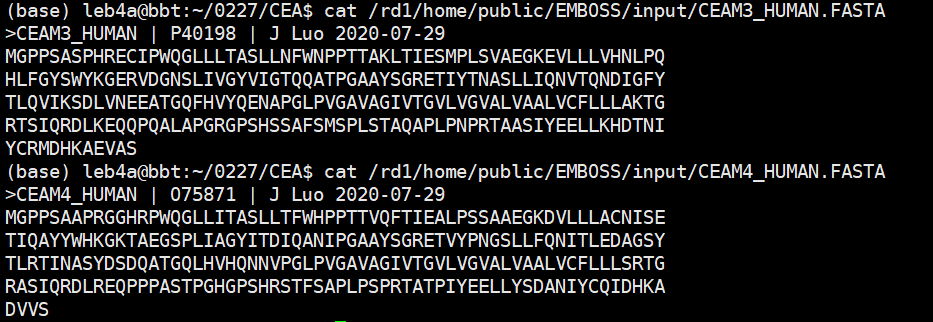
\includegraphics[width=0.8\textwidth]{./image/gdk/5.2.1.png}

输出结果:

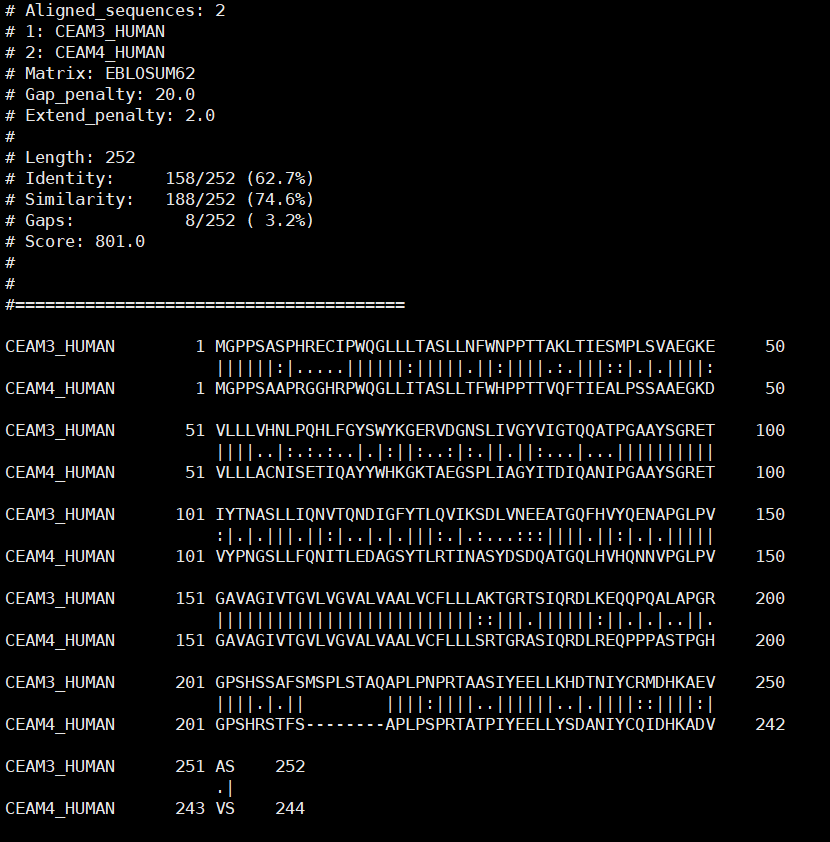
\includegraphics[width=0.8\textwidth]{./image/gdk/5.2.2.png}

\subsection{water}

water程序用于序列的局部比对。以人类CEAM3、、CEAM5蛋白质序列比对为例,使用water程序进行分析:

\begin{lstlisting}
    #! /bin/usr
    path="/rd1/home/public/EMBOSS/input"
    water ${path}/CEAM3_HUMAN.FASTA -sbegin 35 -send 142  \
	    ${path}/CEAM5_HUMAN.FASTA -sbegin 35 -send 142 \
	    ./CEAM3-CEAM5.WATER -gapo 20 -gape 2
\end{lstlisting}

\begin{quotation}
    -sbegin: 比对起始位点。

    -send: 比对终止位点。

    -gapo: 起始空位罚分,默认为10。

    -gape: 延伸空位罚分,默认为0.5。
\end{quotation}

CEAM3、CEAM5序列:

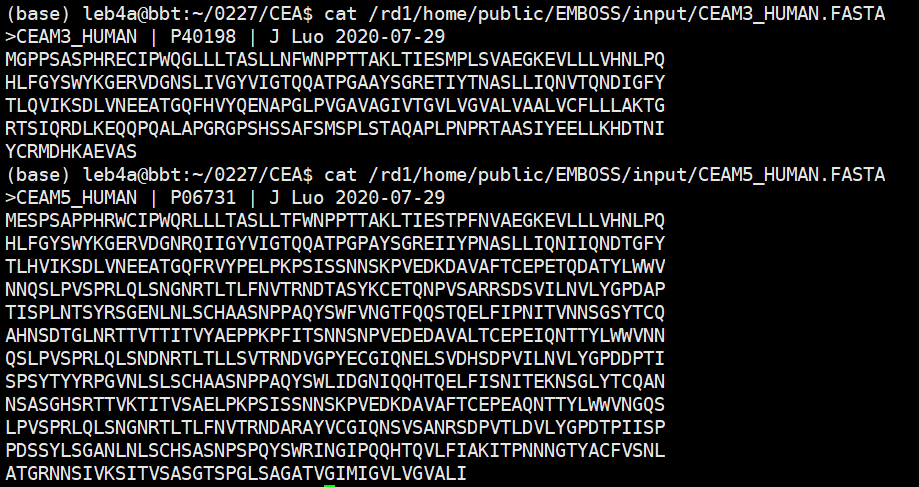
\includegraphics[width=0.8\textwidth]{./image/gdk/5.2.3.png}

输出结果:

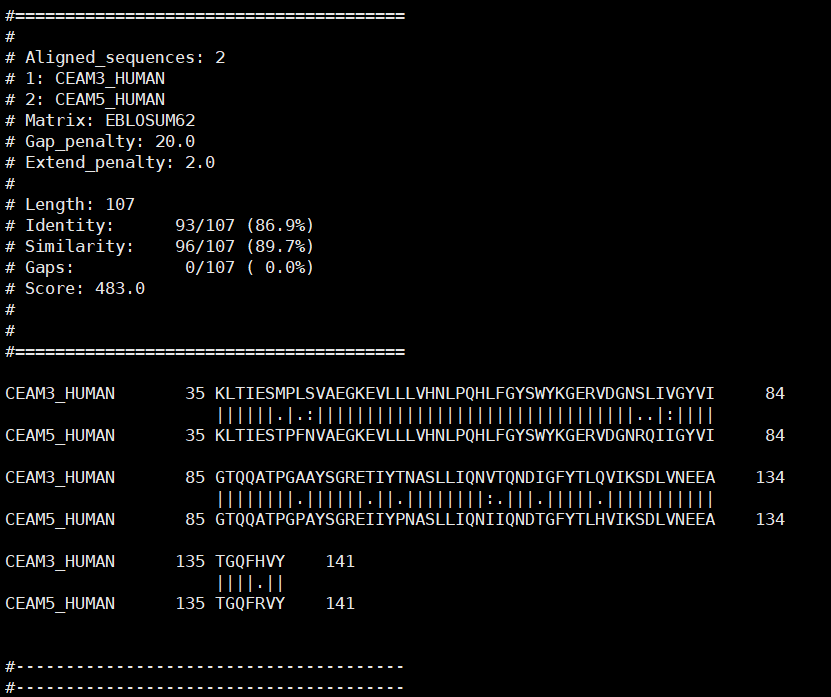
\includegraphics[width=0.8\textwidth]{./image/gdk/5.2.4.png}

\subsection{edialign}

edialign程序用于序列的多重比对。以人类所有CEA蛋白质序列比对为例,使用edialign程序进行分析:

\begin{lstlisting}
    #! /bin/usr
    path="/rd1/home/public/EMBOSS/input"
    edialign ${path}/12HUMAN_CEA.FASTA 12HUMAN_CEA.EDIA 12HUMAN_CEA.ALN
\end{lstlisting}

12个人类CEA氨基酸序列:

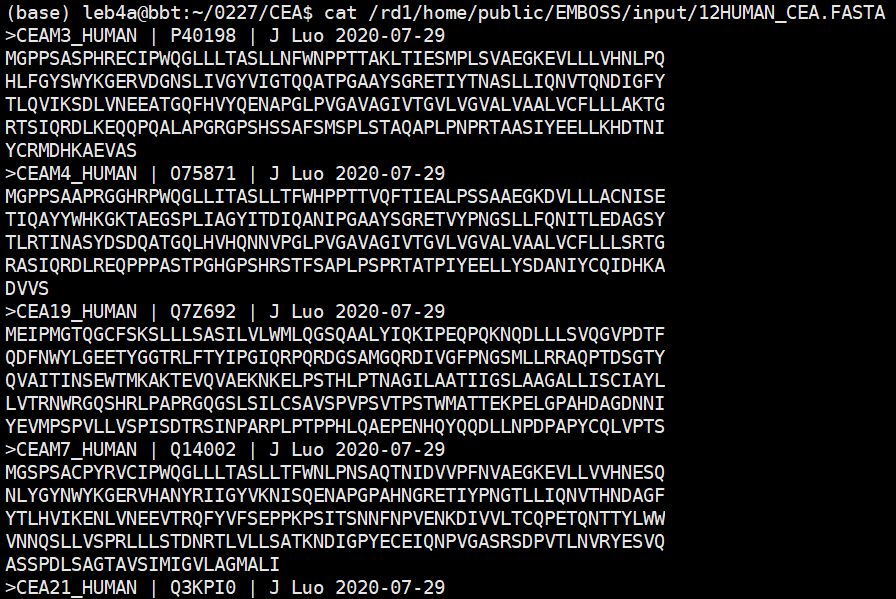
\includegraphics[width=0.8\textwidth]{./image/gdk/5.2.5.png}

部分输出结果:

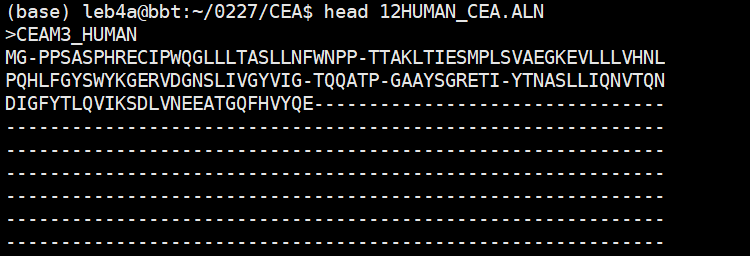
\includegraphics[width=0.8\textwidth]{./image/gdk/5.2.6.png}

\section*{参考资料}
[1]罗静初.EMBOSS和EMBnet[J].生物信息学,2021,19(04):223-231.

[2]罗静初.EMBOSS软件包序列分析程序应用实例[J].生物信息学,2021,19(01):1-25.                 % EMBOSS
\chapter{BLAST}

\section{背景}
对于研究序列同源性,序列的相似程度问题,序列比对算法是非常重要的工具。双序列比对可以采用基于动态规划算法的Needleman-Wunsch和Smith-Waterman算法,虽然精度高,但是计算消耗大,因此当与数据库进行比对时,这两种算法就显得力不从心。Blast采用启发式算法,通过丢失灵敏度来减少运行时间,以实现序列与大规模数据库的比对。


\section{BLAST}
BLAST(Basic Local Alignment Search Tool)算法的基本思想是通过产生数量更少的但质量更好的增强点来提高比对的速度。算法的原理主要分为以下五步:(1)过滤:首先过滤掉低复杂度区域,即含有大量重复的序列;(2)Seeding:将Query序列中每k个字组合成一个表,即将一个序列拆分成多个连续的‘seed words’(通常蛋白质k=3,核酸k=11);(3)比对:列出我们所关心的所有可能的字组,再配合置换矩阵给出高分值的字组并组织成快速搜索树结构或者哈希索引,因此此步骤可以快速搜索出大数据集中的所有匹配序列,找到每个seed words在参考序列中的位置;(4)延伸:当找到seed words的位置后,接下来需要将seed word延伸成长片段,延伸过程中,得分值也在变化,当得分值小于阈值时即停止延伸,最后得到的片段成为高分片段对,HSP(High-scoring segment pair);(5)显著性分析,最后我们使用如下公式计算E值,E值衡量了在随机情况下,数据库存在的比当前匹配分数更好的比对的数目,因此可以用该值作为指标评价HSP比对序列的可信度\par
$$ E = kmne^{-\lambda S}$$
其中,m是数据库长度,n是query的长度,S是HSP分数,其他两个参数是修正系数。
\subsection{BLAST的基本想法}
\begin{enumerate}
    \item 首先将输入序列切分成若干小段——seed words, 对于一个给定的字长 w (usually 3 for proteins and 11 for nucleotides), 将输入序列分成许多连续的 seed words
    \item 通过事先建立的索引表,在数据库中快速定位候选序列,以及在候选序列中的具体位置(通过正确设计索引结果,这一步可以在线性甚至常数时间范围内完成, 从而提高效率)
    \item 通过对所有的seed重复上述操作,就可以得到查询序列与候选序列之间的hit map ——最优比对对应的路径,应当平行于主对角线。
    \item 进一步去掉零散的hits,仅保留沿对角线方向上,有两个及以上连续hits的hit clusters, 以便进一步缩小搜索空间
    \item 以hit cluster为基础,向左右两个方向,延伸扩展,知道总分数的下降超过一个给定的x值之后,停止延伸
    \item 在扩展后的区域,应用动态规划算法,确定最终的比对
\end{enumerate}
\subsection{Word size和积分矩阵}
Word size和积分矩阵是BLAST算法中的两个重要参数。Word size(W)指的是在查询序列中用于匹配数据库序列的单词长度。积分矩阵(scoring matrix)用于计算序列比对的得分。
调整这些参数可以优化BLAST搜索。例如,如果T与W成比例缩放,则较小的word size会增加灵敏度并降低速度。W,T和积分矩阵之间的相互作用至关重要,明智地选择它们是控制BLAST速度和灵敏度最有效的方法

\section{BLAST比对工具}
BLASTP是蛋白序列到蛋白库中的一种查询。库中存在的每条已知序列将逐一地同每条所查序列作一对一的序列比对。\par
BLASTX是核酸序列到蛋白库中的一种查询。先将核酸序列翻译成蛋白序列(一条核酸序列会被翻译成可能的六条蛋白),再对每一条作一对一的蛋白序列比对。\par
BLASTN是核酸序列到核酸库中的一种查询。库中存在的每条已知序列都将同所查序列作一对一地核酸序列比对。\par
TBLASTN是蛋白序列到核酸库中的一种查询。与BLASTX相反,它是将库中的核酸序列翻译成蛋白序列,再同所查序列作蛋白与蛋白的比对。\par
TBLASTX是核酸序列到核酸库中的一种查询。此种查询将库中的核酸序列和所查的核酸序列都翻译成蛋白(每条核酸序列会产生6条可能的蛋白序列),这样每次比对会产生36种比对阵列。

\begin{figure}[ht]
    \centering
    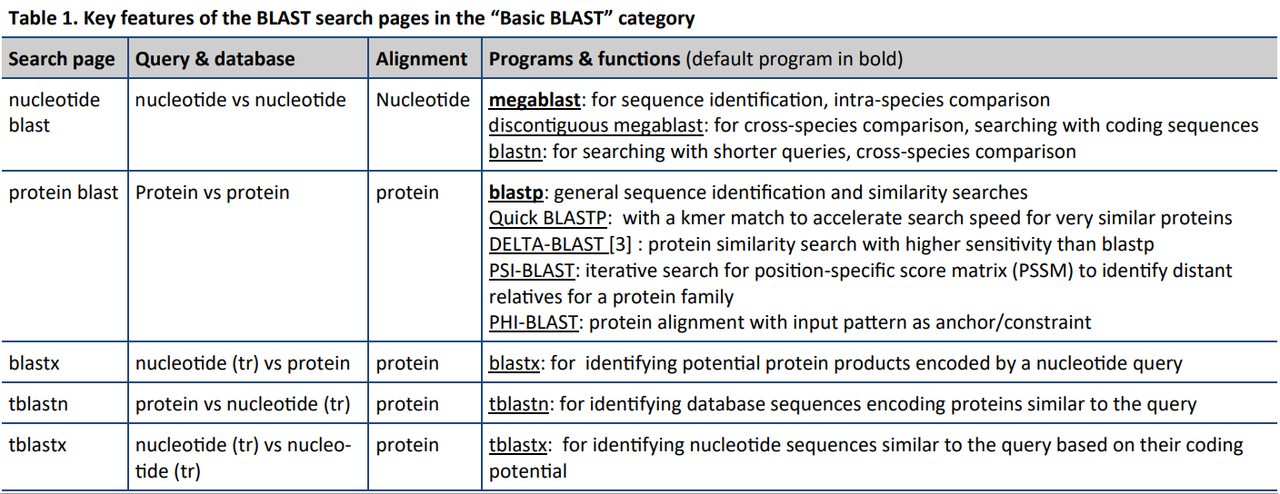
\includegraphics[width=10cm]{figure/blast.PNG}
\end{figure}

其中blastp中又有一些细分的方法,适用于比对不同相似程度的序列。quickblastp适用于快速比较非常相似的蛋白序列;delta-blast相比普通的blastp具有更高的灵敏度;PSI-blast使用PSSM打分矩阵,可以比较蛋白家族中关系较远的序列;PHI-blast将输入模式作为约束的蛋白比对,找到与查询序列具有一样的表达模式且具有同源性的蛋白序列。\par
其中blastn中也有一些细分的方法,具有不同的特点。除去标准方法blastn,magablast使用模糊搜索加快比对速度,用于优化非常相似的序列比较,或鉴定某段核酸序列是否在数据库中;DiscontiguousMagablast比blastn灵敏度更高,用于精确比对,适用于跨物种间的同源比对。\par
此外还有一些特殊功能的blast:
\begin{enumerate}
    \item Primer-BLAST: 使用primer3算法设计引物,并使用BLAST比对所选序列的模板特异性
    \item SmartBlast:可对使用者的蛋白查询进行处理,从数据库中选出5个最佳的蛋白匹配项,并给出一个简明的摘要
    \item lgBLAST:争对种系数据库搜索免疫球蛋白或T细胞受体序列以注释输入的免疫球蛋白序列,可以报告D/J区的相似对象;注释数据中的不同结构域
    \item MOLE-BLAST:从选定目标数据库中识别输入核苷酸序列的相邻序列(使用blast),然后使用多重序列比对(MUSCLE)根据序列相似性聚类。
    \item VecScreen:根据已知载体库和其他人工序列筛选输入的核酸序列,确定污染
    \item CD-search:与保守结构域数据库做比较,根据数据库检索蛋白序列进行功能分析
    \item CDART:识别输入蛋白序列中的保守结构域,然后寻找含有这些保守结构域额其他序列。
    \item Targeted loci:从细菌和古菌中的16S rRNA,或真菌的18S,28S和ITS中搜索仔细挑选的核苷酸序列,用于物种鉴定的需要
\end{enumerate}

\section{blast本地化安装配置}
配置local BLAST可以有效增加BLAST稳定性和比对速度。local BLAST由ncbi BLAST和数据库组成,用户可根据自己需要的数据库选择性下载,如rna\_reference数据库300GB左右,rna\_select数据库不超过50GB。

\subsection{准备工作}
源码安装BLAST
\begin{lstlisting}
# 复制安装包到目标目录
cp /rd1/home/public/BLAST/BLAST_TOOL/ncbi-blast-2.13.0+-x64-linux.tar.gz ~/install 

# 解压解包
gunzip ncbi-blast-2.13.0+-x64-linux.tar.gz
tar xvf ncbi-blast-2.13.0+-x64-linux.tar

# 复制可执行程序
cp -rf install/ncbi-blast-2.13.0+/bin/ ~/bin/blast_bin/

# 用户根目录隐藏文件.ncbirc用于指定数据库文件位置
# Specifies the path where BLAST databases are installed
[BLAST]
BLASTDB=/rd1/home/public/blast_db
# 自己下载的数据库或自己构建的数据库也需要添加到此配置文件中

# 环境配置
### BLAST环境变脸配置
### .bashrc文件
# add the following code to the ~/.profile using vim/nano or other editor
# "~/.app/BLAST/ncbi-blast-2.13.0+/bin" is customized dir of your program's bin 

# set blast bin to PATH TangMingchuan 20230320
if [ -d "$HOME/.app/BLAST/ncbi-blast-2.13.0+/bin" ]; then 
    PATH="$HOME/.app/BLAST/ncbi-blast-2.13.0+/bin:$PATH"
fi

### .profile文件
# if running bash
if [ -n "$BASH_VERSION" ]; then
    # include .bashrc if it exists
    if [ -f "$HOME/.bashrc" ]; then
    . "$HOME/.bashrc"
    fi
fi

# set PATH so it includes user's private bin if it exists
if [ -d "$HOME/.local/bin" ] ; then
    PATH="$HOME/.local/bin:$PATH"
fi

source ~/.bashrc
\end{lstlisting}

\subsection{进行本地blast}

数据库可以从NCBI上下载构建好的数据库,也可以自己构建数据库,这里选择自己构建数据库

\begin{lstlisting}
##### step0 下载NCBI数据库
# 查看可以下载的数据库
update_blastdb.pl --showall
# 如欲下载指定的数据库,如swissprot
update_blastdb.pl --decompress swissprot

##### step1 创建索引文件,建立索引所需数据库

ln -s /rd1/home/public/blast_data/sbp/ZMTF_PEP.FASTA . 
ln -s /rd1/home/public/blast_data/sbp/ZMTF_CDS.FASTA .
makeblastdb -dbtype prot -in ZMTF_PEP.FASTA -out ZMTF_PEP
makeblastdb -dbtype nucl -in ZMTF_CDS.FASTA -out ZMTF_CDS

### -in:待格式化的序列文件
### -dbtype:数据库类型,prot或nucl
### -out:个人数据库命名,之后使用数据库使用这个名称

##### step2 进行blast比对
## 根据不同的需求选择合适的blast工具
## 不同的blast工具的应用范围虽然不同,但是基本参数都是一致的,这里以blastp为例。


\end{lstlisting}

blastp的一般参数

\begin{enumerate}
    \item -query 指定查询序列
    \item -db 指定使用的数据库
    \item -out 指定输出文件名
    \item -evalue 指定可接受的最高假阳性期望
    \item -outfmt 指定输出文件的格式
    \item -word\_size 指定词长
    \item -matrix 指定计分矩阵
    \item -query\_loc 指定查询序列中要查询片段的起止位置
    \item -subject 指定使用的被查询的序列文件
    \item -subject\_loc 指定被查询序列文件的起始位置
    \item -max\_target\_seqs 指定搜素结果中显示的最大序列数目
\end{enumerate}

outfmt的类型共有18个
\begin{itemize}
    \item 0 = Pairwise,
    \item 1 = Query-anchored showing identities
    \item 2 = Query-anchored no identities
    \item 3 = Flat query-anchored showing identities
    \item 4 = Flat query-anchored no identities,
    \item 5 = BLAST XML,
    \item 6 = Tabular,
    \item 7 = Tabular with comment lines,
    \item 8 = Seqalign (Text ASN.1),
    \item 9 = Seqalign (Binary ASN.1),
    \item 10 = Comma-separated values,
    \item 11 = BLAST archive (ASN.1),
    \item 12 = Seqalign (JSON),
    \item 13 = Multiple-file BLAST JSON,
    \item 14 = Multiple-file BLAST XML2,
    \item 15 = Single-file BLAST JSON,
    \item 16 = Single-file BLAST XML2,
    \item 17 = Sequence Alignment/Map (SAM),
    \item 18 = Organism Report
    \item 其中6,7,10,17可以自定输出格式。
\end{itemize}

\begin{lstlisting}
blastq -query ZMTF_PEP.FASTA -db swissprot -out ZMTF_SW.txt -evalue 0.01 -outfmt 7 -word_size 3 -matrix PAM250
\end{lstlisting}                  % BLAST
\chapter{HMMER}

\section{HMMER简介}

\begin{quotation}
    HMMER is used for searching sequence databases for sequence homologs, and for making sequence alignments. It implements methods using probabilistic models called profile hidden Markov models (profile HMMs).

    HMMER is often used together with a profile database, such as Pfam or many of the databases that participate in Interpro. But HMMER can also work with query sequences, not just profiles, just like BLAST. For example, you can search a protein query sequence against a database with phmmer, or do an iterative search with jackhmmer.

    HMMER is designed to detect remote homologs as sensitively as possible, relying on the strength of its underlying probability models. In the past, this strength came at significant computational expense, but as of the new HMMER3 project, HMMER is now essentially as fast as BLAST.

    HMMER can be downloaded and installed as a command line tool on your own hardware, and now it is also more widely accessible to the scientific community via new search servers at the European Bioinformatics Institute.

    \textit{http://hmmer.org/}

\end{quotation}

\section{HMMER网站的四种搜索方法}

\subsection{phmmer}
\textit{single protein sequence against protein sequence database}

使用蛋白质序列在蛋白质数据库中搜索

phmmer is used to search one or more query protein sequences against a protein sequence database. For each query sequence in seqfile, use that sequence to search the target database of sequences in seqdb, and output ranked lists of the sequences with the most significant matches to the query.

\begin{quotation}

    \textit{https://www.mankier.com/1/phmmer}

\end{quotation}

\subsection{hmmscan}
\textit{single protein sequence against profile HMM library (Pfam,CATH-Gene3D,PIRSF Superfamily and TIGRFAMs).}

序列搜序列谱(以HMM构建的序列谱)

hmmscan is used to search protein sequences against collections  of protein profiles. For each sequence in seqfile, use that query sequence to search the target database of profiles in hmmdb, and output ranked lists of the profiles with the most significant matches to the sequence.

\begin{quotation}

    \textit{https://www.mankier.com/1/hmmscan}

\end{quotation}


\subsection{hmmsearch}
\textit{either multiple sequence alignment or profile HMM against protein sequence database.}

序列谱搜序列

hmmsearch is used to search one or more profiles against a sequence database. For each profile in hmmfile, use that query profile to search the target database of sequences in seqdb, and output ranked lists of the sequences with the most significant matches to the profile.

\begin{quotation}

    \textit{https://www.mankier.com/1/hmmsearch}

\end{quotation}

\subsection{jackhmmer}
\textit{iterative searches. lnitiated with a single sequence, a profileHMM or a multiple sequence alignment against a target sequence database.}

迭代搜索

jackhmmer iteratively searches each query sequence in seqfile against the target sequence(s) in seqdb. The first iteration is identical to a phmmer search. For the next iteration, a multiple alignment of the query together with all target sequences satisfying  inclusion thresholds is assembled, a profile is constructed from this alignment (identical to using hmmbuild on the alignment), and profile search of the seqdb is done (identical to an hmmsearch with the profile).

\begin{quotation}
    \textit{https://www.mankier.com/1/jackhmmer}
\end{quotation}

\section{Hmmer的网站使用实例:以jackhmmer为例}

WSL提供了一个完整的Linux内核,但它不是一个虚拟机。相反,WSL提供了一个Linux系统调用兼容层,以便可以在Windows上运行原生Linux二进制文件。这意味着您可以在Windows上运行Linux命令行工具、脚本和应用程序,而无需使用虚拟机或双引导设置。


(1)在uniprot上下载目标蛋白序列

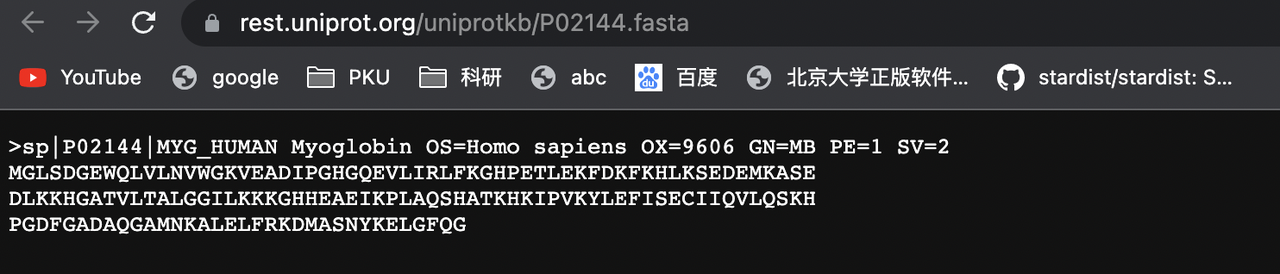
\includegraphics[width=0.8\textwidth]{./image/gdk/7.4.1.png}

(2)登陆hmmer网址-search-jackhmmer,输入序列

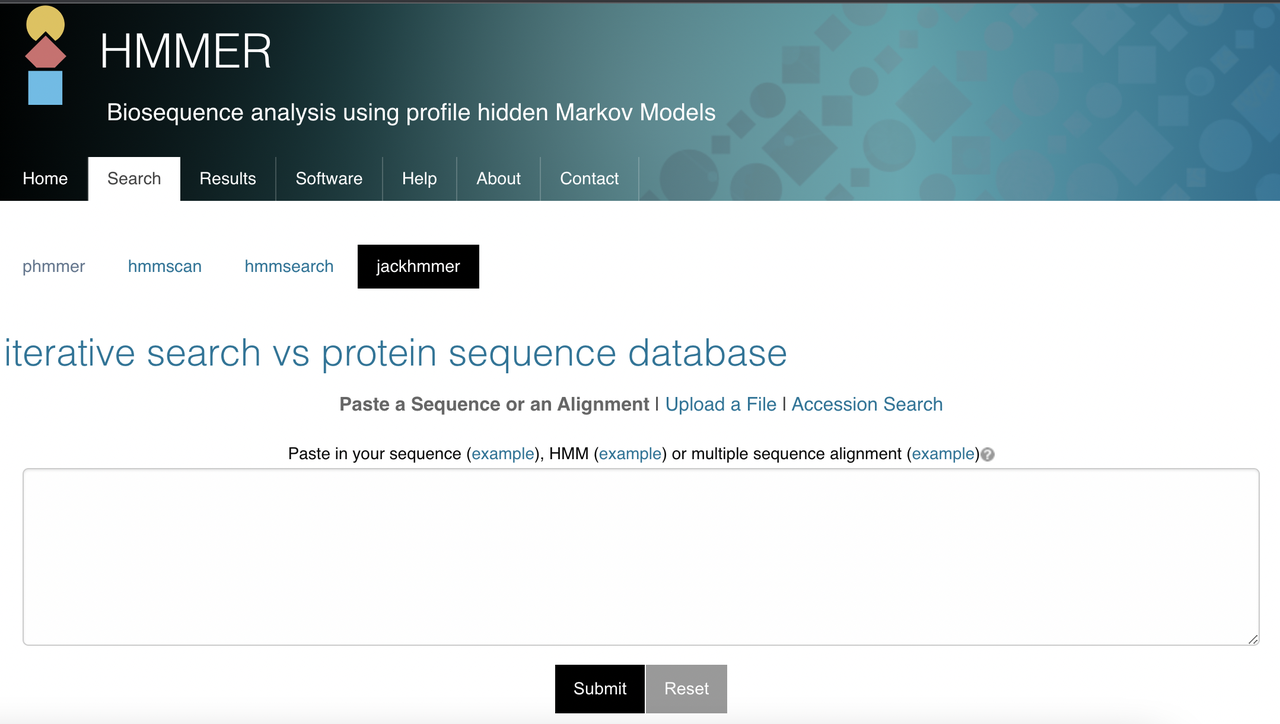
\includegraphics[width=0.8\textwidth]{./image/gdk/7.4.2.png}

(3)选择比对数据库与评估标准

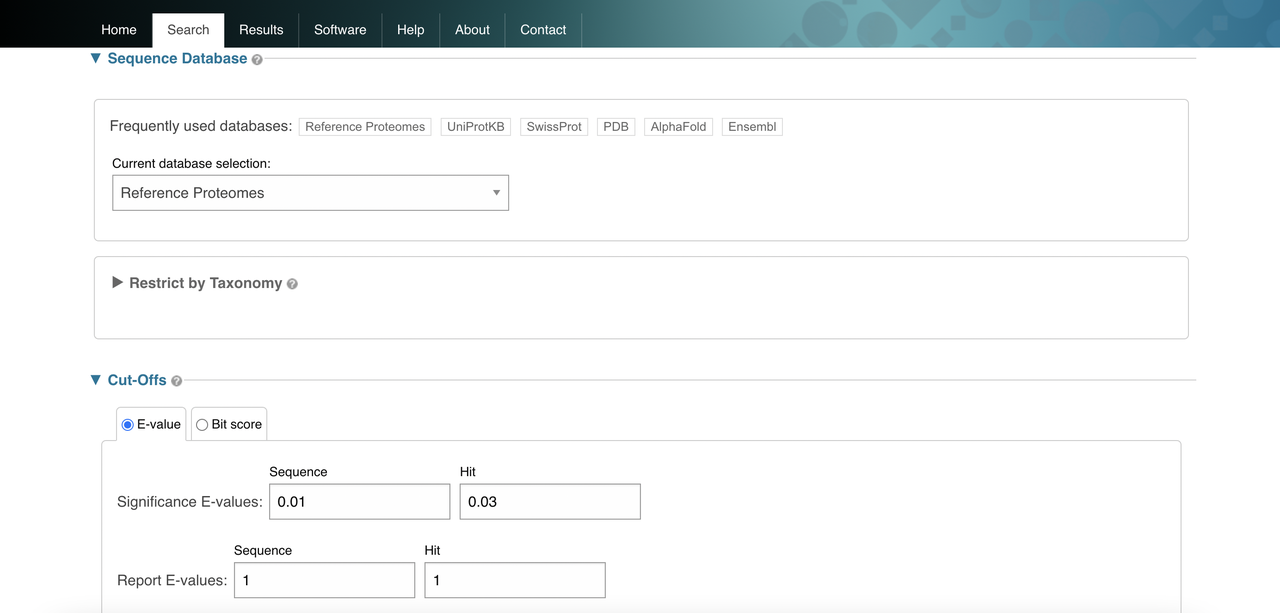
\includegraphics[width=0.8\textwidth]{./image/gdk/7.4.3.png}

(4)得到比对结果


\includegraphics[width=0.8\textwidth]{./image/gdk/7.4.4.png}

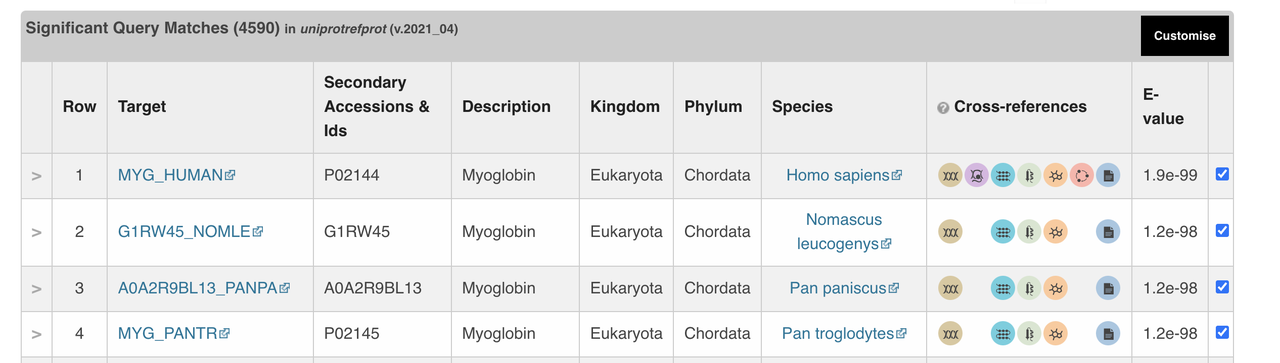
\includegraphics[width=0.8\textwidth]{./image/gdk/7.4.5.png}


(5)右上角customise可以选择需要列举的属性

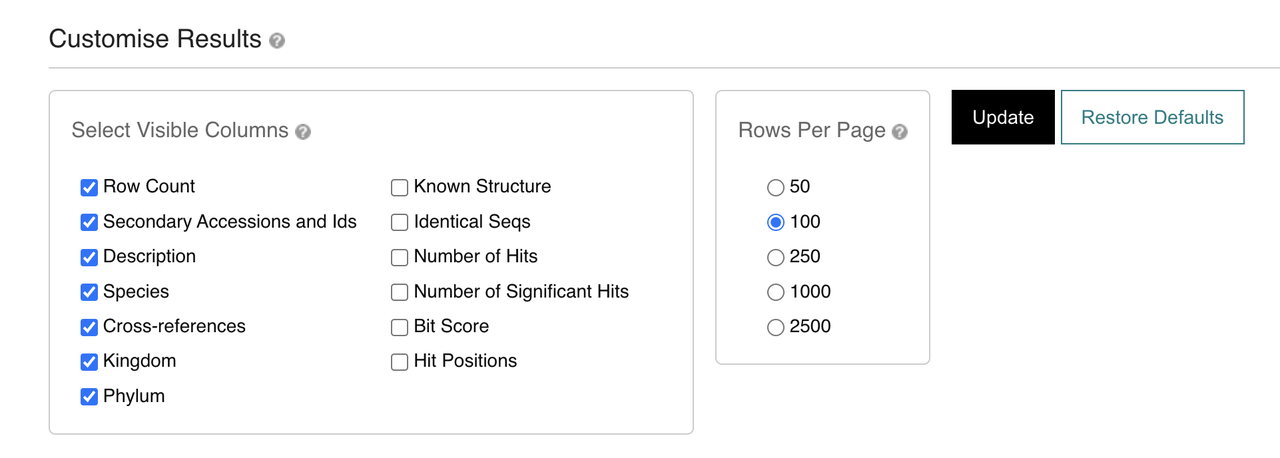
\includegraphics[width=0.8\textwidth]{./image/gdk/7.4.6.png}

(6)点击序列可以看到详细的对比情况

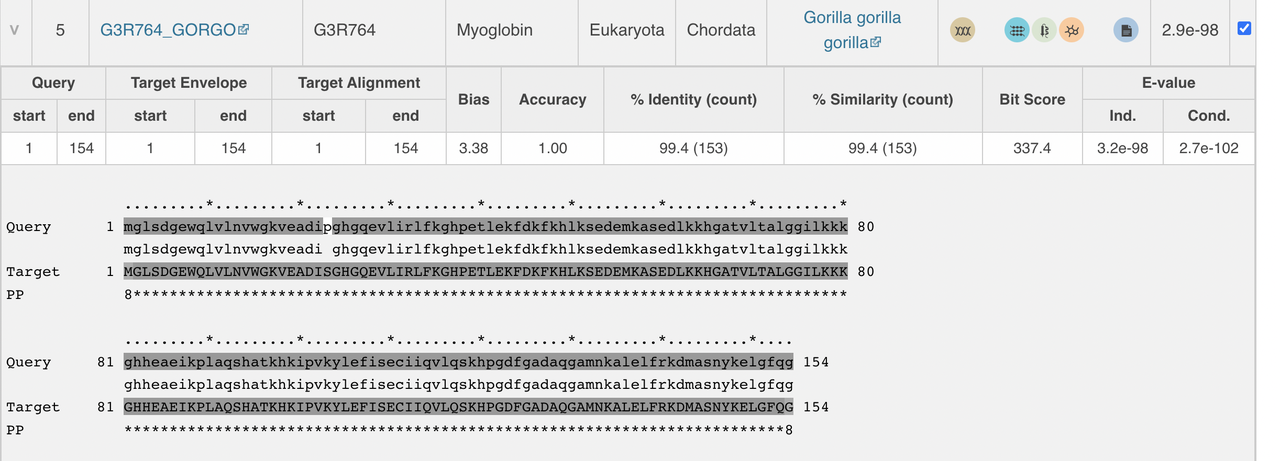
\includegraphics[width=0.8\textwidth]{./image/gdk/7.4.7.png}

(7)点击taxonomy可以得到分类图,其中的每一个节点都可以当作筛选的标准

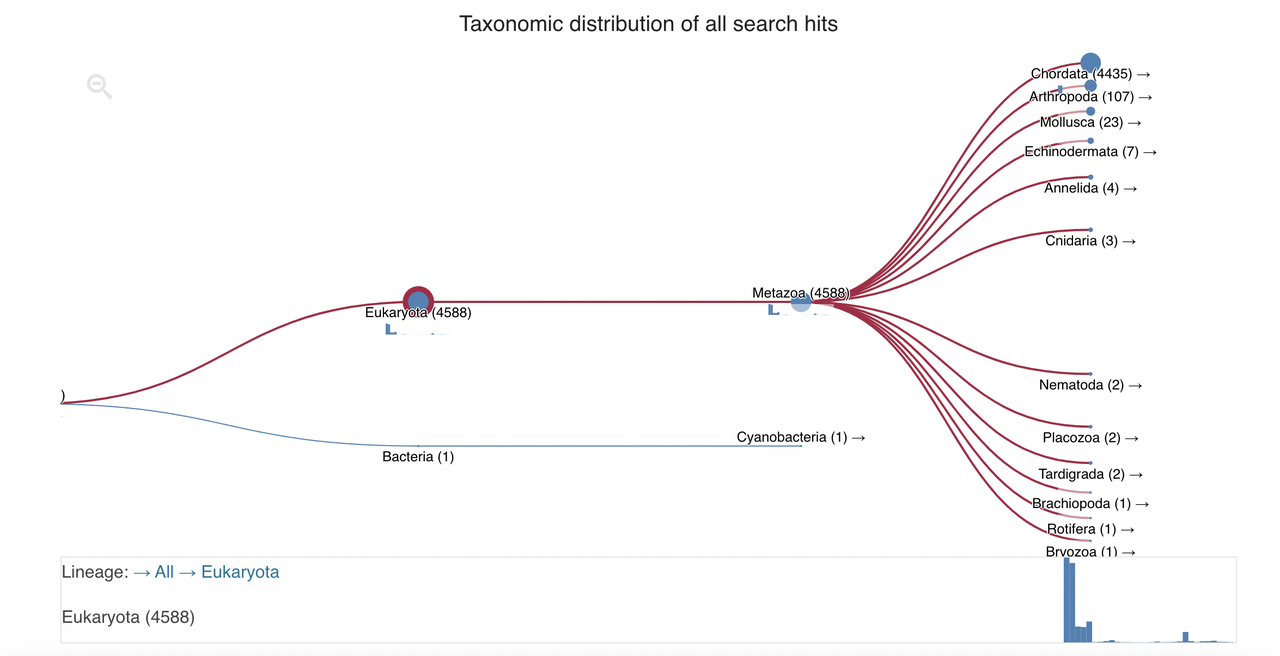
\includegraphics[width=0.8\textwidth]{./image/gdk/7.4.8.png}

(8)点击一轮迭代的右下角的“next iteration”,进行下一轮的迭代

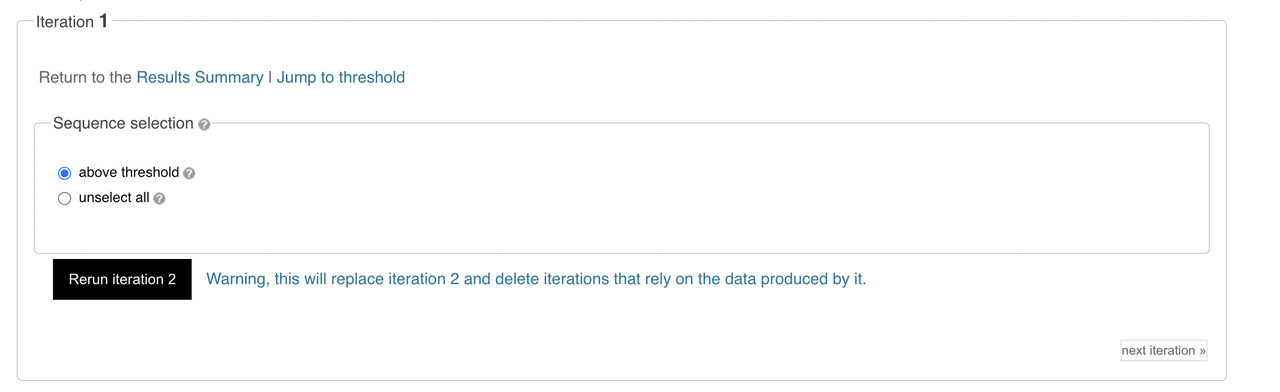
\includegraphics[width=0.8\textwidth]{./image/gdk/7.4.9.png}

(9)得到E-value极低的比对结果,此外还能得到Model Position图

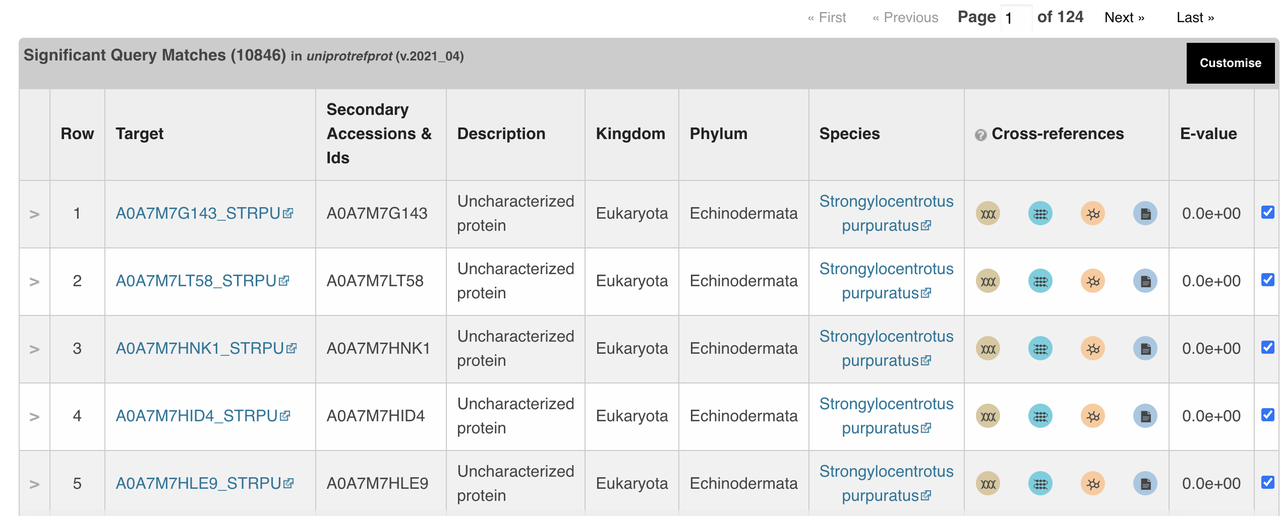
\includegraphics[width=0.8\textwidth]{./image/gdk/7.4.10.png}

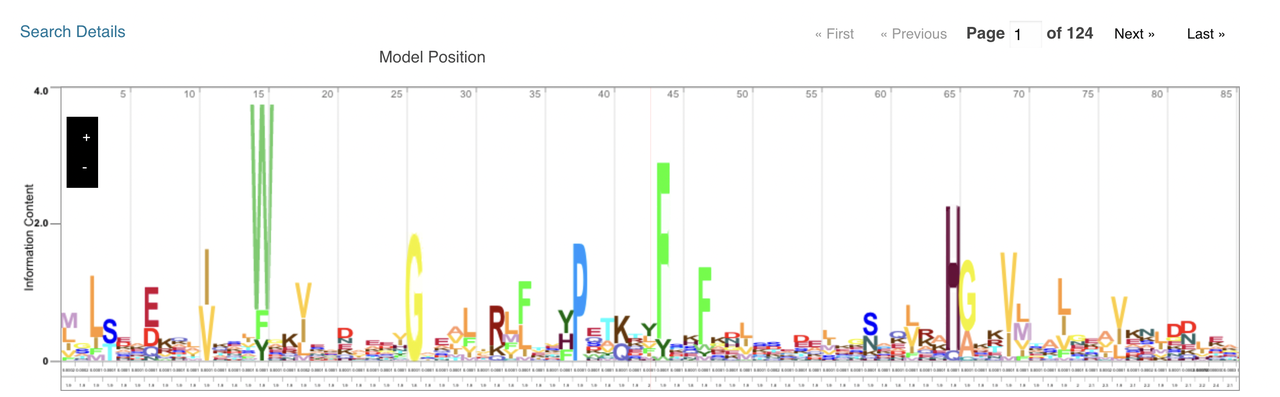
\includegraphics[width=0.8\textwidth]{./image/gdk/7.4.11.png}

\section{在python上使用HMMER}

将下列代码引入python中,并下载HMMER对应的数据库

\begin{lstlisting}
    import pyhmmer
    with pyhmmer.easel.SequenceFile("pyhmmer/tests/data/seqs/938293.PRJEB85.HG003687.faa",                                      digital=True) as seq_file:
        sequences = list(seq_file)
    with pyhmmer.plan7.HMMFile("pyhmmer/tests/data/hmms/txt/t2pks.hmm") as hmm_file:
        for hits in pyhmmer.hmmsearch(hmm_file, sequences, cpus=4):
            print(f"HMM {hits.query_name.decode()} found {len(hits)} hits in the target sequences")

\end{lstlisting}                  % HMMER

\chapter{TBtools}

\section{TBtools简介}

(a Toolkitfor Biologists integrating various biological data-handling tools),
是一款集成了blast、KEGG等模块的生信分析软件(软件包主页\textit{https://github.com/CJ-Chen/TBtools/releases}).

TBtools有共130余种不同功能,是一款强大的生信分析-可视化软件。

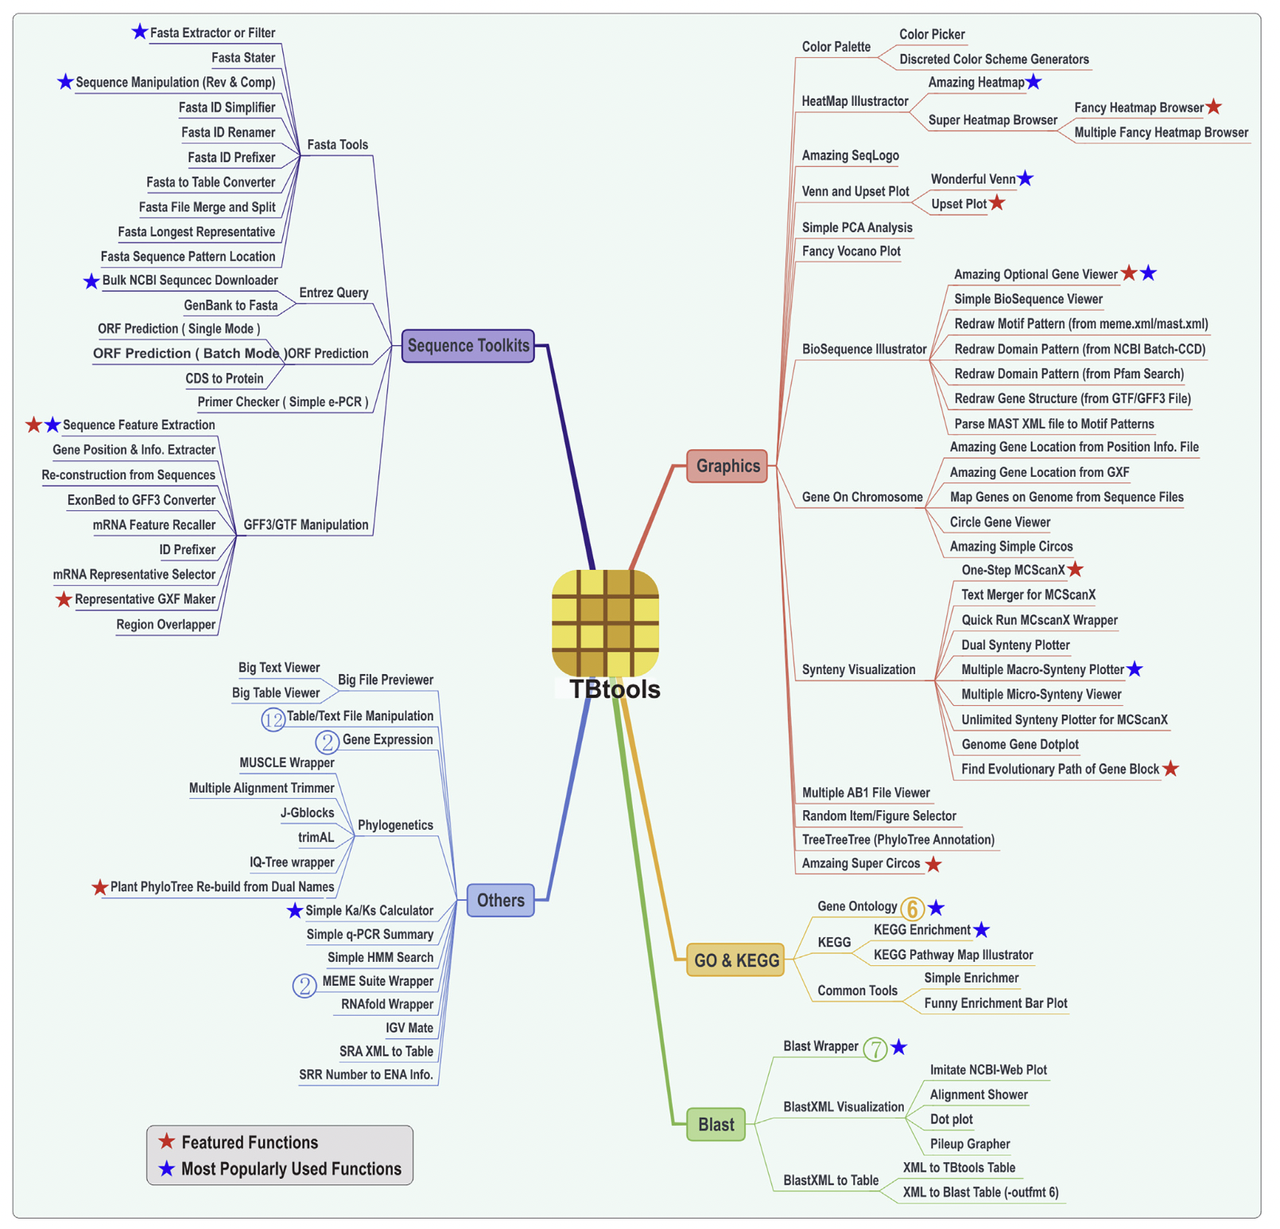
\includegraphics[width=0.8\textwidth]{./image/gdk/8.1.1.png}

\begin{quotation}
    功能总览,图源:https://www.yuque.com/cjchen/hirv8i
\end{quotation}

TBtools是为交互式数据表示而开发的,而数据可视化和表示是生物信息分析不可或缺的部分。与通常生成不可编辑图形的常规图形生成器不同,TBtools生成充满可编辑特征的交互图形。TBtools中集成了一个名为“JIGplot”(Java交互式图形)的新开发的绘图引擎,可以快速修改各种图形功能。

例如:可以在control panel上快速的调节绘画时的各种参数,修改生成的可视化图片,为用户提供了很大的方便性。

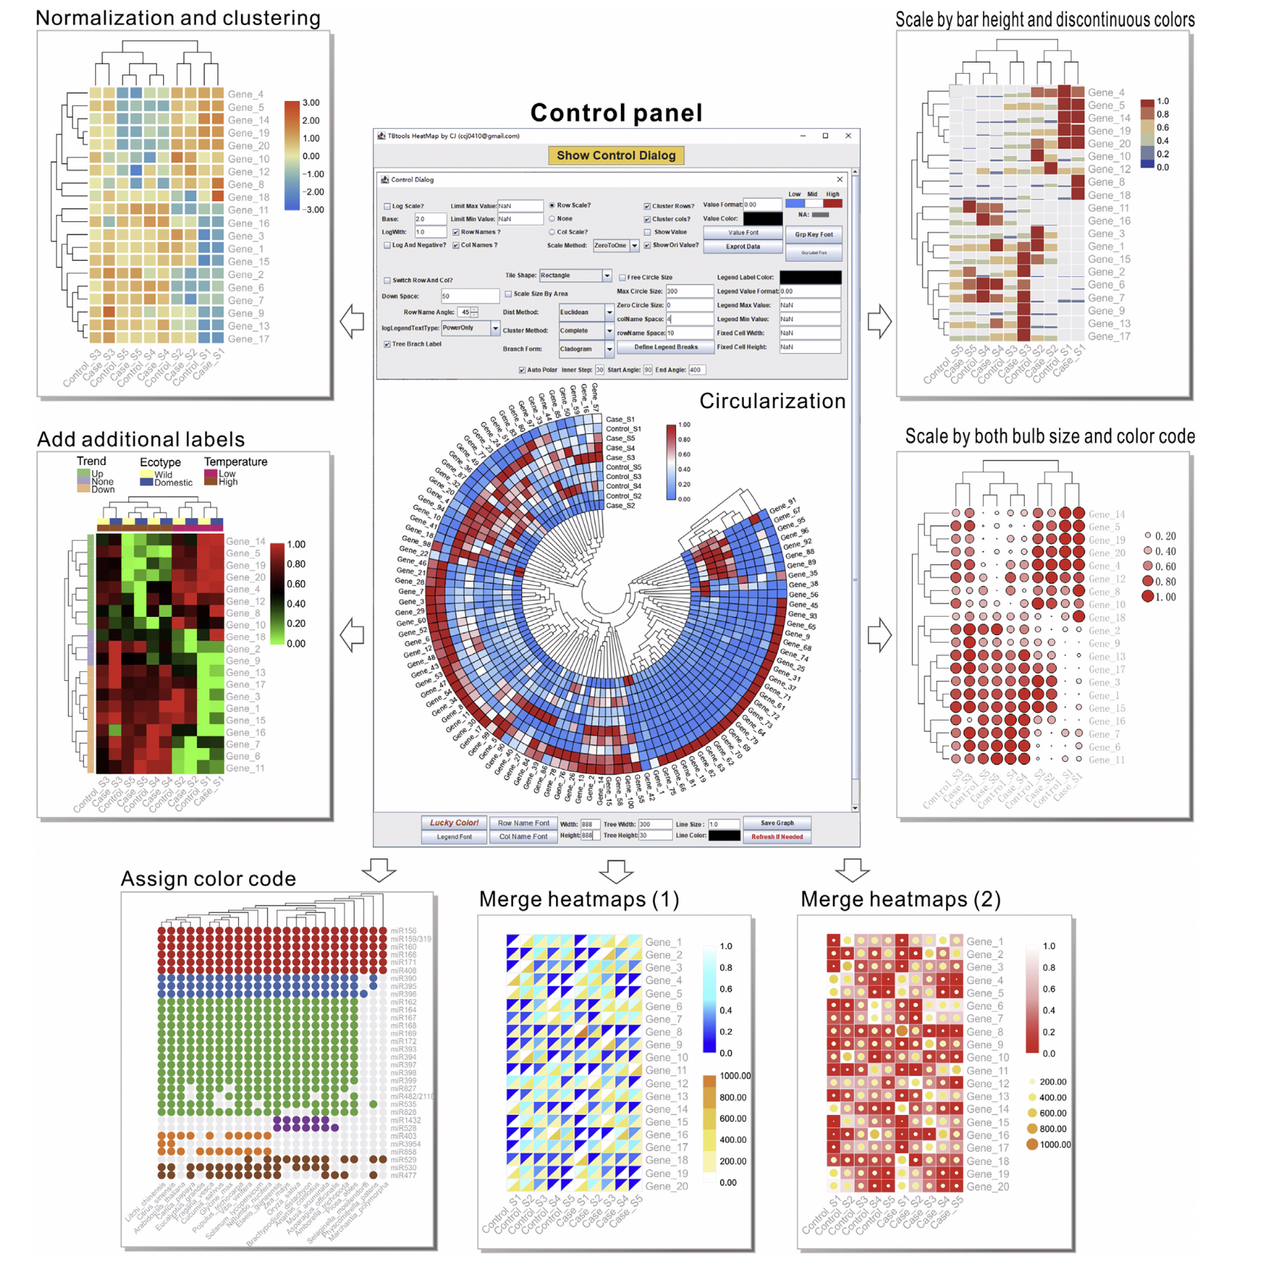
\includegraphics[width=0.8\textwidth]{./image/gdk/8.1.2.png}

本小节中,只对TBtools的功能进行简要介绍,不包含详细的案例分析。

\section{软件功能实例}

\subsection{ORF预测}
\subsubsection{背景}
预测ORF(Open Reading Frame)时,从mRNA角度(起始密码子,canonical或non-canonical等),蛋白质角度(蛋白产物稳定性、是否具有功能等)进行预测。
\subsubsection{常用的ORF预测软件——OrfM}
以往寻找终止密码子的方式:将原始序列切成6种不同的frame,逐个扫描获得终止密码子。

OrfM(\href{https://security.feishu.cn/link/safety?target=https%3A%2F%2Facademic.oup.com%2Fbioinformatics%2Farticle%2F32%2F17%2F2702%2F2450737&scene=ccm&logParams=%7B%22location%22%3A%22ccm_docs%22%7D&lang=zh-CN}{fast open reading frame predictor for metagenomic data})
直接在原始的核苷酸序列种寻找终止密码子,使用Aho-Corasick算法

Aho-Corasick:

    A. 根据已有的数据建立有限的目标pattern和模式匹配机
    B. 使用模式匹配机对文本字符串进行单遍处理。

构建模式匹配机所需的时间与pattern长度的总和成正比。

模式匹配机在处理文本字符串时进行状态转换的次数与关键字的数量无关。

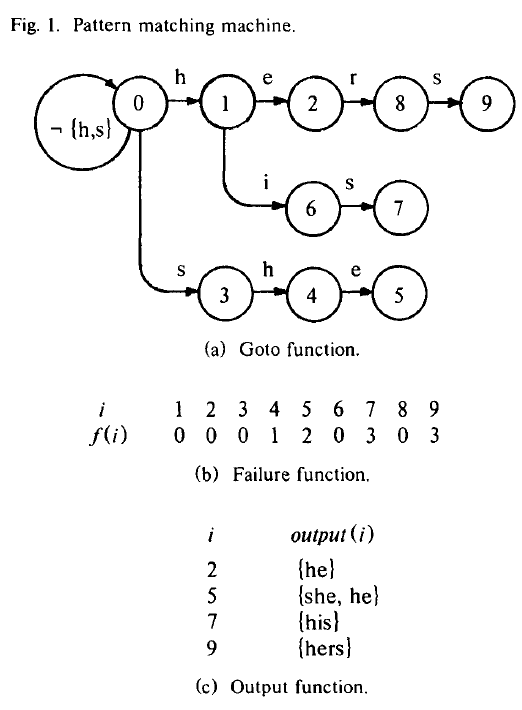
\includegraphics[width=0.6\textwidth]{./image/gdk/8.2.1.png}
\subsubsection{TBtools中的ORF prediction}
可进行单条序列中ORF的预测

批量序列中ORF的预测

批量CDS对蛋白质的转化(是否考虑密码子偏好性)



\subsection{基因富集分析}
\subsubsection{背景}
GO(gene ontology,基因本体论)的主要目的是归类,统一生物学方言(不同的生物学数据库可能会使用不同的术语)。

GO是一个有向无环图(DAG)本体,主要形式是term标记,每个GO term代表一种功能描述,都属于ontology。

GO总共分成三个ontology:molecular function(MF), cellular component(CC)和biological process(BP)。

不同GO term之间存在多种关系,常见的主要是is\_a和part\_of和两种关系.

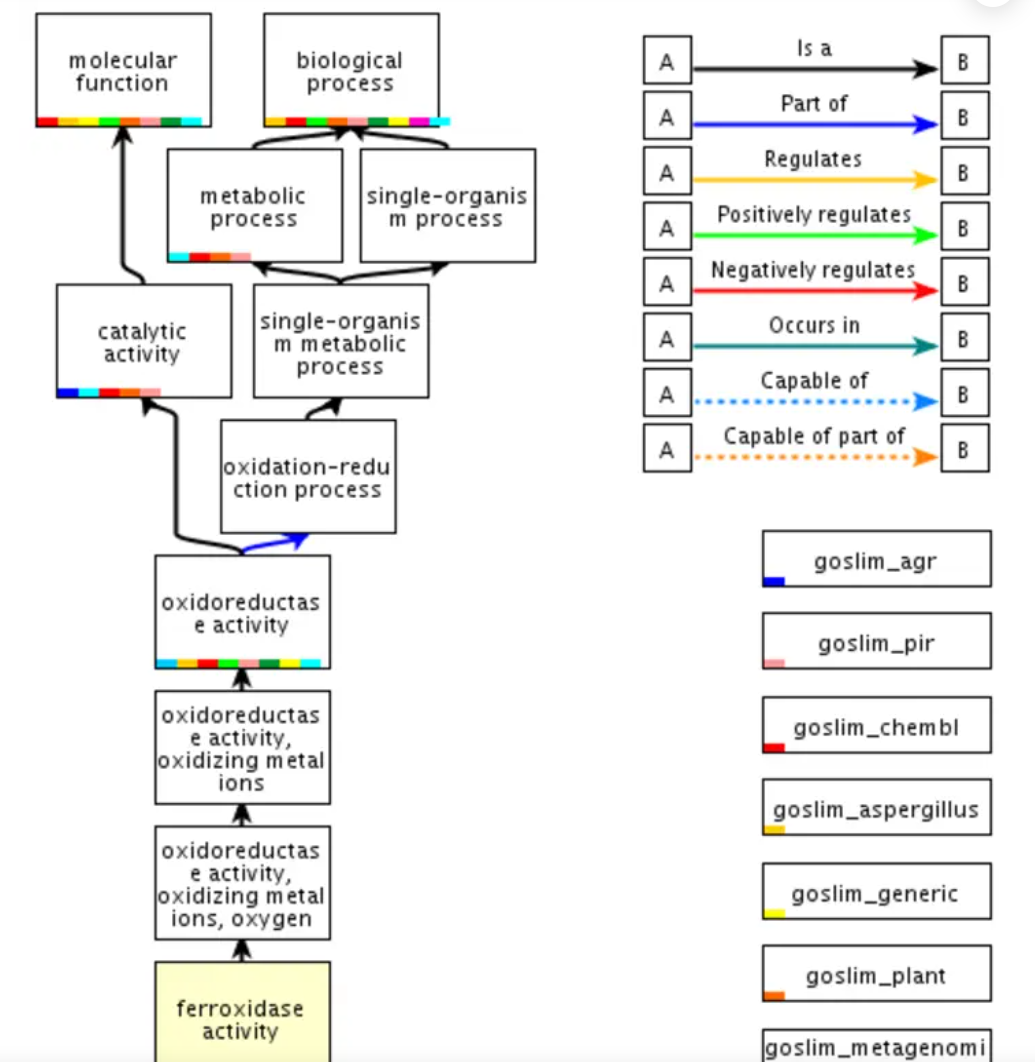
\includegraphics[width=0.75\textwidth]{./image/gdk/8.2.2.png}

\subsubsection{基本原理介绍}
如已有一基因集合(如差异表达基因集合或ChIP-seq的Peaks或GWAS定位的系列区间),
及有一个功能标签(例如如生长素信号转导相关 )。

假定某物种共有100个基因,其中20个基因与生长素信号转导相关,80个基因未注释到与生长素信号转导相关(在该注释库下被认为于无关)。
对植株进行处理,通过差异表达分析鉴定到10个差异表达基因,其中2个与生长素信号转导相关,而另外8个则没注释到生长素信号转导相关。

结果如下:


\includegraphics[width=0.8\textwidth]{./image/gdk/8.2.3.png}

检测结果中用于差异分析的基因集合中与生长素相应相关的基因比例与基因全集中与生长素相应相关的基因比例(背景比例相同),说明没有富集。

\begin{quotation}
    注意:

    1. 区别“富集”和“富集显著”:上述按理,若实验组基因集合中具有感兴趣标签的基因的比例超过背景比例,那么这种情况类比上,就是“富集”,因为偏离了背景。但是通过检验,如果偏离程度不大,则不能排除这是一种随机波动;而如果显著偏离了背景分布,就是“富集显著”。
    
    2. 富集分析时,很多新接触的,搞错的往往就是没搞清楚原理,背景(基因全集) 和 实验组基因集合(基因选择集合)(如差异表达基因集合)。一定要注意,做基因功能富集分析是,背景注释指的是这个物种所有基因的功能注释信息而不是选择集的基因功能注释。比如,做拟南芥的,大概有2w+个基因的功能注释,拿这个做背景;而不是拿差异表达的几百上千个基因的注释做背景。
\end{quotation}

\subsubsection{TBtools实现GO富集分析}

需要准备三个文件:

a. go-basic.obo 文件,可以从http://purl.obolibrary.org/obo/go/go-basic.obo下载

b. 一个物种所有基因的GO注释文件

c. 一个基因选择集合,如实验组基因集合,如差异基因集合,或GWAS筛选出来的基因集合等

具体实现过程:

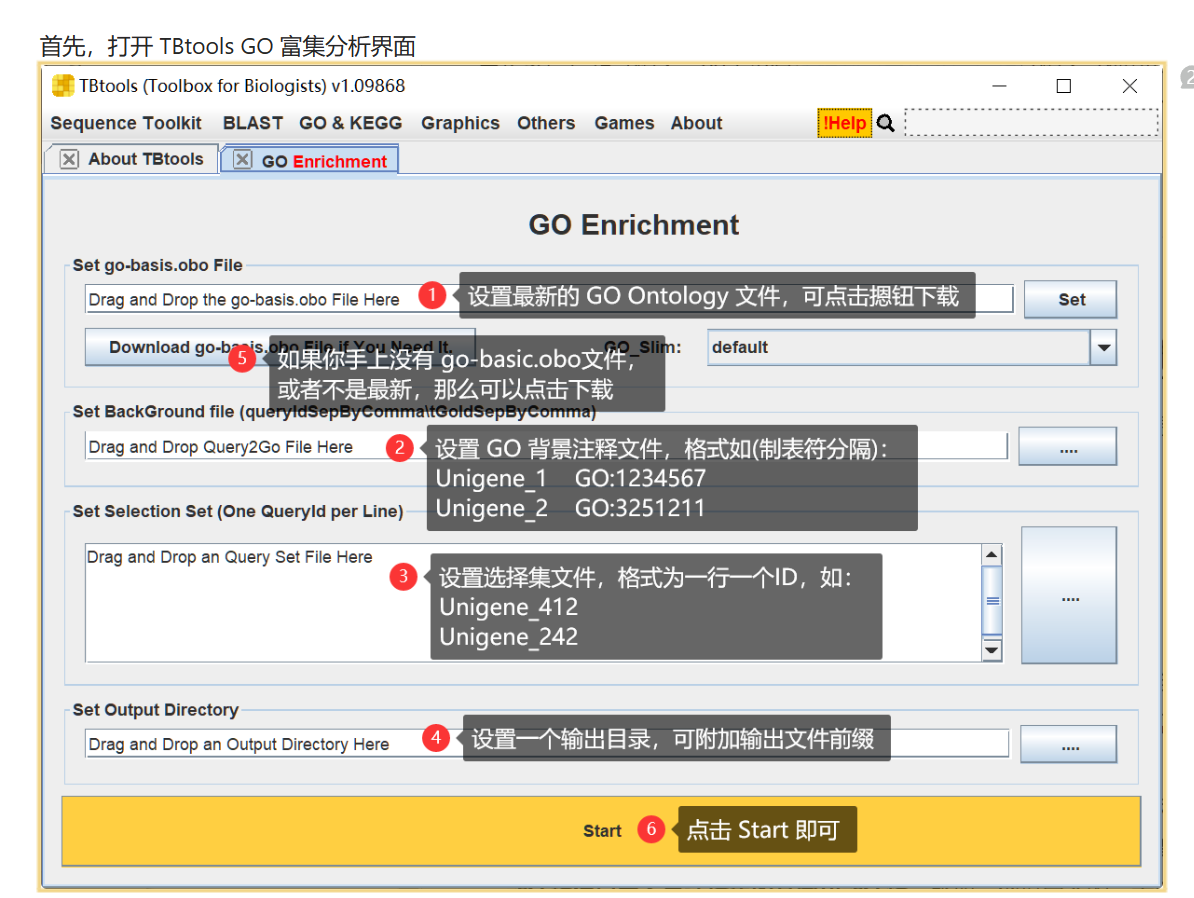
\includegraphics[width=0.8\textwidth]{./image/gdk/8.2.4.png}

\subsection{其他常见功能}

(1)eFP Browser 能够提供一个很简单便捷的方法用来可视化基因在宏观结构上的表达情况

(2)interactive heatmap:提供基因互作关系的程度关系

(3)simple circos:一种常见的基因比较分析可视化方法

......

\subsection{TBtools插件安装}

TBtools的插件模式允许用户在 TBtools 核心功能外按照自己需要安装特定插件,从而使用对应功能。这些插件可以直接在 TBtools 的 插件商店中找到。

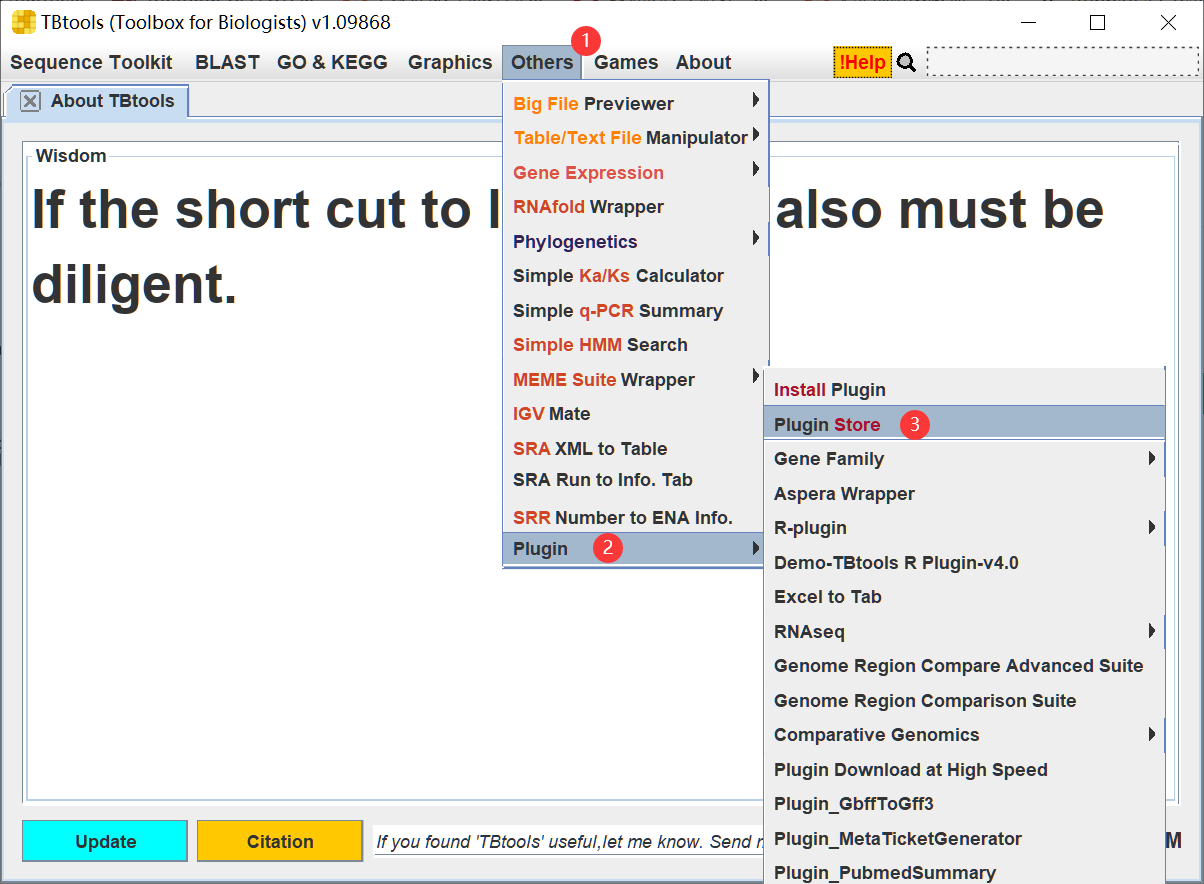
\includegraphics[width=0.8\textwidth]{./image/gdk/8.3.1.png}

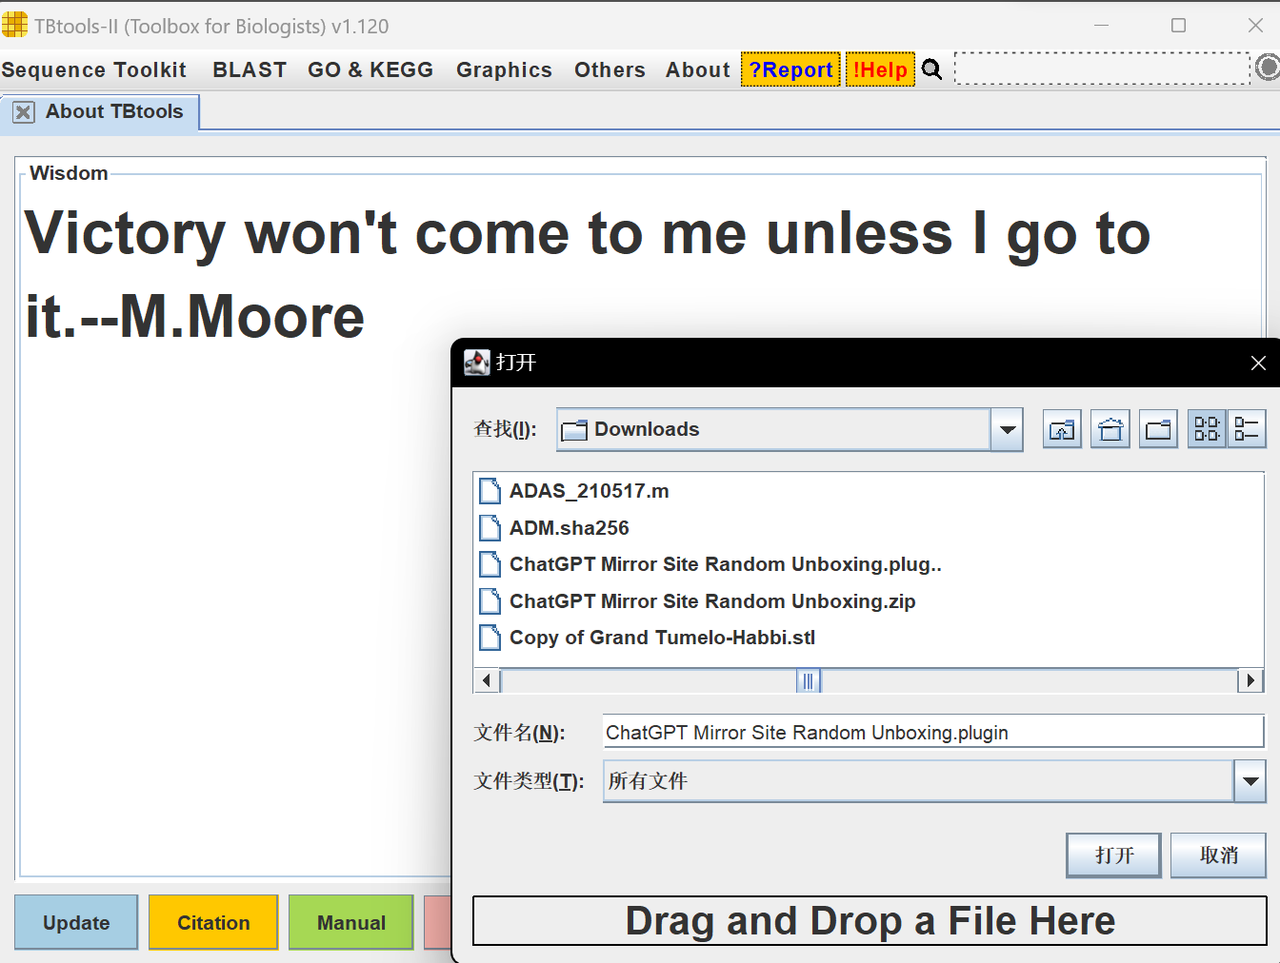
\includegraphics[width=0.8\textwidth]{./image/gdk/8.3.2.png}

安装完成后重启软件即可看见插件。

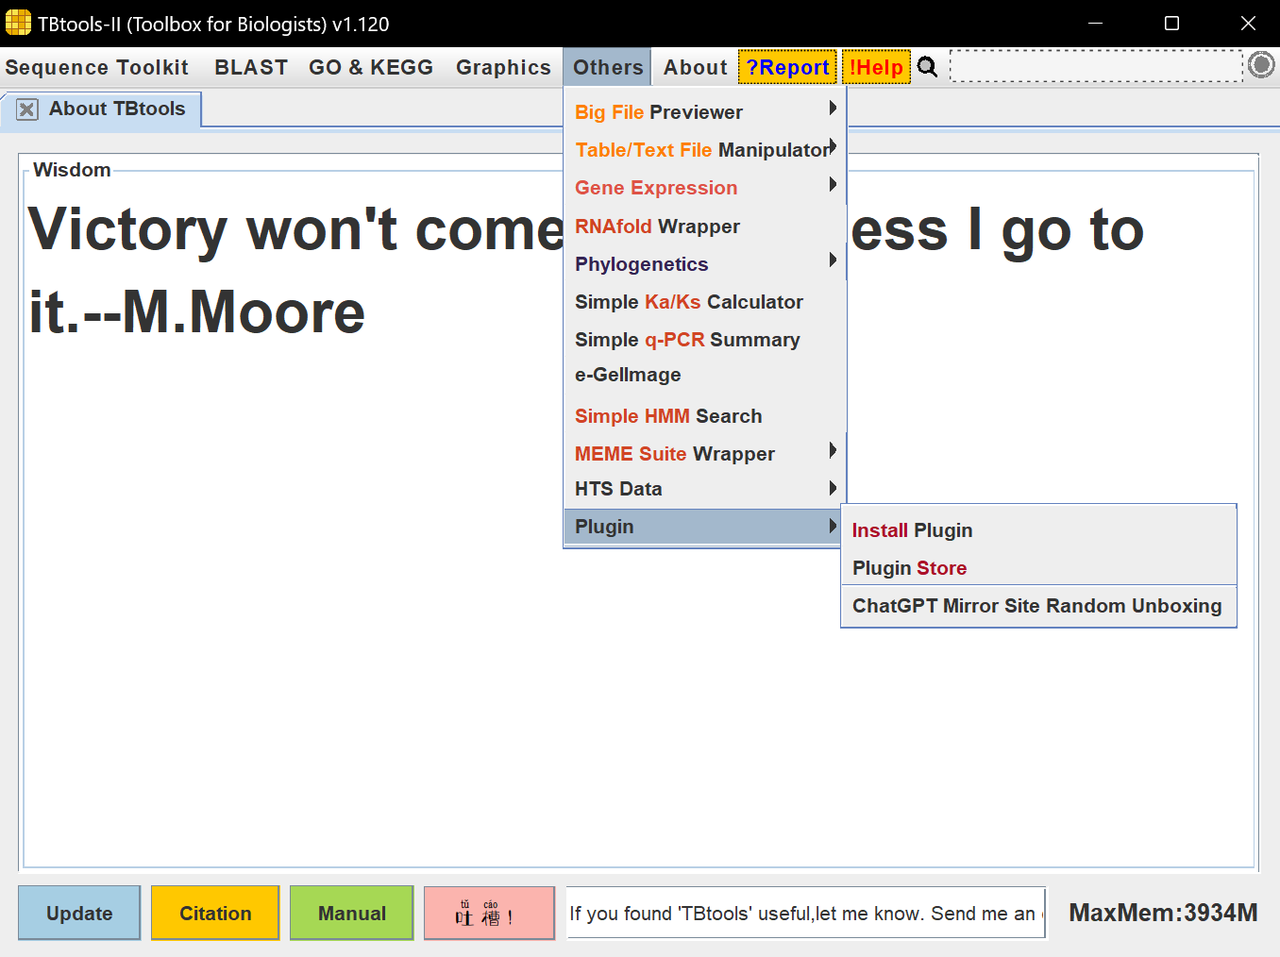
\includegraphics[width=0.8\textwidth]{./image/gdk/8.3.3.png}

\section*{参考资料}
\href{https://www.yuque.com/cjchen/hirv8i}{https://www.yuque.com/cjchen/hirv8i}

\href{https://zhuanlan.zhihu.com/p/144873860}{https://zhuanlan.zhihu.com/p/144873860}

\href{https://www.youtube.com/watch?v=O7\_w001f58c}{https://www.youtube.com/watch?v=O7\_w001f58c}                % TBtools

\chapter{ChIP-Seq项目实操}

本章将介绍ChIP-Seq的基本分析流程,包括上游分析和下游分析。\par
其中上游分析流程主要包括:
\begin{enumerate}
    \item fastq文件的质控、过滤、比对
    \item 比对文件的排序、过滤、去重、索引
    \item 查看ChIP-Seq分析的质量
\end{enumerate}

下游分析主要包括:
\begin{enumerate}
    \item call motif分析
    \item 与TSS的共定位分析
\end{enumerate}

本章涉及的软件较多,不能一一介绍其算法原理和详细的使用方法,因此对该项目代码中具体参数的调整需要争对不同的项目自行斟酌。但该项目代码依然具备较高的参考价值,可作为某些生信分析项目的通用分析模板。
感谢饶希晨师兄提供的大部分代码,我们在此基础上完成了后续代码的修改,并成功运行。\par
感谢李帅师兄的总结报告,为了该总结的完整性,我们在本章部分引用了李帅师兄的总结报告中的部分内容,如果对湿实验部分感兴趣,还请参考李帅的《生物信息技术期末总结》。


\section{背景介绍}

在此简要介绍该ChIP-Seq项目中使用到的一些基础概念。

\subsection{ChIP-Seq原理}

\textbf{染色质免疫共沉淀}(Chromatin Immunoprecipitation)实验主要用于目标蛋白会与基因组DNA中那些序列结合。其实验原理为,利用甲醛交联固定后,打断染色质DNA,与目标蛋白结合的DNA会与目标蛋白一起被目标蛋白的抗体免疫沉淀。\textbf{染色质免疫共沉淀测序技术}(ChIP-Seq)则是将上述免疫沉淀出的DNA接上测序接头,进行二代测序。
在此不再赘述湿实验的具体流程,本章主要聚焦该实验所得数据的生物信息学分析。ChIP-Seq的基本分析流程也可拓展应用到其他任何与\textbf{寻找目标核酸序列在基因组中的位置}相关的生信分析中。

\subsection{CTCF简介}
本章节使用的测序数据为CTCF蛋白的ChIP-Seq数据。\par
CCCTC-结合因子(CCCTC-binding factor, CTCF)是一种高度保守的锌指蛋白,可以作为转录激活因子、转录阻遏因子,此外还可以作为绝缘因子阻断增强子和启动子之间的通讯。\par
CTCF可以与染色质结构域边界结合的同时招募其他转录因子,并帮助真核基因组构建三维结构。\par
CTCF通过其11个锌指(ZF)定向结合众多CTCF结合位点(CBS)内的四个模块的特定序列元件,确定适当的全基因组染色质环相互作用。目前CTCF与CBS复合物的晶体结构已被解出。

\subsection{ChIP-Seq分析前的准备工作}
本项目的上游分析流程是许多生信分析共有的一般分析流程,包括质量控制、去接头、比对;比对文件的排序、转换、过滤、去重、索引。随后进行ChIP-Seq特有的分析,包括ChIP-Seq质量控制、富集峰的寻找。最后根据研究项目的目的可进行进一步下游分析,本项目进行了初步的下游分析,包括富集峰与转录起始位点(TSS)的共定位、峰基序分析(call motif)
\subsubsection{环境配置}

\begin{lstlisting}
    conda create -n chip-seq
    conda activate chip-Seq
    conda install fastqc 
    conda install cutadapt 
    conda install bowtie2 
    conda install samtools ## 操作比对结果文件的软件
    conda install macs2 ## 用于寻峰的软件
    conda install -c bioconda deeptools
    conda install -c idr ## 用于多样本合并的软件


    # meme套件和homer软件需要perl环境,建议编译安装perl环境后再编译安装上述软件
    # 下载meme套件安装包
    wget https://meme-suite.org/meme/meme-software/5.4.1/meme-5.4.1.tar.gz
    tar zxf meme-5.4.1.tar.gz
    cd meme-5.4.1
    ./configure --prefix=$HOME/meme --enable-build-libxml2 --enable-build-libxslt \par
    make
    make test
    make install

    wget http://homer.ucsd.edu/homer/configureHomer.pl
    perl configureHomer.pl -install
    Homer\_HOME=/Users/zhaohuanan/rxc/homer
    echo PATH="${Homer\_HOME}/bin:$PATH"
    chmod +x configureHomer.pl
    ./configureHomer.pl -install hg38


    # piacrd需要Java环境,建议安装openjdk
    sudo apt update 
    sudo apt install openjdk-17-jdk
    # 下载picard包,并添加至环境变量,http://broadinstitute.github.io/picard/
    java -jar /path/to/picard.jar -h 
    java -jar $PICARD -h 
    http://broadinstitute.github.io/picard/
\end{lstlisting}

\subsubsection{测序数据和参考文件的下载}
本项目使用的公共数据来自数据库ENCODE(DNA元件百科全书, Encyclopedia of DNA Elements) \par
项目数据的登录号为ENCSR617IFZ。实验数据总共有四个文件,分别是两个生物学重复的Read1和Read2,测序类型为双端101nt,文件格式为fastq。\par
其中生物学重复1测序数据注册号为ENCFF631JSV, ENCFF715KYL;生物学重复2的数据注册号为ENCFF002OWA, ENCFF833BQT。\par

\begin{figure}[ht]
    \centering
    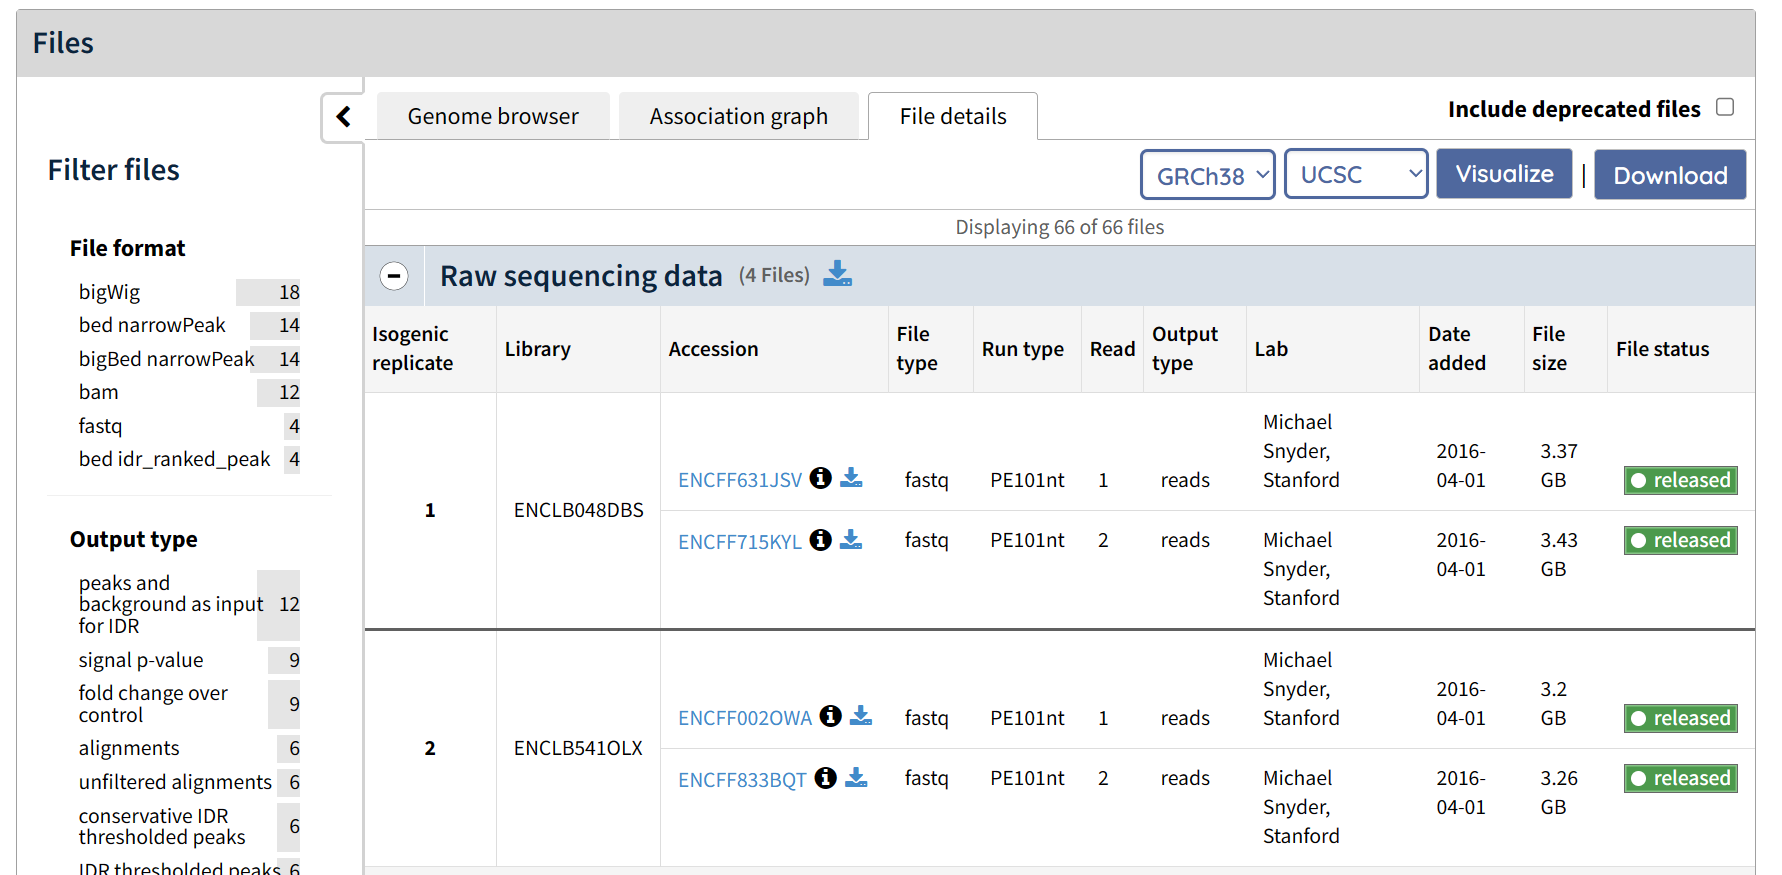
\includegraphics[width=10cm]{figure/encode_download.png}
\end{figure}
此外,在ChIP-Seq数据中寻找富集峰需要一份\textbf{未富集文库测序数据}作为参考(Input),本项目选用的数据注册号为:ENCFF873ZZU, ENCFF611URR.

\section{上游分析流程}
ChIP-Seq的一般分析流程
ChIP-Seq测序数据需要完成基本的NGS分析流程。该项目中,实验数据有两个生物学重复;此外为了call peak,另外需要一个未进行富集操作的测序数据作为参考。此三份数据采取完全相同的一般分析流程。\par
以本分析项目为例,作者希望建立一套尽可能自动化,规范化的流程。


\subsection{准备工作}
在分析开始之前,设置好自己的储存分配逻辑
\begin{lstlisting}
    #!/bin/bash

    ########
    # code for chipseq
    ########

    ##### 当前工作路径为 ##########
    ### 建议新建项目文件夹(此处为practice),并将该该文件夹设置为项目的工作路径
    # mkdir practice
    # cd practice
    # pwd
    # /home/wuhangrui/practice/

    ##### step0 创建原始数据与参考文件的软连接 #########
    ### 建议使用专门的存储空间或存储服务器存储原始数据和参考文件,并建议将其软链接到自己的工作路径下
    ## 在该项目的例子中,本章作者将下载的rawdata存放于nas中/nas\_data/whr/practice/chipseq/rawdata,
    ## 由于存储空间问题,本章作者在NAS中创建了存储中间结果的文件夹,并将该文件夹也软连接到工作目录下,以将中间结果文件也保存在NAS中
    ln -s /nas\_data/whr/practice/chipseq/ /home/wuhangrui/practice/chipseq
    cd ./chipseq

    # 创建存储中间结果的文件夹 
    mkdir 01\_fastqc 02\_cutadapt 03\_mapping 05\_peak\_calling

    # 读取样本名字
    cd ./rawdata

    # 把样本名字信息存放在config文件
    ls *\_r1.fastq.gz >config

    # 去掉后缀,仅保留名字信息
    sed -i "s/\_r1.fastq.gz//g" config

    cd /home/wuhangrui/practice/chipseq
\end{lstlisting}

\subsection{质量控制}
\begin{lstlisting}
    ##### step1 fastqc 质量控制 ##########
    ## 从nas里直接读取数据进行fastq,速度有点慢,建议在同一局域网下进行

    # 指示开始运行该软件的时间
    echo "fastq started at $(date)"

    # 对所有实验样本以及对照样本进行质控
    cat rawdata/config | while read id
    do
    fastqc -t 10 -o 01\_fastqc/ rawdata/${id}\_r1.fastq.gz rawdata/${id}\_r2.fastq.gz > 01\_fastqc/fastqc.log 2>&1
    done

    # 指示结束运行该软件的时间
    echo "fastq finished at $(date)"

    ### 软件参数说明
    ### fastqc [options] fastaq1 [fastq2 ...] 
    ### -t 指定使用的线程数
    ### -o 指定输出文件夹
\end{lstlisting}

\subsection{数据清晰和筛选}
\begin{lstlisting}
    ##### step2 cutadapt 数据清洗和筛选 ##########
    # 指示去除接头操作的开始时间
    echo "cutadapt started at $(date)"

    # 对所有实验组样本和对照组进行去接头和除去低质量读段的操作
    cat rawdata/config | while read id
    do
    cutadapt -j 10 \
    --time 1 -e 0.1 -O 3 --quality-cutoff 25 -m 55 \
    -a AGATCGGAAGAGCACACGTCTGAACTCCAGTCA -A AGATCGGAAGAGCGTCGTGTAGGGAAAGAGTGT \
    -o 02\_cutadapt/fixed\_${id}\_read1.fastq.gz -p 02\_cutadapt/fixed\_${id}\_read2.fastq.gz rawdata/${id}\_r1.fastq.gz rawdata/${id}\_r2.fastq.gz > 02\_cutadapt/cutadapt.log 2>&1
    done

    # 指示去接头操作的结束时间
    echo "cutadapt finished at $(date)"

    ### 程序参数说明
    ### -j 2 #设置线程数
    ### --times 1 # 只去处一次接头,因为接头只出现一次
    ### -e 0.1  # 去除的序列与adaptor相比,missmatch率低于该值,则认为是adaptor,一般设置为0.1 
    ### -O 3  # 当与adaptor overlap的碱基数大于等于该值时,才进行去除
    ### --quality-cutoff 25  # 小于等于该qulity的碱基去除
    ### -m 55 # 去除接头之后低于该值的一对reads丢弃,一般要大于40
    ### -a AGATCGGAAGAGCACACGTCTGAACTCCAGTCA # read1 3'的adaptor,请根据您使用的试剂盒进行接头序列的调整
    ### -A AGATCGGAAGAGCGTCGTGTAGGGAAAGAGTGT # read2 3'的adaptor,请根据您使用的试剂盒进行接头序列的调整
    ### -o fix.fastq/test\_R1\_cutadapt.temp.fq.gz read1的输出路径和输出文件名
    ### -p fix.fastq/test\_R2\_cutadapt.temp.fq.gz read2的输出路径和输出文件名
    ### Read1的输入文件(这里没有形参指示)
    ### Read2的输入文件(这里没有形参指示)
\end{lstlisting}

\subsection{比对}
\begin{lstlisting}
    ##### step3 Mapping 比对到参考基因组 ##########
    ### build index 在初次进行比对时,需要建立比对所使用的index,比对软件将基于建立的index进行比对
    ## 建立目录专门存放各种比对软件的index
    # cd /home/wuhangrui/database/ref/hg38
    # mkdir bowtie\_index\_gencode
    # cd bowtie\_index\_gencode

    # bowtie2-build -f ../GRCh38.p13.genome.fa hg38\_human\_index > build\_index.log 2>&1 

    ### bowtie2-build [options]* <reference\_in> <bt2\_base>
    ### 第二个参数[hg38\_human\_index]为index前缀,在比对时-x参数需要输入到该前缀
    ### -f 基因组为fasta格式

    # 重新前往工作目录,进行比对
    cd /home/wuhangrui/practice/chipseq

    ## mapping
    # 指示比对操作的开始时间
    echo "bowtie2 mapping started at $(date)"

    # 对每条read依次进行比对
    cat rawdata/config | while read id
    do
    bowtie2 -x /home/wuhangrui/database/ref/hg38/bowtie\_index\_gencode/hg38\_human\_index \
    -1 ./02\_cutadapt/fixed\_${id}\_read1.fastq.gz \
    -2 ./02\_cutadapt/fixed\_${id}\_read2.fastq.gz \
    -p 10 \
    -S ./03\_mapping/${id}.sam > ./03\_mapping/bowtie2\_mapping.log 2>&1
    done

    # 指示比对操作结束时间
    echo "bowtie2 mapping finished at $(date)"

    # bowtie2参数说明
    ### -x index file
    ### -1 read1 fastq file
    ### -2 read2 fastq file
    ### -p threads
    ### -S out SAM file
    ### --very-sensitive-local   SNP比对时需要的参数


    ##### step4 比对结果的排序、过滤、去重、索引##########
    ## 将SAM文件转换为BAM文件,并排序
    # 按染色体坐标序列排序,这是对BAM文件建立索引前的必要步骤
    cat rawdata/config | while read id
    do
    samtools sort -O BAM -o 03\_mapping/${id}.bam -@ 10 -m 10G 03\_mapping/${id}.sam
    done

    # 参数说明
    ### -O 指定输出文件的格式
    ### -o 指定输出文件
    ### -@ 线程数
    ### -m 为每个线程分配的内存大小
    ### 03\_mapping/${id}.sam 未排序的输入文件


    ## BAM 文件过滤
    cat rawdata/config | while read id
    do
    samtools view -bS -q 30 -@ 10 -m 10G -f 1 -f 2 -o 03\_mapping/${id}\_filtered.bam 03\_mapping/${id}.bam
    done

    # 参数说明
    ### -bS 输出BAM文件,并忽略与以前的samtools版本的兼容性。
    ### -q 跳过MAPQ小于该值的比对(MAPQ值位于SAM文件的第五列,描述比对的质量)
    ### -@ 线程数
    ### -m 为每个线程分配的内存大小
    ### -o 指定输出文件
    ### 03\_mapping/${id}.bam 未过滤的输入文件


    ## 去重,去除PCR重复
    echo "deduplicate started at $(date)"
    cat rawdata/config | while read id
    do
    picard MarkDuplicates -REMOVE\_DUPLICATES true -I ./03\_mapping/${id}\_filtered.bam \
    -O ./03\_mapping/${id}\_filtered\_dedup.bam -M deduplication.txt > picard.log 2>&1
    done
    echo "deduplicate finished at $(date)"

    # 参数说明
    ### MarkDuplicates 指定使用的Picard工具
    ### -REMOVE\_DUPLICATES=true 要求去除重复序列,如不指定则只会将重复序列标记出来
    ### -I 指定输入文件
    ### -O 指定输出文件
    ### -M 重复序列的一些重要统计信息


    ## 索引
    # 比对软件产生的序列通常是随机的。然而,比对后的分析步骤通常要求sam/bam文件被进一步处理,例如在IGV查看比对结果时,常需要输入的bam文件已经被index
    echo "index bam files started at $(date)"
    cat rawdata/config | while read id
    do
    samtools index -@ 10 ./03\_mapping/${id}\_filtered\_dedup.bam
    done
    echo "index bam files finished at $(date)"
    
    # 参数说明
    ### 与samtools view类似,不再赘述
\end{lstlisting}


至此我们完成了基本的ChIP-Seq上游分析得到的基本文件结构如下图所示:\par

上述目录中有许多中间文件不会在下游分析中使用,因此可以直接删去。



\subsection{ChIP-Seq分析}

\subsubsection{ChIP-Seq质量控制}
在进行进一步的下游分析前,我们需要考察本次ChIP-Seq实验是否达到效果,即抗体处理是否导致了足够程度的富集以使ChIP信号可以从背景信号中分离出来。这一步骤实际并不依赖于call peak的结果
这里使用plotFinerprint程序(deeptools包)对有索引的bam文件进行采样,并对其聚集性read分布情况进行绘图,在一个指定长度的窗口中(bin)中,所有交叠的reads都被计数,所有计数按大小排序,对累计和绘图。该方法被称为累计富集方法,也称为BAM指纹

\begin{lstlisting}
    ##### step4 chipseq qc ##########
    ## 对chipseq进行质量控制
    cd /home/wuhangrui/practice/chipseq

    mkdir 04\_chipseq\_qc
    cd 04\_chipseq\_qc

    echo "chip-seq quality control started at $(date)"

    # 对实验组数据进行质量控制
    cat ../rawdata/config2 | while read id
    do
    plotFingerprint -b ../03\_mapping/${id}\_filtered\_dedup.bam ../03\_mapping/ctcf\_chip\_input\_filtered\_dedup.bam \
    --labels rep1 rep2 input --plotFileFormat svg --plotTitle CTCF\_Enrichment -o CTCF\_Enrichment.svg -p 10
    done

    # 参数说明
    ### -b 输入BAM文件列表,也可以是一个或多个BAM文件
    ### --labels 输出图像中使用的标签
    ### --plotFileFormat 输出文件格式
    ### --plotTitle 输出文件标题
    ### -o 指定输出文件
    ### -p 使用的线程数


    cd /home/wuhangrui/practice/chipseq

    echo "chip-seq quality control finished at $(date)"
\end{lstlisting}


得到的结果如下图所示
\begin{figure}[ht]
    \centering
    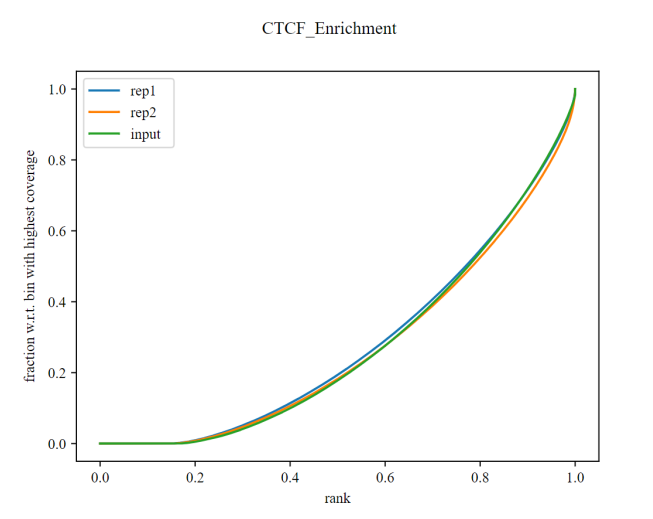
\includegraphics[width=10cm]{figure/chipqc.png}
\end{figure}

理论上,对于没有富集的对照组,其累计曲线应接近与对角线,这与我们的结果符合。对于转录因子的强富集,理想的情况下曲线应该会先缓慢上升,到rank较高的区域后再急剧上升,这表明大量的reads分布在较少的特定窗口中,即蛋白质的结合位点存在显著富集。\par
然而本实验中实验组和对照的累计曲线却相当接近,我们并没有进一步向下探索造成这种现象的原因。


\subsubsection{寻峰}
CTCF是一种转录因子,针对CTCF的ChIP-Seq能够将与之有相互作用的DNA片段富集起来。 Peak calling 是一种ChIP-Seq特有的分析流程,用于鉴定基因组中reads的富集部位。
在ChIP-Seq实验中,比对文件reads的分布是链不对称的:reads以转录因子结合位点为中心,在正义链和反义链各自的5’端形成富集。\par
本流程使用MACS(基于模型的ChIP-Seq分析,Model-based analysis of ChIP-Seq)进行call peak分析。\par
该软件假设DNA上的片段在随机状态下服从泊松分布,macs2根据不满足泊松分布的地方寻找富集点。


\begin{lstlisting}
    ##### step5 call peaks ##########

    echo "call peaks started at $(date)"

    ## 将实验组数据提取出来
    cp rawdata/config rawdata/config2
    cat rawdata/config2 | sed "/input/d" > rawdata/config2

    ## 寻峰,对实验组的所有已经过滤、去重、索引的bam文件寻峰
    cat rawdata/config2 | while read id
    do
    macs2 callpeak -t ./03\_mapping/${id}\_filtered\_dedup.bam \
    -c ./03\_mapping/ctcf\_chip\_input\_filtered\_dedup.bam \
    -f BAMPE -g hs -n CTCF\_ChIP -B -q 0.01 \
    --outdir ./05\_peak\_calling > $./05\_peak\_calling/peak\_calling.log 2>&1
    done
    echo "call peaks finished at $(date)"

    ### 参数说明
    ### -t 处理组的比对文件
    ### -c 对照组的比对文件
    ### -f 输入文件的格式, 设为auto则表示自动识别输入文件的格式;双端测序用BAMPE
    ### -g 有效基因组大小,hs表示人的有效基因组大小,约为2.7E9
    ### -n name string,会成为输出文件的prefix
    ### --outdir 输出文件路径
    ### -B/--BDG 保存堆积对齐片段到bedGraph文件里
    ### -q FDR Cutoff

    ## 备注
    # broad peak常用于组蛋白修饰的peak calling,因为组蛋白修饰往往是一大片;用另外一个程序来call peak
    # narrow peak用于转录因子的peak calling,因此本课题应该使用narrow peak calling。
    # narrowPeak 也可以放进igv里
\end{lstlisting}
macs2的输出结果如下:
\begin{figure}[ht]
    \centering
    \includegraphics[width=7cm]{figure/macs2\_output.PNG}
\end{figure}

NAME\_peaks.xls保存了每个peak的信息:

\begin{enumerate}
    \item chromosome name:染色体名
    \item start position of peak:peak开始的位置
    \item end position of peak:peak结束的位置
    \item length of peak region:peak区域的长度
    \item absolute peak summit position:peak峰出现的位置
    \item pileup height at peak summit:peak峰的堆积高度
    \item -log10(pvalue) for the peak summit (e.g. pvalue =1e-10, then this value should be 10)
    \item fold enrichment for this peak summit against random Poisson distribution with local lambda:相对于随机选取的片段,peak峰高度的变化倍数,即富集倍数
    \item -log10(qvalue) at peak summit
\end{enumerate}
NAME\_peaks.narrowPeak也同样储存了peak的信息:
\begin{enumerate}
    \item 1;染色体号
    \item 2:peak起始位点
    \item 3:结束位点
    \item 4:peak name
    \item 5:int(-10*log10qvalue)
    \item 6:正负链(如果不区分,则记为".")
    \item 7:fold change
    \item 8:-log10pvalue
    \item 9:-log10qvalue
    \item 10:peak的峰相对于peak的位置
\end{enumerate}
NAME\_summits.bed文件记录了所有peak峰的位置和可信度,下游可进一步利用该文件寻找motif\par
NAME\_treat\_pileup.bdg文件用于存放区间的坐标轴信息和相关的评分文件,用于储存稀疏,不连续的数据,并可转化为bigwig文件(二进制,有索引,更高效)\par
NAME\_control\_lambda.bdg文件记录了由对照组中估计得到的局部偏好,可转化为bigwig文件。\par
下载igv软件后,可将排序并索引后的bam文件与narrowPeak文件导入IGV进行可视化查看。
\begin{figure}[ht]
    \centering
    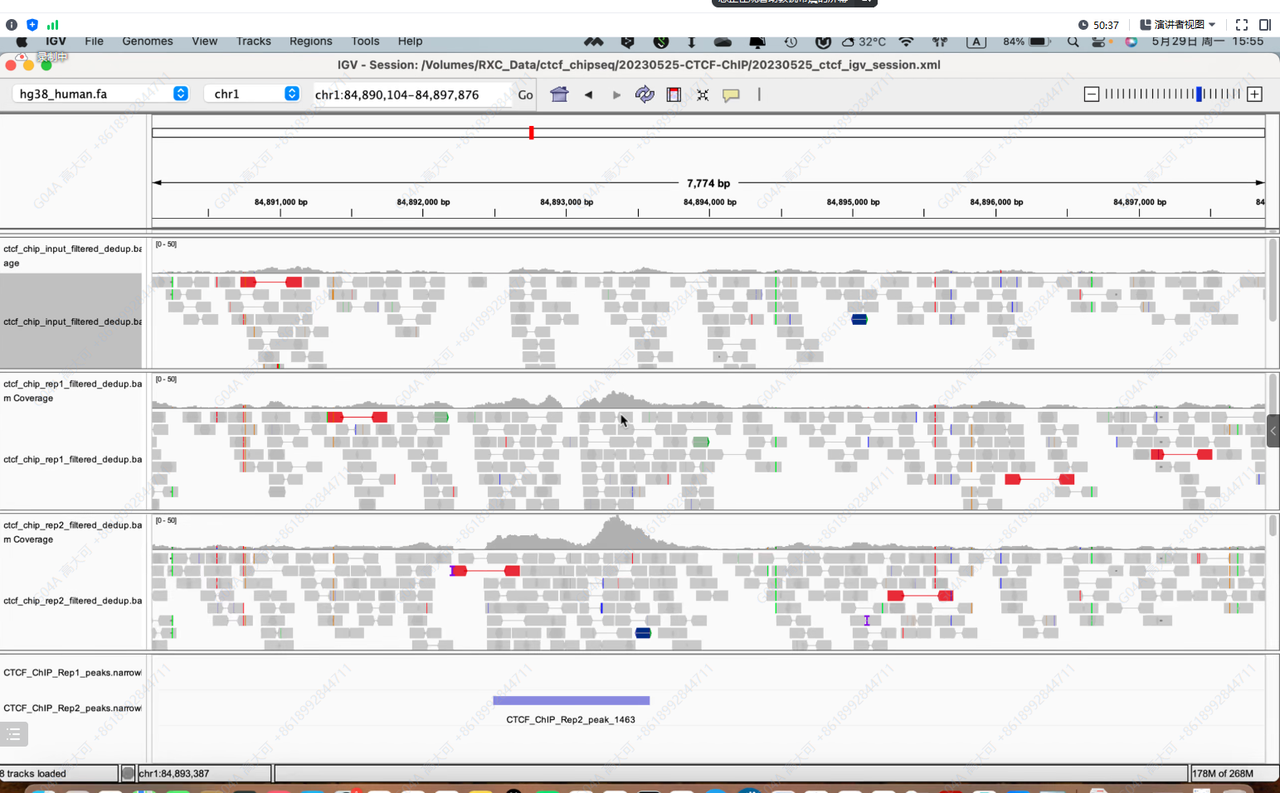
\includegraphics[width=13cm]{figure/igv.png}
\end{figure}

从上图中我们可以可视化地看见narrowpeak的位置,以及那些染色体位置上存在峰的富集。从该图中还能看见部分read太长,只测得了两端(这种情况下macs2会用-f BAMPE进行矫正),部分read太短,二代测序将其测穿,部分位点存在PCR错配或SNP。\par
如果仔细对比rep1和rep2的bam文件在IGV上的可视化图像,可以发现,有的reads的富集在rep2上明显比rep1更多,这可能是因为建库时rep2的富集效果更好,或rep1中某些reads的质量不满足被清洗掉了,或者没有通过假设检验,可以尝试将q值从0.01提高到0.05。\par


\subsubsection{生物学重复的合并}
在进行下游分析时,可以将生物学重复样本合并后进行分析。可以使用IDR软件评估生物学重复样本的相关性,并根据阈值筛选出最终的一组peak,即该软件可从多个生物学重复样本的peak结果中提取高一致性peak区间。\par
使用idr前首先需要对MACS2的结果文件narrowPeak按照p-value排序;排序完成后进行合并。

\begin{lstlisting}
    cat rawdata/config2 | while read id
    do
    sort -k8,8nr ./05\_peak\_calling/${id}\_peak.narrowPeak > ./05\_peak\_calling/${id}\_sorted\_peaks.narrowPeak 
    done

    ### -k8,8 选项使输入文件按其第八列进行排序
    ### -nr 选项指定按整个数字排序(而非一个字符一个字符去比较)

    idr --samples ctcf\_rep1\_sorted\_peaks.narrowPeak ctcf\_rep2\_sorted\_peaks.narrowPeak --input-file-type narrowPeak --rank p.value --output-file sample-idr --plot --log-output-file sample-idr.log
    ### --samples: narrowPeak的输入文件(生物学重复样本)
    ### --input-file-type: 输入文件格式为narrowPeak
    ### --rank p.value: 指定输入文件以p.value排序的
    ### --output-file: 指定输出文件路径
    ### --plot: 输出IDR度量值的结果
\end{lstlisting}

输出文件中,sample-idr是共有peaks的结果输出文件。包含了整合后结果与原本样品1和2的信息。sample-idr.png是结果输出图,描述了两个生物学重复样本中峰的保留情况。\par
在项目的后续分析中没有使用合并的样本,只使用了rep1进行后续下游分析。

\section{ChIP-Seq下游分析}
\subsection{call motif}
使用meme套件进行该任务。\par
可以使用meme-chip寻找motif,并可以详细查看某个转录因子的信息。

\begin{lstlisting}
    mkdir 06\_downstream


    ##### step6. call motif, peak注释和motif search ########

    prefix=CTCF\_ChIP # 该prefix与peak calling的prefix相同
    ### 首先提取用于寻找motif的fasta文件
    ## 取峰值前后100个碱基,第二列-50得到第六列,第三列+49得到第七列,print第1(染色体列),6,7,4列
    awk -v OFS="\t" '{$6=$2-50;$7=$3+49;print $1','$6','$7','$4}' ./04\_peak\_calling/${prefix}\_summits.bed > ./06\_downstream/${prefix}\_motif.bed
    bedtools getfasta -fi /home/wuhangrui/database/ref/hg38/GRCh38.p13.genome.fa -bed ./06\_downstream/${prefix}\_motif.bed > ./06\_downstream/${prefix}\_motif.fasta

    cd /home/wuhangrui/practice/chipseq/06\_downstream

    echo "calling motif started at $(date)"

    mkdir memechip\_out

    meme-chip -db /home/wuhangrui/database/motif\_databases/HUMAN/HOCOMOCOv11\_full\_HUMAN\_mono\_meme\_format.meme -meme-p 10 -dna ${prefix}\_motif.fasta -oc /home/wuhangrui/practice/chipseq/06\_downstream/memechip\_out

    echo "calling motif finished at $(date)"
    cd /home/wuhangrui/practice/chipseq
\end{lstlisting}

可以在输出文件夹下找到输出结果html文件,meme-chip中可以看到软件找出的motif,点击后可在tomtom页面看到该motif的详细信息。\par
注意html结果文件必须和其他meme-chip的输出文件在同一目录下。
\begin{figure}[ht]
    \centering
    \begin{minipage}[c]{0.9\textwidth}
        \centering
        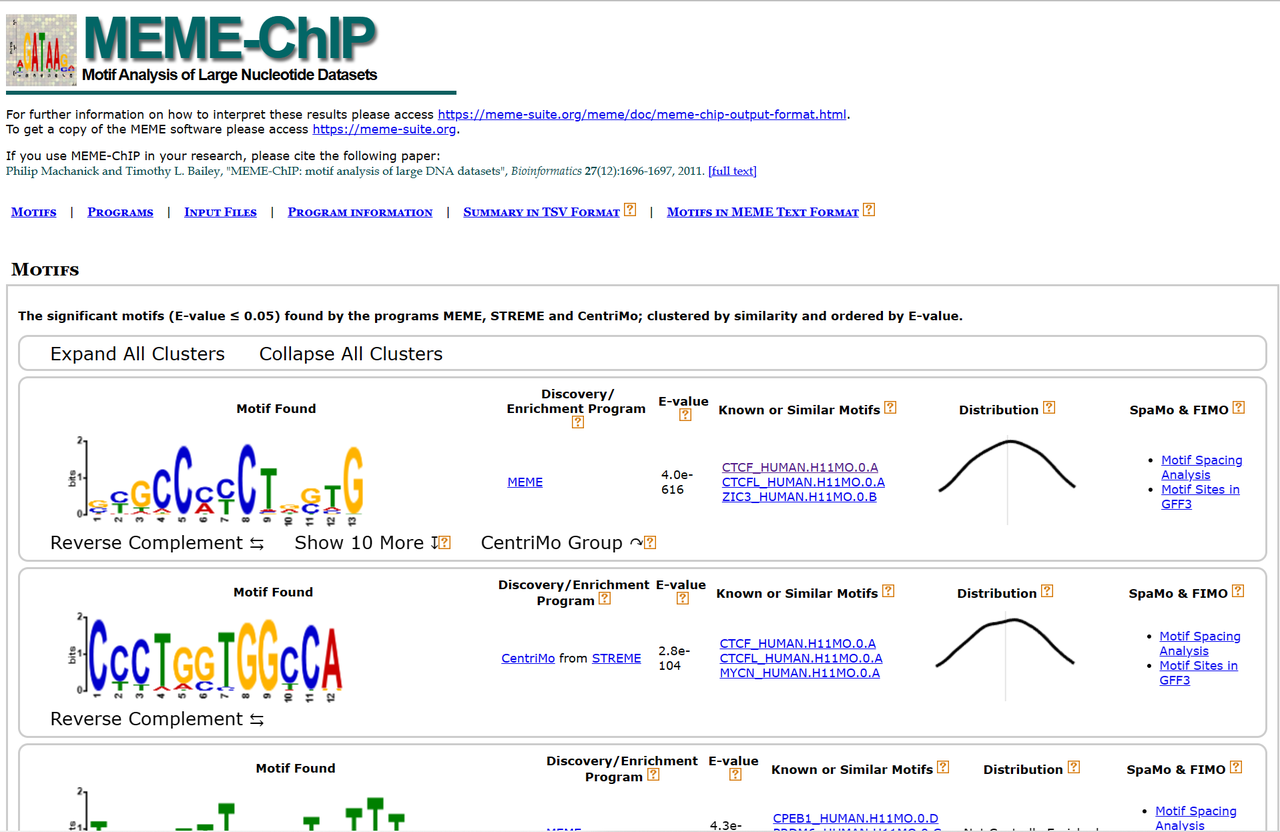
\includegraphics[width=13cm]{figure/memechip.png}
    \end{minipage}

    \begin{minipage}[c]{0.9\textwidth}
        \centering
        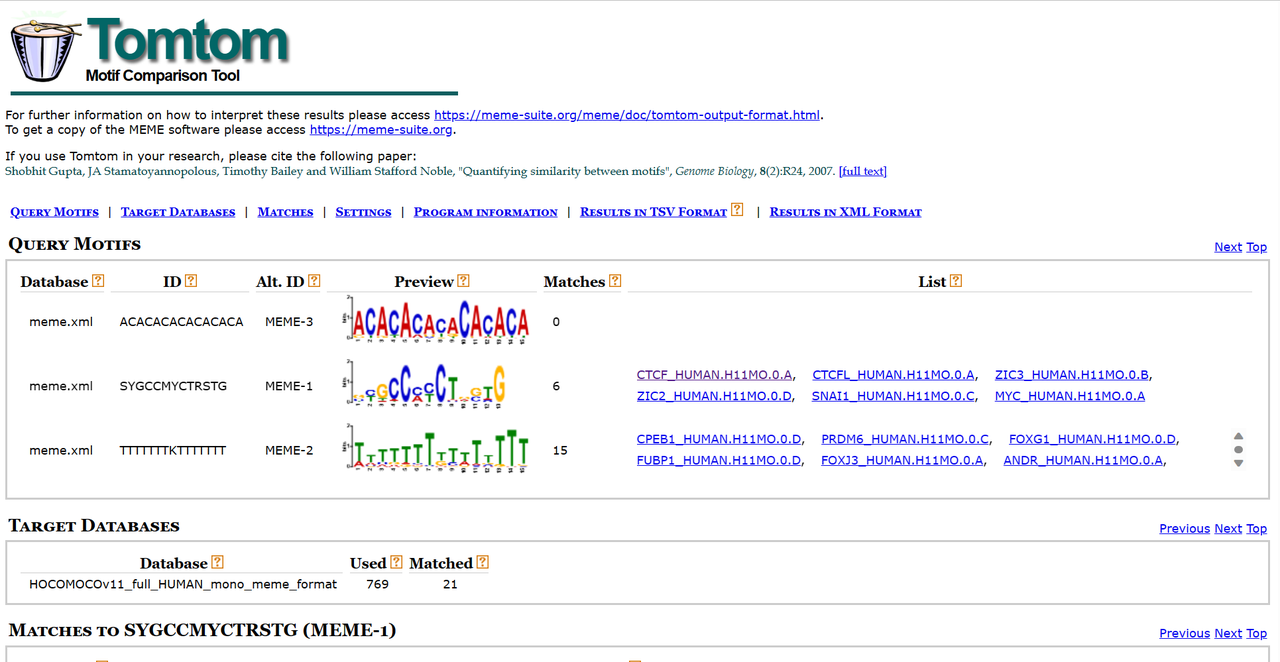
\includegraphics[width=13cm]{figure/tomtom.png}
    \end{minipage}
\end{figure}

\subsubsection{peak注释}
使用Homer进行Peak的注释。Homer包含一个用于峰注释的程序annotatePeaks.pl。它可以将峰与其他附近的基因关联起来。\par
annotatePeaks.pl在默认情况下,会寻找距离peak最近的TSS,并根据TSS所属的基因进行注释。此外该脚本还会根据peak占据的位置,注释其基因组信息
\begin{lstlisting}
    ##### step7. peakannotation ##########
    cd /home/wuhangrui/practice/chipseq/06\_downstream

    echo "peak annotation started at $(date)"
    mkdir peak\_annotation
    annotatePeaks.pl /home/wuhangrui/practice/chipseq/04\_peak\_calling/${prefix}\_peaks.narrowPeak hg38 > peak\_annotation/peak\_annotation.tsv
    echo "peak\_annotation finished at $(date)"

\end{lstlisting}
注释peak得到的信息是表格形式,不方便查看和进一步研究。可以将该输出文件下载到本地用,使用R进行可视化。例如ChIPseeker,GO富集分析,KEGG富集分析等。
该部分是得到的peak注释的进一步分析,和linux本身关系不大,此处省略该部分的代码。可在本组github仓库上寻找相关代码。

\subsection{计算与TSS的共定位情况}
\begin{enumerate}
    \item TSS bed文件可UCSC网站上直接下载,下载选项只需要5’UTR的位置
    \item 需要将索引好的BAM文件转化为bigwig文件
    \item 使用deeptools包下的软件完成该项任务
\end{enumerate}
\begin{lstlisting}
    ##### step8. 不适合看motif的共定位分析 #######
    ##### 8.1 与TSS, TES的共定位情况 #####
    # 使用bamCoverage进行 bam -> bigwig 文件转换(一种压缩方式:将基因组压缩为很多个bin区域)
    # bigwig 文件记录的是“每个碱基”的coverage情况,可以理解为ChIP-Seq的信号
    # 实验组对照组都需要此步骤

    cd /home/wuhangrui/practice/chipseq/06\_downstream
    mkdir co\_location

    # 将input和rep1都进行bam -> bw 文件的转换

    cat /home/wuhangrui/practice/chipseq/rawdata/config | while read id
    do
    bamCoverage --bam /home/wuhangrui/practice/chipseq/03\_mapping/${id}\_filtered\_dedup.bam \
    -o ./co\_location/${id}\_filtered\_dedup.bw \
    --binSize 10 \
    --normalizeUsing RPGC \
    --effectiveGenomeSize 2913022398 \
    --extendReads \
    -p 10
    done

    ### --bam输入的bam文件
    ### -o 输出的bigwig文件
    ### --binSize 计算coverage时的bin的大小
    ### --normalizeUsing 选择normalization的方法 RPGC按照bin和测序量大小归一化
    ### --effectiveGenomesize 如果需要normalization则需有设置有效基因组大小
    ### --extendReads 设置该值以拓展reads的长度,以计算出用于测序的DNA片段的长度;pair-end的测序可以自动估计DNA片段的长度
    ### -p 使用的线程数


    ##### 与其他区域的共定位情况(高甲基化区域,低甲基化区域,5'UTR,3'UTR等)
    # 使用“computeMatrix”计算指定位置的信号矩阵
    cd /home/wuhangrui/practice/chipseq/06\_downstream

    computeMatrix reference-point \
    -S ./co\_location/ctcf\_chip\_input\_filtered\_dedup.bw ./co\_location/ctcf\_chip\_rep1\_filtered\_dedup.bw ./co\_location/ctcf\_chip\_rep2\_filtered\_dedup.bw \
    -R /home/wuhangrui/database/ref/hg38/uscs\_refseq.bed \
    -a 2500 -b 2500 \
    --samplesLabel input ctcf\_rep1 ctcf\_rep2 \
    --sortRegions descend \
    -o ./co\_location/Rep1\_Input\_TSS\_Matrix.gz \
    -p 10 > computeMatrix\_input.log 2>&1

    # 使用reference-point模式,reference位点为TSS位置
    ### -S 输入的bigwig文件
    ### -R 记录reference位点信息的bed文件
    ### -a 起始位点上游的距离
    ### -b 起始位点下游的距离
    ### --sortRegions 在矩阵中,信号按什么顺序排列?
    ### --samplesLabel 在矩阵中,样品如何命名
    ### -o 输出的矩阵名
    ### -p 线程数
    ### 如果热图中出现黑色条状色块,可以尝试增加--missingDataAsZero选项

    # 使用plotHeatmap作图
    cd /home/wuhangrui/practice/chipseq/06\_downstream
    plotHeatmap -m ./co\_location/Rep1\_Input\_TSS\_Matrix.gz \
    -out ./co\_location/Rep1\_Input\_TSS\_Matrix.svg \
    --plotFileFormat svg --yAxisLabel RPGC --regionsLabel all\_tss \
    --legendLocation none

    ### -m 输入的矩阵文件
    ### -out 输出的图片文件
    ### --plotFileFormat 指定输出文件的格式
    ### --yAxisLabel 指定y轴标签
\end{lstlisting}

\begin{figure}[ht]
    \centering
    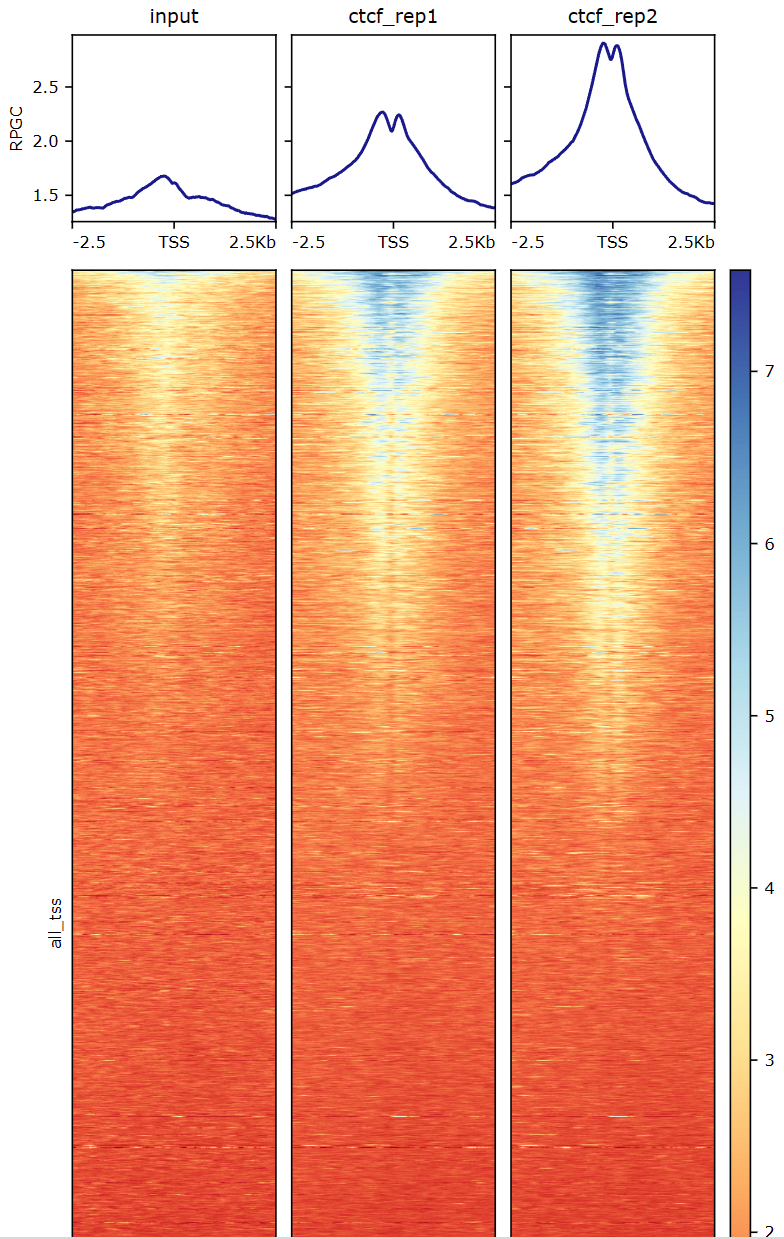
\includegraphics[width=13cm]{figure/heatmap.png}
    \caption{热图}
    \label{heatmap}
\end{figure}

如图\ref{heatmap},可见处理组在TSS上有非常明显的富集,且呈现双峰模式。颜色表示reads密度。               % ChIP-seq 
\chapter{RNA Seq}

\section{软件的安装}
主要使用到了cutadapt、STAR、fastqc、stringtie,首先使用在conda config中添加bioconda,再创建一个环境,添加会使用到的各种包。
\begin{lstlisting}
    conda config --add channels bioconda
    conda create -n rnaseq
    conda activate rnaseq
    conda install cutadapt STAR fastqc stringtie
\end{lstlisting}

\begin{figure}[ht]
    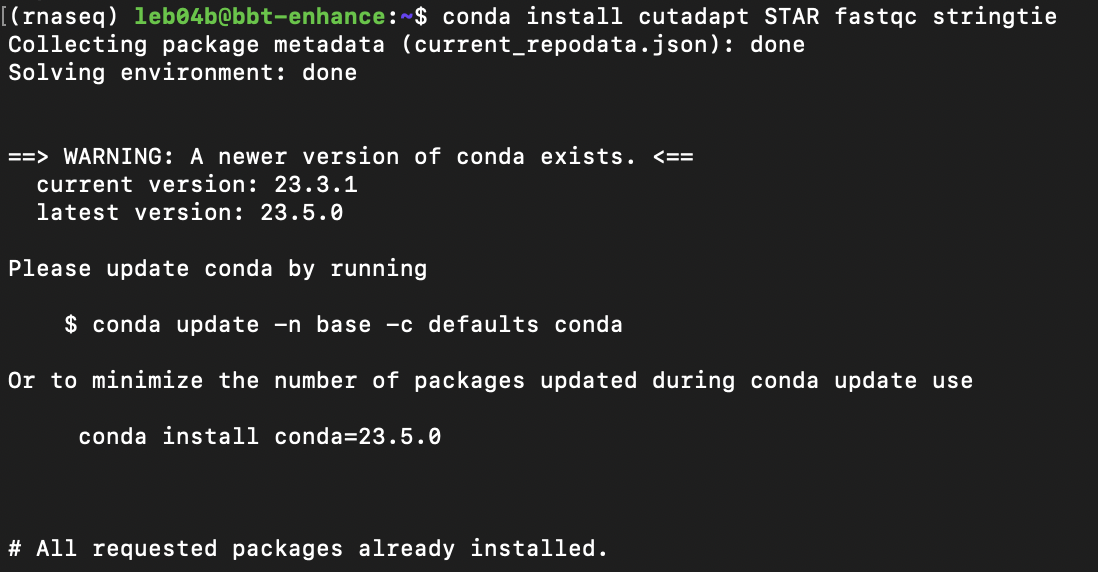
\includegraphics[width=13cm]{image/rnaseq/package.PNG}
\end{figure}

\section{RNA-seq上游分析}
RNA-seq上游分析与ChIP-Seq类似,参见。故此处仅简单提及。

\subsection{质控}
原始数据为fastq.qz文件,一般是双端配套的比对结果,有两个文件
使用fastqc进行质控,最后得到两个文件,其中一个为html文件,可用网页浏览,也可以在VSCode中安装html插件查看。

\begin{figure}[ht]
    \begin{minipage}[C]{0.9\textwidth}
        \centering
        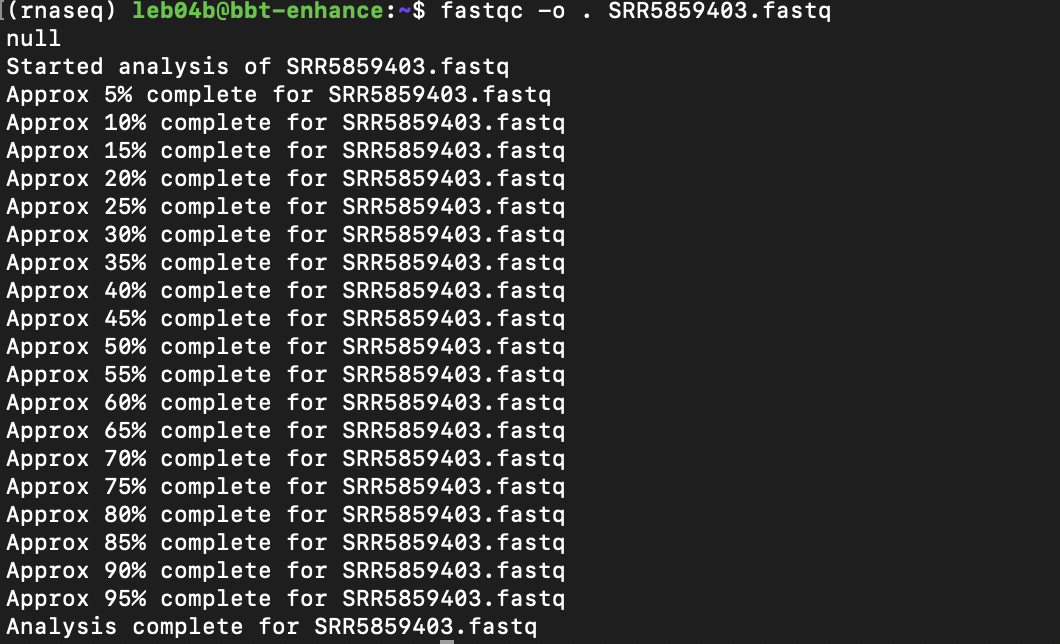
\includegraphics[width=13cm]{image/rnaseq/qc.PNG}
    \end{minipage}

    \begin{minipage}[C]{0.9\textwidth}
        \centering
        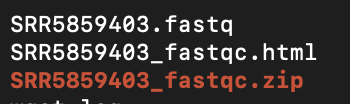
\includegraphics[width=5cm]{image/rnaseq/qcfile.PNG}
    \end{minipage}
\end{figure}

\subsection{使用cutadapt去接头}

\subsection{比对}
下载参考基因组,star建立索引。比对后,可以得到bam、log、log out、log final out文件

\subsection{定量}
使用stringtie,输入bam文件,得到gtf文件(包含基因、数量)

使用stringtie的自带脚本prepDE.py运行得到的gtf文件得到表达矩阵csv文件

\section{RNA-seq下游分析}
表达矩阵每一列是一个样本,每一行是一个基因。(注意基因 symbol 和ensembl id 的转换)

clusterprofiler包中的bitr函数可以进行symbol到ensembl id的转化

\subsubsection{差异表达基因分析(在R的环境下运行)}

引入相应的包
\begin{lstlisting}
    library(tidyverse)
    library(pheatmap)
    library(DESeq2)
    library(readxl)
    library(EnhancedVolcano)
    library(clusterProfiler)
    library(org.Hs.eg.db)

    #加载常用的包
    #如未下载,可使用类似代码进行安装
    #
    #if (!require("BiocManager", quietly = TRUE))
    #  install.packages("BiocManager")
    #BiocManager::install("EnhancedVolcano")
    #安装后,必须使用library命令激活

\begin{lstlisting}
    getwd()
    setwd('leb/rnaseq')
    #切换工作目录
\end{lstlisting}

读取生成的文件
\begin{lstlisting}
    rna_seq <- read_excel(
    "RNAseq.xlsx",
    sheet = "Readcounts"
    )
    #读入excel文件
    #注意!数据类型未tibble,不是data.frame!
\end{lstlisting}

进行id转化
\begin{lstlisting}
    genid <- bitr(rna_seq$Geneid, fromType = "ENSEMBL", toType = "SYMBOL",
        OrgDb = org.Hs.eg.db)
        # org.Hs.eg.db是一个homo sapiens数据库,根据该数据库中的注释进行id转换

\end{lstlisting}

整理数据格式
\begin{lstlisting}
    rna_seq <- rna_seq %>%
    mutate(Gene = ...1) %>%
    dplyr::select(-...1) %>%
    group_by(Gene) %>%
    summarise_all(sum) %>% # 这里的sum是对每一列进行求和,其实这个矩阵应该是已经整理好的不用。
    as.data.frame()

    # 使用管道符

    rownames(rna_seq) <- rna_seq$Gene
    rna_seq <- rna_seq[, -1] # remove Gene column
    print(head(rna_seq))
    rna_seq <- rna_seq[-c(1:20), ] # 去掉前20行,这里面是一些不是基因的东西
    rna_seq <- rna_seq[rowSums(rna_seq) >= 10, ] # 去掉在所有样本里面表达量小于10的基因
\end{lstlisting}

直接生成图片的时候要把plot框调到合适大小
\begin{lstlisting}
    > biplot(p)
    Error in grid.Call(C_convert, x, as.integer(whatfrom), as.integer(whatto),  :
    Viewport has zero dimension(s)
\end{lstlisting}

\subsubsection{数据质控}
Plotcount 可以查看目标基因的表达情况
\begin{lstlisting}
    plotCounts(dds, gene = "RBMX", intgroup = "type")
\end{lstlisting}

\begin{figure}[ht]
    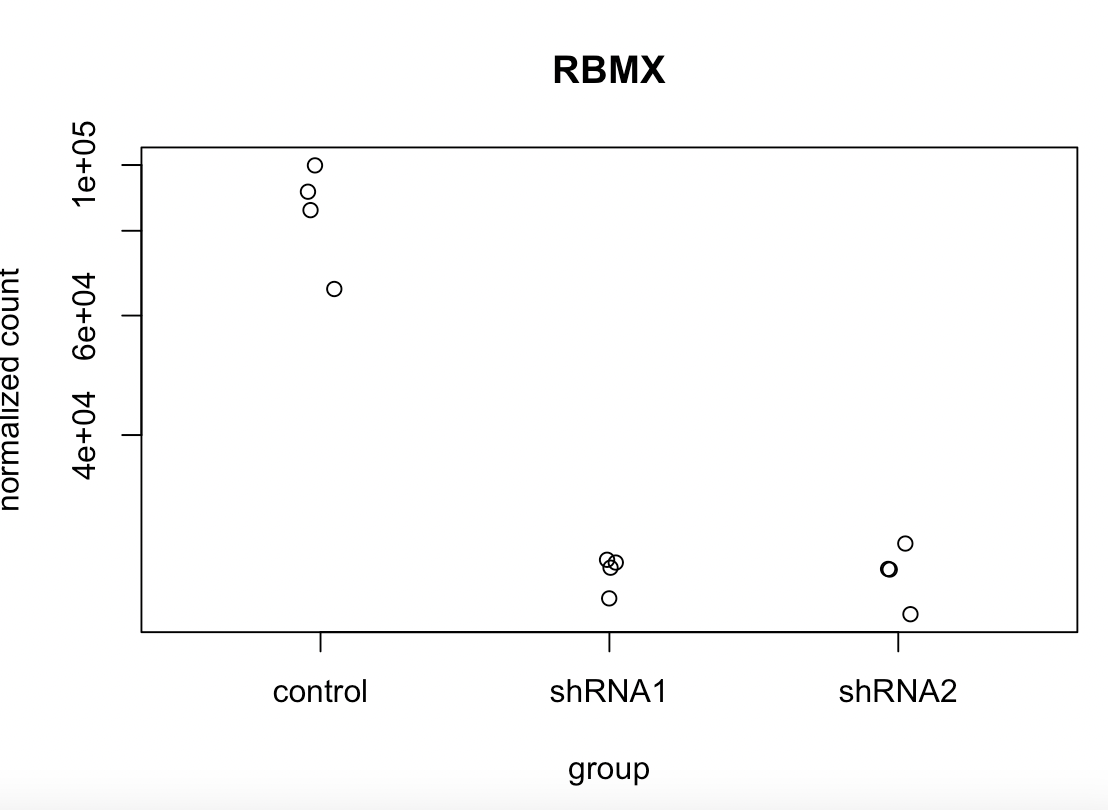
\includegraphics[width=10cm]{image/rnaseq/qc2.png}
\end{figure}

使用PCA降维聚类
\begin{lstlisting}
    library(PCAtools)
    vst <- rna_seq
    meta <- data.frame(row.names = colnames(rna_seq), type = id$type)
    p <- pca(vst, metadata=meta, removeVar = 0.05)
    biplot(p)
\end{lstlisting}

\begin{figure}[ht]
    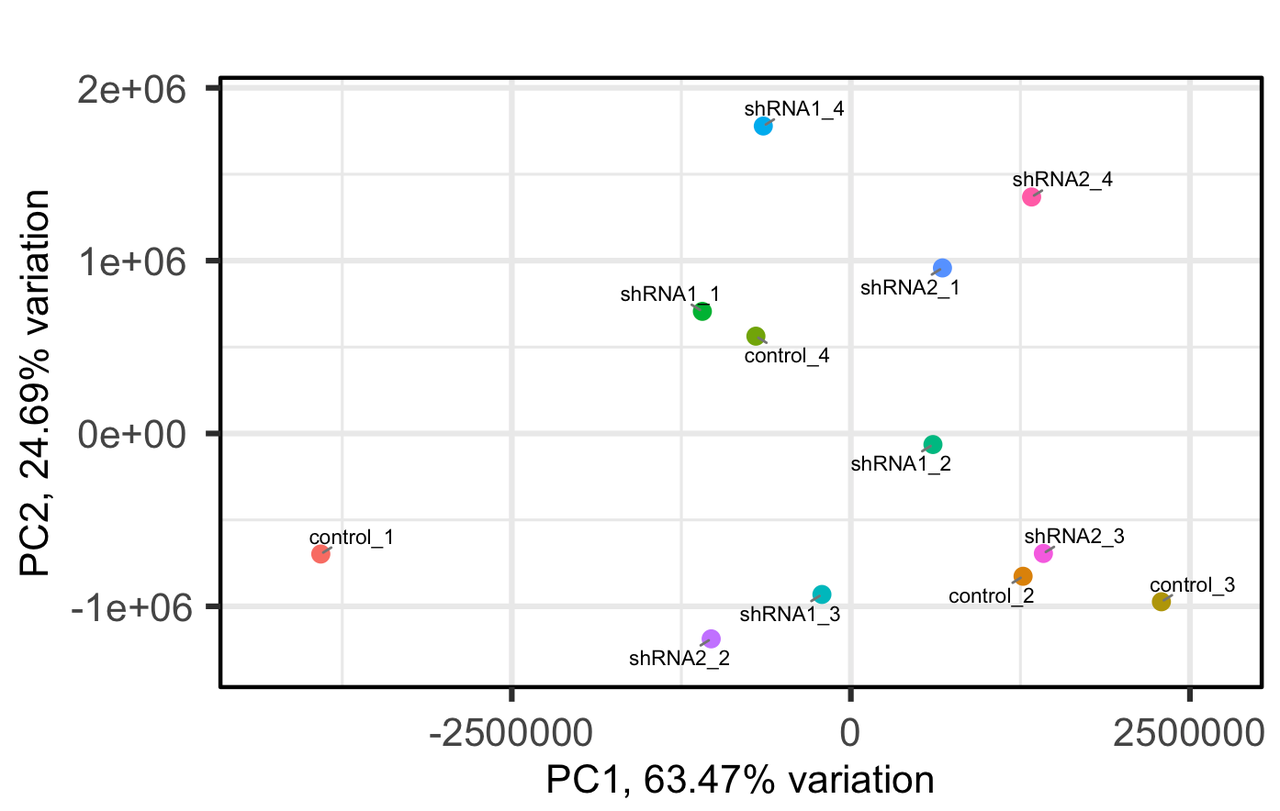
\includegraphics[width=13cm]{image/rnaseq/pca.png}
\end{figure}

火山图的绘制,如图\ref{volcano}。
\begin{lstlisting}
    res1 <- results(dds, name="type_shRNA1_vs_control")
    res2 <- results(dds, name="type_shRNA2_vs_control")
    EnhancedVolcano(res1,
    lab = rownames(res1),
    x = "log2FoldChange",
    y = "pvalue"
    )
    EnhancedVolcano(res2,
    lab = rownames(res2),
    x = "log2FoldChange",
    y = "pvalue"
    )
\end{lstlisting}

\begin{figure}[ht]
    \centering
    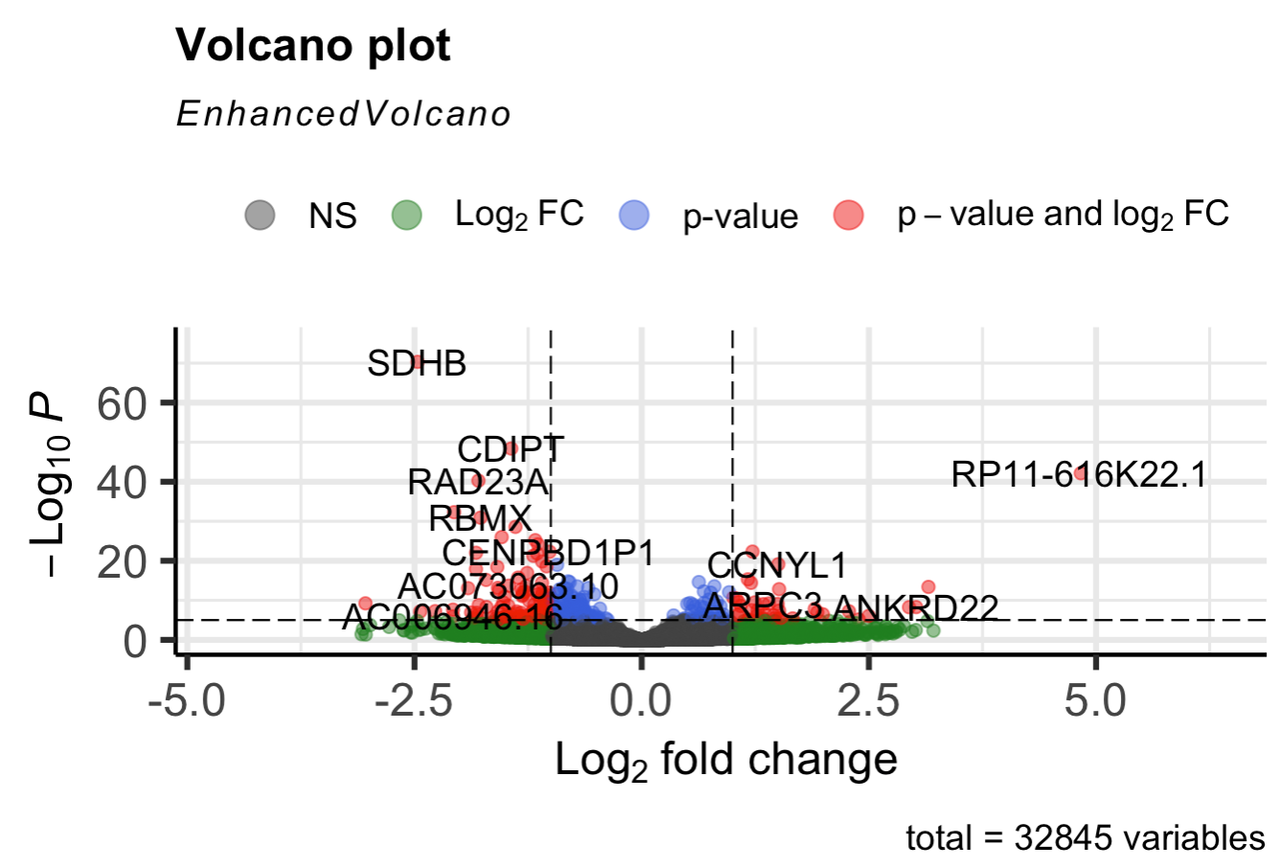
\includegraphics[width=13cm]{image/rnaseq/volcano.png}
    \caption{火山图}
    \label{volcano}
\end{figure}

pheatmap对差异基因绘制热图,如图\ref{dif}。
\begin{lstlisting}
    res_filtered <- res2 %>%
    as.data.frame() %>%
    rownames_to_column("Gene") %>%
    filter(padj < 0.05 & abs(log2FoldChange) > 1)
    dim(res_filtered)
    print(head(res_filtered))
    differential_genes <- res_filtered$Gene
    diff_matrix <- rna_seq[sample(differential_genes, 50), ]
    RBMX <- rna_seq["RBMX",]
    diff_matrix <- rbind(diff_matrix, RBMX)
    pheatmap(diff_matrix, scale = "row")
    ggsave("heatmap.png", width = 10, height = 10)
\end{lstlisting}

\begin{figure}[ht]
    \centering
    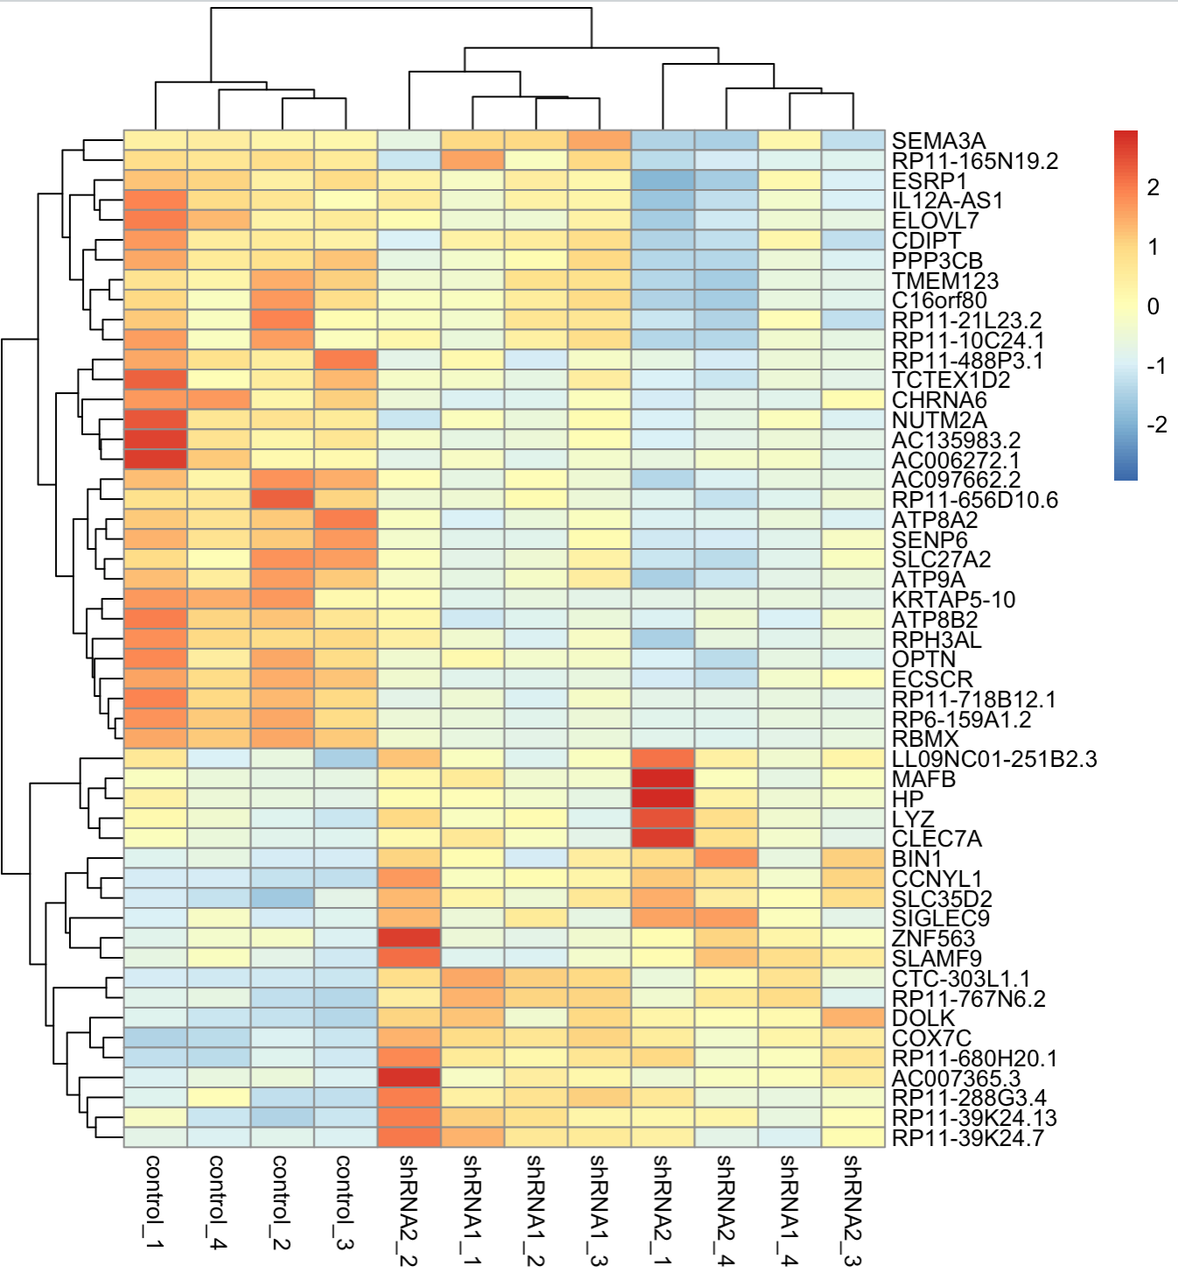
\includegraphics[width=10cm]{image/rnaseq/heatmap.png}
    \caption{基因差异表达结果}
    \label{dif}
\end{figure}

\subsubsection{GO富集分析}
使用clusterprofile包可以进行go富集分析,如图\ref{go}。
\begin{lstlisting}
    library(clusterProfiler)
    library(org.Hs.eg.db)
    #gene ontology
    go_bp <- enrichGO(gene = differential_genes,
    OrgDb = org.Hs.eg.db,
    keyType = "SYMBOL",
    ont = "BP", # BP: biological process, MF: molecular function, CC: celluar component, ALL
    pAdjustMethod = "BH",
    pvalueCutoff = 0.05,
    qvalueCutoff = 0.05)
    dotplot(go_bp, title = "GO Biological Pathway", showCategory = 10)
\end{lstlisting}

\begin{figure}[ht]
    \centering
    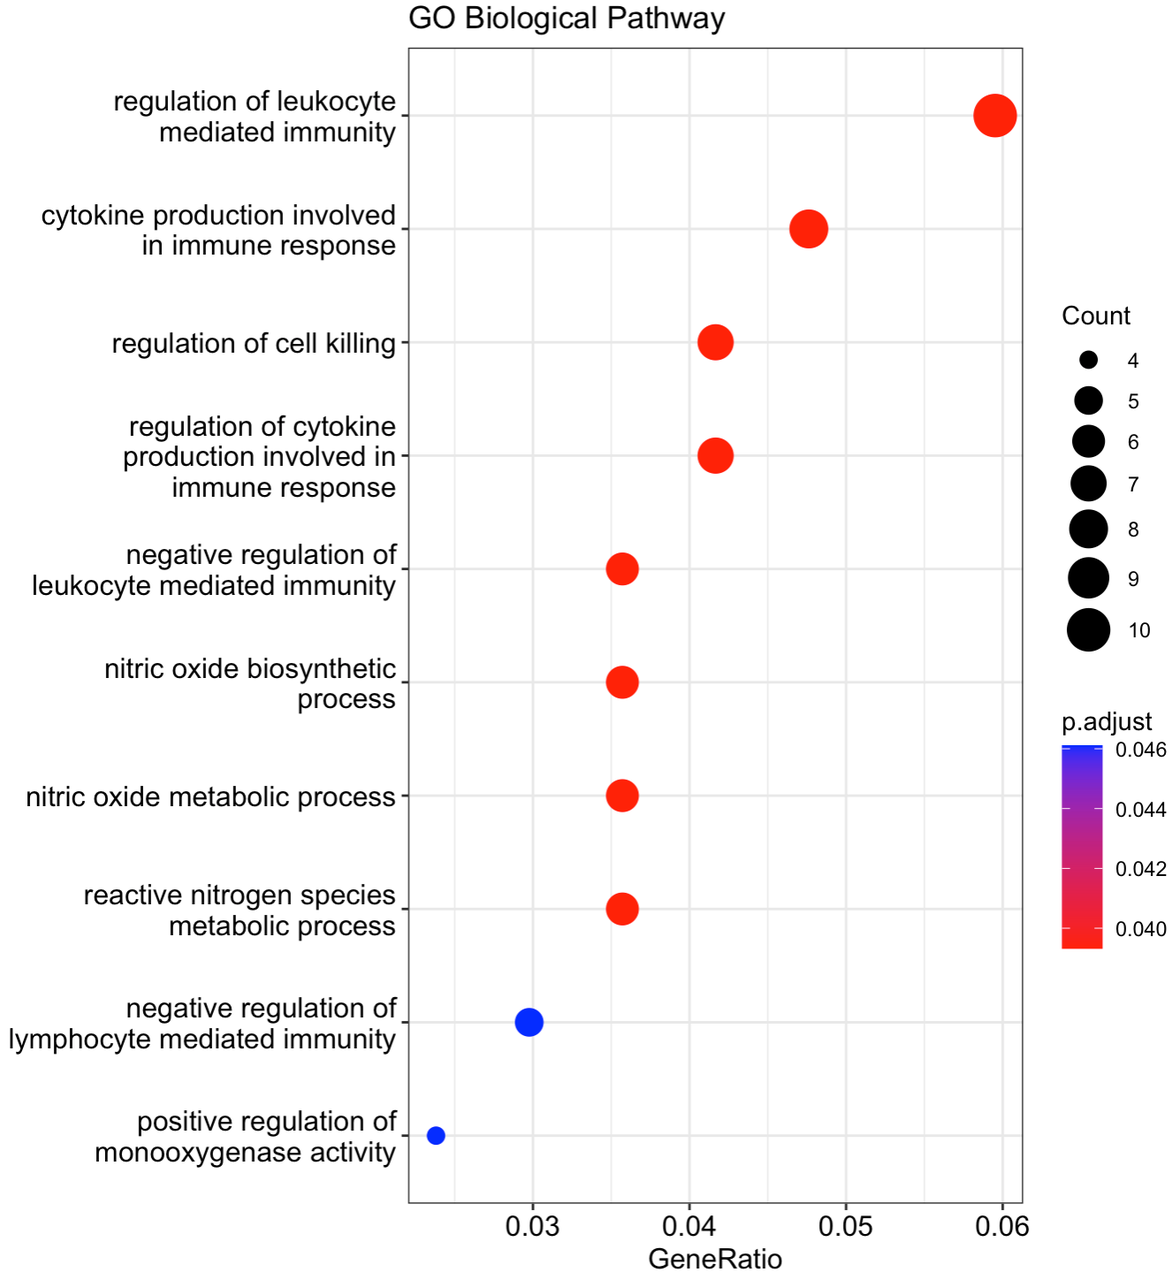
\includegraphics[width=10cm]{image/rnaseq/go.png}
    \caption{GO富集分析结果}
    \label{go}
\end{figure}               % RNA-seq

\chapter*{致谢}

首先,非常感谢罗静初老师。
罗老师非常认真地规划了这门课程,从课前预习部分、课上理论与实践、课后讨论,罗老师都会通过邮件和大家交流。

饶希晨师兄作为助教,在组织课程中投入了很多的时间与精力。
在课程中,老师还邀请了吕钰麟、颜林林等学长为我们讲解相应部分的知识,
也邀请了易鼎程、王沛宇、张任子墨等同学分享他们的经验。

罗老师为我们推荐的\href{http://abc.gao-lab.org/}{Applied Bioinformatics Course}中包含大量的参考资料,包括生信分析常见软件、文献与常用的数据库网站,是非常实用的网站。

感谢教学中心为课程提供的教学服务器、高性能服务器,
这保证我们在课程进行时能够顺利地同步运行代码。

在这门课程中,我们不仅了解、学习了生信分析相关的原理与软件,还学习了撰写代码的逻辑。

对于能够选上这门课程,我们感到十分幸运。         % 致谢

\appendix
\chapter{环境配置}

\section{Linux环境配置}
Windows和MacOS是当前最流行的两个操作系统,其中,MacOS是类Unix系统,与Linux共享编程语言,因此你可以在Terminal中直接使用Linux相关指令。如果你是Windows系统,你需要安装Linux子系统或虚拟机。

\subsection{Windows Subsystem for Linux, WSL}
WSL是Windows Subsystem for Linux的缩写,是一个在Windows 10上能够运行原生Linux二进制可执行文件(ELF格式)的兼容层。它是由微软与Canonical公司合作开发,其目标是使纯正的Ubuntu、Debian等映像能下载和解压到用户的本地计算机,并且映像内的工具和实用工具能在此子系统上原生运行。

WSL提供了一个完整的Linux内核,但它不是一个虚拟机。相反,WSL提供了一个Linux系统调用兼容层,以便可以在Windows上运行原生Linux二进制文件。这意味着您可以在Windows上运行Linux命令行工具、脚本和应用程序,而无需使用虚拟机或双引导设置。

\subsection{WSL配置}\cite{wsl}
Windows提供了方便的WSL配置流程,在管理员模式下打开 PowerShell 或 Windows 命令提示符,方法是右键单击并选择“以管理员身份运行”,输入 \lstinline{wsl --install} 命令,然后重启计算机,即可完成安装。

\begin{lstlisting}
    wsl --install
\end{lstlisting}

若要更改安装的发行版,输入\lstinline{wsl --install -d <Distribution Name>}。 将\lstinline{<Distribution Name>}替换为要安装的发行版的名称。

若要查看可通过在线商店下载的可用 Linux 发行版列表,可输入:\lstinline{wsl --list --online} 或 \lstinline{wsl -l -o}。

安装完成后即可在终端(terminal)看到Ubuntu或直接在应用列表中搜索到Ubuntu,如图\ref{ubuntu}所示:

\begin{figure}[ht]
    \centering
    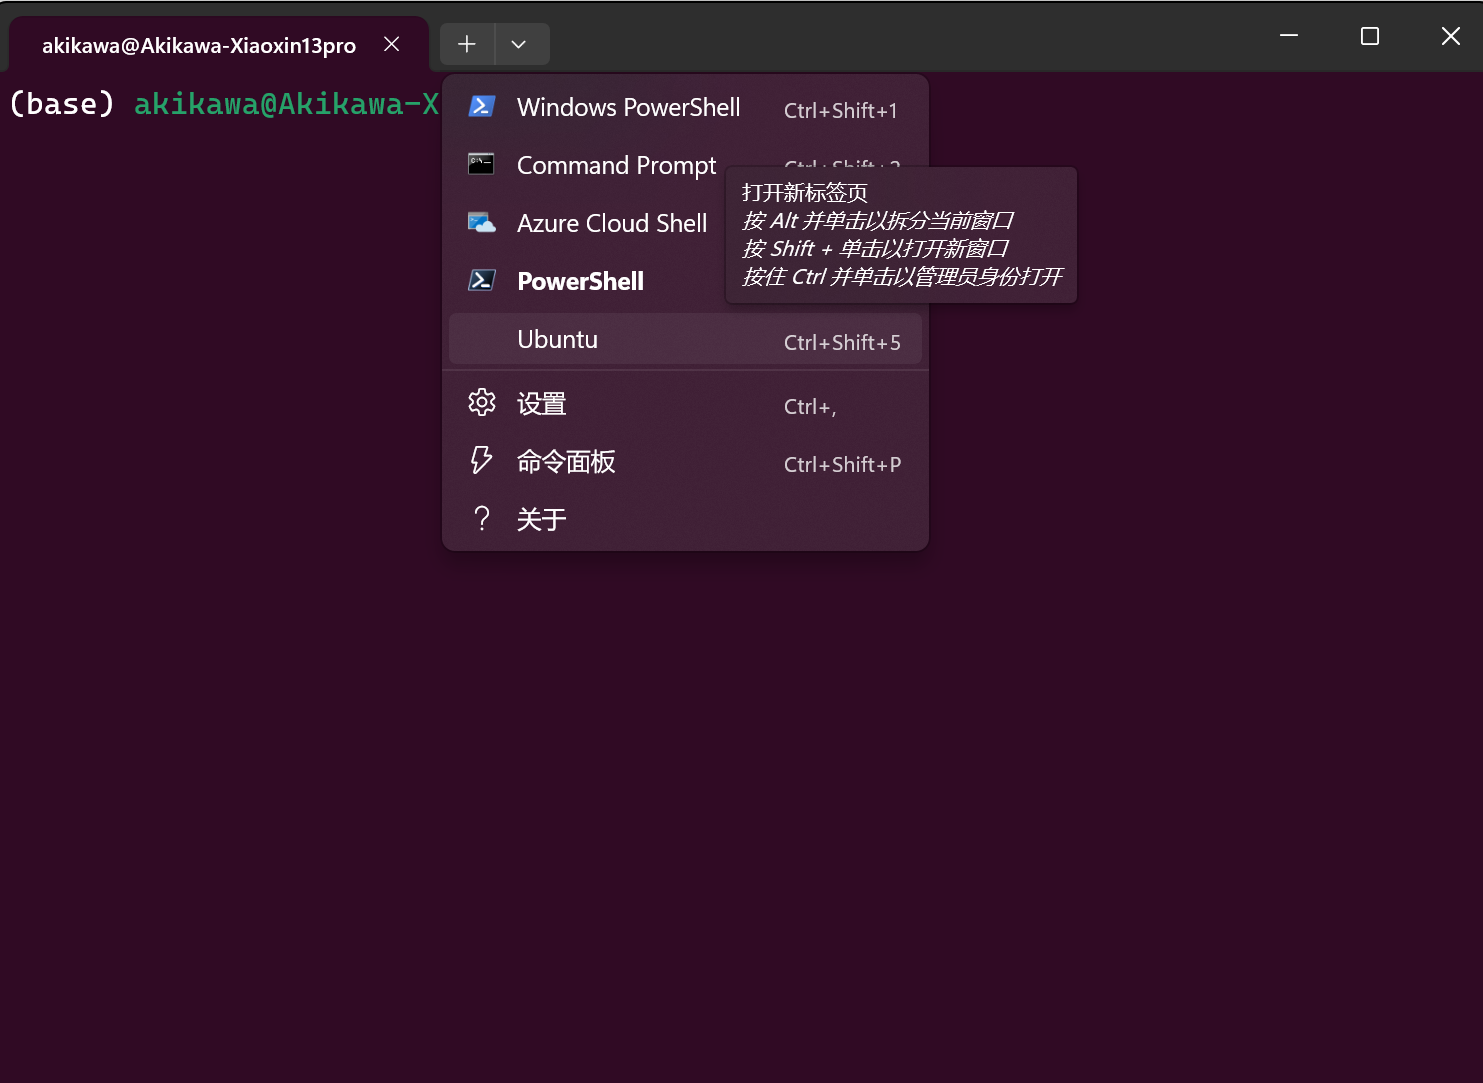
\includegraphics[width=13cm]{image/env/wsl-ubuntu.png}
    \caption{在终端中打开wsl}
    \label{ubuntu}
\end{figure}

\section{conda:环境管理系统}
Conda 是一个开源的包管理系统和环境管理系统,可在 Windows、macOS 和 Linux 上运行。 Conda 可快速安装、运行和更新包及其依赖项。 Conda 可以轻松地在计算机上创建、保存、加载和切换环境。 它是为 Python 程序而创造的,但它可以打包和分发任何语言的软件。

\subsection{conda安装}
conda分为anaconda和miniconda两种,前者包含一个基础的python环境,其中预装了常用的包;而后者较为精简,后续所有需要的东西可自行安装。这里展示miniconda的下载和安装过程,anaconda类似,只需要更改下载链接即可。

\subsubsection{conda下载}
以下是使用wget通过conda官网或者清华镜像源下载miniconda的代码,根据需要选择其一即可。
\begin{lstlisting}
    wget -c https://repo.continuum.io/miniconda/Miniconda3-latest-Linux-x86_64.sh
    wget -c https://mirrors.bfsu.edu.cn/anaconda/miniconda/Miniconda3-latest-Linux-x86_64.sh        #清华的镜像源latest的版本会一直更新到最新的版本
\end{lstlisting}

其中,-c表示断点续传。一般来说,如果没有VPN,清华镜像源下载速度较快,更为推荐。

\subsection{conda安装}
使用bash运行下载好的\lstinline{Miniconda3-latest-Linux-x86_64.sh}文件,如下:
\begin{lstlisting}
    bash Miniconda3-latest-Linux-x86_64.sh              #运行.sh 
\end{lstlisting}

安装过程中某一步会让你指定安装路径,如果有特殊需要可以改为你想安装到的路径(我将linux上安装的软件都放入了\lstinline{~/.app}中),否则全部选择yes即可。

\subsection{conda运行}
安装完成后,在终端中直接运行conda是无法启动的,你可以在\lstinline{~/.bashrc}中看见conda的路径,需要运行.bashrc文件进行初始化后方可进入conda环境,\lstinline{.bashrc}文件内容如下图:

\begin{figure}[ht]
    \centering
    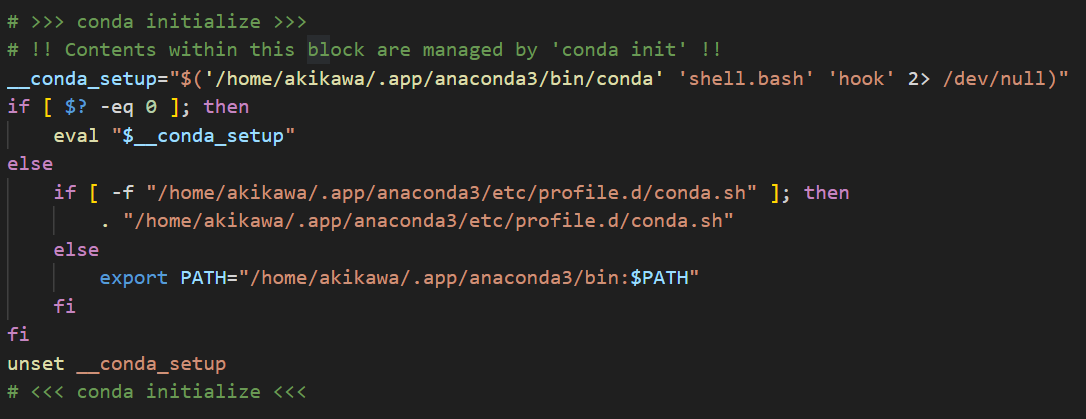
\includegraphics[width=13cm]{image/env/conda-initiate.png}
    \caption{.bashrc文件中的conda初始化部分}
\end{figure}

\subsection{环境}
环境是 conda 的重要概念,conda 可以创建各种环境,每个环境可以指定具体的 python 版本,可以在指定的环境下安装管理自己所需的包,并且环境之间相互隔离,互相不影响,类似命名空间的作用,对于不同需求场景下可以进行环境的自由切换,以下是与环境相关的一些简单命令,可在终端中打开Ubuntu后输入以下命令执行对应操作。
\begin{lstlisting}
    # 创建环境
    conda create -n forfun python=3.6
    # 列出所有环境
    conda env list
    # 删除环境
    conda env remove -n forfun
    # 激活环境
    source activate forfun
    # 退出环境
    source deactivate
\end{lstlisting}

在某个环境下,可以通过下述命令管理包
\begin{lstlisting}
    # 检索可以下载的包
    conda search numpy
    # 下载包
    conda install numpy  
    # 移除包
    conda remove numpy  
    # 列出所有安装包
    conda list
\end{lstlisting}


\section{VSCode:轻量化集成代码编辑器}
VSCode 全称 Visual Studio Code,是微软出的一款轻量代码编辑器,免费、开源而且功能强大。它支持几乎所有主流的程序语言的语法高亮、智能代码补全、自定义热键、括号匹配、代码片段、代码对比 Diff、GIT 等特性,支持插件扩展,并针对网页开发和云端应用开发做了优化。软件跨平台支持 Win、Mac 以及 Linux。

\subsection{VSCode安装及中文环境配置}
打开 \href{https://code.visualstudio.com/}{VSCode官网},点击下载链接即可s下载安装。下载简体中文插件后即可将语言切换为中文。此后,如需配置对应的环境,如Python、R、Latex环境,只需下载主程序后\footnote{因为本质上VSCode只是一个壳,和记事本类似,程序的运行是在对应终端中进行的}在VSCode中安装对应的包即可。

\begin{remark}
    VSCode除了各类代码,还可以方便地打开xml、csv、xlsx、docx、tif、html、svg等常见文件,只要安装对应的插件即可;也可以直接对文本文件进行编辑,因而VSCode为没有图形化界面的WSL增添了许多便利。
\end{remark}

\subsection{VSCode连接WSL、SSH}
安装好WSL后,在VSCode左侧侧边栏的Remote Explorer分区,你可以在上方选择WSL Target直接连接到子系统,方便完成文本编辑,文件预览,文件传输等功能(可将Windows上文件直接拖动到VSCode的资源管理器中完成上传,将WSL上文件通过右键点击完成下载)等功能



\subsection{在VSCode上通过SSH连接远程Linux服务器}
\subsubsection{在VSCode中配置SSH}
\begin{quotation}
    本部分参考CSDN上部分文章\cite{ssh},结合我们自身配置过程书写而成。
\end{quotation}
在win10中安装open-SSH客户端,可使用“应用与程序”或“windows power shell”,如图\ref{win-ssh}。
\begin{figure}[ht]
    \centering
    \begin{minipage}[c]{0.45\textwidth}
        
\includegraphics[width=\textwidth]{image/env/win-ssh.png}
    \end{minipage}
    \begin{minipage}[c]{0.45\textwidth}
        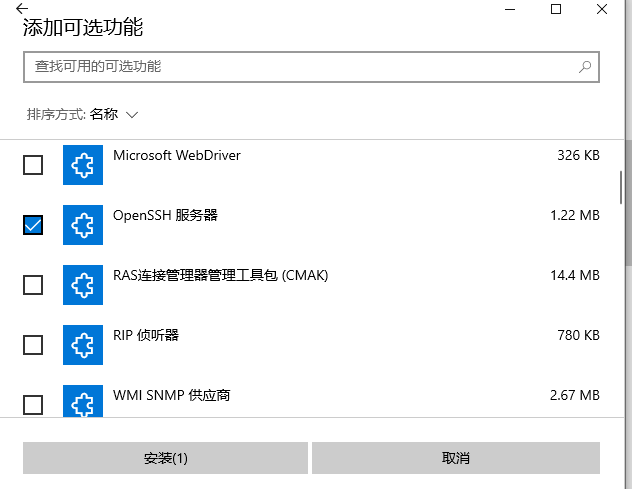
\includegraphics[width=\textwidth]{image/env/win-ssh2.png}
    \end{minipage}

    \caption{Win10中安装OpenSSH}
    \label{win-ssh}
\end{figure}

在vs-code的extension中搜索remote-ssh并安装
\begin{figure}[ht]
    \centering
    \includegraphics[width=13cm]{image/env/vsc-plugin.png}
\end{figure}

配置.config文件
\begin{figure}[ht]
    \centering
    \begin{minipage}[c]{0.65\textwidth}
        \includegraphics[width=\textwidth]{image/env/vs-ssh-config.png}
    \end{minipage}
    \begin{minipage}[c]{0.3\textwidth}
        \includegraphics[width=\textwidth]{image/env/vs-remote.png}
    \end{minipage}
    \caption{VSCode中配置SSH远程连接}
    \label{vs-ssh}
\end{figure}

\begin{lstlisting}
    Host LEB
    HostName 117.78.18.116
    User leb4c

    Host LEB_enhanced
    HostName 114.115.164.221
    User leb04c
\end{lstlisting}

其中,Host、HostName和User分别表示你希望显示在本地的服务器名称,服务器SSH地址和你在服务器上登录的用户名。保存后可直接点击列表内的服务器登录,如图\ref{vs-ssh}右所示。

右键添加扩展设置。
\begin{figure}[ht]
    \centering
    \includegraphics[width=13cm]{image/env/vs-ssh-plugin-set.png}
\end{figure}

勾选首选项中显示登录窗口,以输入密码
\begin{figure}[ht]
    \centering
    \includegraphics[width=13cm]{image/env/vs-remote-show-login.png}
\end{figure}

在VSCode中登录并在提示后输入密码,如图\ref{login}。

\begin{figure}[ht]
    \centering
    \begin{minipage}[c]{0.9\textwidth}
        \centering
        \includegraphics[width=13cm]{image/env/ssh-login.png}
    \end{minipage}

    \begin{minipage}[c]{0.9\textwidth}
        \centering
        \includegraphics[width=13cm]{image/env/pswd.png}
    \end{minipage}
    \caption{VSCode中登录}
    \label{login}
\end{figure}

可以通过VSCode清晰展示各个文件、路径,可在展示termial的同时修改文件内容,如图\ref{vsc-page}。
\begin{figure}[ht]
    \centering
    \includegraphics[width=13.5cm]{image/env/vs-remote-show.png}
    \caption{VSCode连接服务器后的页面}
    \label{vsc-page}
\end{figure}

\subsubsection{配置SSH免密码登录}
\begin{quotation}
    \textit{本部分参考CSDN上部分文章\cite{ssh-nopswd},结合我们自身配置过程书写而成。该部分主要针对Windows用户,MacOS用户配置过程类似,不过在获取密钥和复制密钥部分有所不同,需要留心。}
\end{quotation}

首先,使用\lstinline{win+R}进入cmd,在cmd中输入\lstinline{ssh-keygen -t rsa}获取密钥,如图\ref{vs-ssh-miyao},文件中生活蹭了公钥和私钥。
\begin{figure}[ht]
    \centering
    \begin{minipage}[c]{0.9\textwidth}
        \centering
        \includegraphics[width=10cm]{image/env/ssh-miyao.png}
    \end{minipage}

    \begin{minipage}[c]{0.9\textwidth}
        \centering
        \includegraphics[width=10cm]{image/env/ssh-miyao2.png}
    \end{minipage}

    \begin{minipage}[c]{0.9\textwidth}
        \centering
        \includegraphics[width=10cm]{image/env/ssh-miyao3.png}
    \end{minipage}

    \caption{在CMD中生成密钥}
    \label{vs-ssh-miyao}
\end{figure}

然后,在配置文件中添加密钥地址,注意为不含.pub后缀的文件
\begin{lstlisting}
# Read more about SSH config files: https://linux.die.net/man/5/ssh_config
Host leb4a
HostName 117.78.18.116
# 服务器地址
User leb4a
# 登录服务器时的用户名
PreferredAuthentications publickey
IdentityFile "C:\Users\79940\.ssh\id_rsa"
# 本地密钥文件地址
\end{lstlisting}

在服务器下.shh文件夹中,使用touch新建authorized\_keys许可文件,将公钥.pub文件中的内容复制到authorized\_keys中,如图\ref{.pub},即可完成不输入密码登录。
\begin{figure}[ht]
    \centering
    \includegraphics[width=13cm]{image/env/ssh-miyao-fuwuqi.png}
    \caption{将.pub文件中内容复制到服务器}
    \label{.pub}
\end{figure}


\section{实例:VSCode中使用JupyterNotebook运行R}
Conda除了可以配置python环境,也可以用于配置和管理R环境,以此将不同项目所用的R环境隔开,减少package加载时间,同时防止package冲突。这里,我们利用conda在WSL中配置R的JupyterNotebook环境并在VSCode中编辑与运行。

\subsection{用conda配置R环境}
\begin{lstlisting}
    conda create -n r_env r-base=4.3.0 r-essentials
    # -n 指定r环境名称,此处为"r_env"
    # r-base=xx, 设置r版本
    # r-essentials, 基础Rpackages,选装
    conda activate r_env
\end{lstlisting}

\subsection{安装package}
如果用conda安装r包,需要切换对应的到r环境下,如(r\_env),且包名前需要加"r-",如\lstinline{conda install r-package\_name}

但更推荐的是使用r的包管理应用安装包,如BiocManager。

在终端中切换到r\_env,并启动R,然后使用BiocManager安装需要的包。需要注意的是此步需要在终端内完成,不能在JupyterNotebook中完成,否则无法连接网络。

\begin{lstlisting}
    # 启动R环境
    R

    # 以下已经进入R环境
    # 如果没有BiocManager就安装BiocManager
    if (!requireNamespace("BiocManager", quietly = TRUE))
    install.packages("BiocManager")

    # 用BiocManager安装对应包
    BiocManager::install("DESeq2")
    BiocManager::install("readxl")
    BiocManager::install("EnhancedVolcano")
\end{lstlisting}

\subsection{在VSCode中使用JupyterNotebook运行R程序}
利用conda下载JupyterNotebook for R的核心插件irkernel

\begin{lstlisting}
    conda install -c r r-irkernel
\end{lstlisting}

然后就可以使用网页端JupyterNotebook了!命令如下:
\begin{lstlisting}
    conda activate r_env
    jupyter notebook
\end{lstlisting}

或者也可以在VSCode中选择kernel(安装irkernel后需要先重启VSCode才能看到内核)

\begin{figure}[ht]
    \centering
    \begin{minipage}[c]{0.9\textwidth}
        \centering
        \includegraphics[width=13cm]{image/env/jupyter-list.png}
    \end{minipage}

    \begin{minipage}[c]{0.9\textwidth}
        \centering
        \includegraphics[width=13cm]{image/env/jupyter-r-list.png}
    \end{minipage}
    \caption{在VSCode中选择JupyterNotebook的内核}
\end{figure}

这样,就可以在vscode中愉快地使用R了!            % 环境配置
\chapter{Git和GitHub简介}
在本章的最开始,我们先做一个本质的区分:
\begin{quotation}
    \textit{Git:一个用于用于版本控制的软件}

    \textit{Github:运营的网站,协作式源代码托管网站}
\end{quotation}

相信在阅读过程中,你能逐渐体会到两者的差异和联系。

\section{Git}
Git 是一个开源免费的分布式版本管理系统,由芬兰程序员 Linus Torvalds 开发。Git 的版本控制可以对代码、文档和日常工作所用到的文件进行方便的管理,而不用多次对源代码进行复制。还可以在多人合作的项目中可以记录所有的版本信息,同步不同来源的改动并在不同的地方备份整个项目。

\subsection{Git的基本概念}
本部分参考了\cite{git-cong}的内容。
\subsubsection{版本控制系统}
Git 是目前世界上最优秀的分布式版本控制系统。版本控制系统是能够随着时间的推进记录一系列文件的变化以便于你以后想要的退回到某个版本的系统。版本控制系统分为三大类:本地版本控制系统,集中式版本控制系统和分布式版本控制系统。

本地版本控制(Local Version Control Systems)是将文件的各个版本以一定的数据格式存储在本地的磁盘(有的VCS 是保存文件的变化补丁,即在文件内容变化时计算出差量保存起来),如图\ref{lo-me-con}左所示。这种方式在一定程度上解决了手动复制粘贴的问题,但无法解决多人协作的问题。

集中式版本控制(Centralized Version Control Systems)相比本地版本控制没有什么本质的变化,只是多了个一个中央服务器,各个版本的数据库存储在中央服务器,管理员可以控制开发人员的权限,而开发人员也可以从中央服务器拉取数据,如图\ref{lo-me-con}右所示。集中式版本控制虽然解决了团队协作问题,但缺点也很明显:所有数据存储在中央服务器,服务器一旦宕机或者磁盘损坏,会造成不可估量的损失。

\begin{figure}[ht]
    \centering
    \begin{minipage}[c]{0.45\textwidth}
        \includegraphics[width=\textwidth]{image/git/local-ver-control.png}
    \end{minipage}
    \begin{minipage}[c]{0.45\textwidth}
        \includegraphics[width=\textwidth]{image/git/merge-ver-control.png}
    \end{minipage}
    \caption{本地式与集中式版本控制系统}
    \label{lo-me-con}
\end{figure}

分布式版本控制( Distributed Version Control System)与前两者均不同,如图\ref{dis-con}所示。首先,在分布式版本控制系统(如Git,Mercurial,Bazaar及Darcs等)中,系统保存的的不是文件变化的差量,而是文件的快照,即把文件的整体复制下来保存,而不关心具体的变化内容。其次,最重要的是分布式版本控制系统是分布式的,当你从中央服务器拷贝下来代码时,你拷贝的是一个完整的版本库,包括历史纪录,提交记录等,这样即使某一台机器宕机也能找到文件的完整备份。

\begin{figure}[ht]
    \centering
    \includegraphics[width=10cm]{image/git/distri.png}
    \caption{分布式版本控制系统}
    \label{dis-con}
\end{figure}

\subsubsection{Git介绍}
Git是一个分布式版本控制系统,保存的是文件的完整快照,而不是差异变化或者文件补丁。

Git每一次提交都是对项目文件的一个完整拷贝,因此你可以完全恢复到以前的任一个提交而不会发生任何区别。这里有一个问题:如果我的项目大小是10M,那Git占用的空间是不是随着提交次数的增加线性增加呢?我提交(commit)了10次,占用空间是不是100M呢?答案是否,如果文件没有变化,Git只会保存指向上一个版本的文件的指针,即对于一个特定版本的文件,Git只会保存一个副本,但可以有多个指向该文件的指针。如图\ref{git-file}右所示。

\begin{remark}
    \textit{Git最适合保存文本文件,如各种语言的源代码,因为Git可以对文本文件进行很好的压缩和差异分析。而针对视频、图片等二进制文件,Git版本管理并不能取得较好的效果(压缩比率低,不能差异分析)。对于二进制文件,Git压缩率非常小,其占用空间随提交次数几乎线性增长。}
\end{remark}

\begin{figure}[ht]
    \centering
    \begin{minipage}[c]{0.45\textwidth}
        \includegraphics[width=\textwidth]{image/git/git-file.png}
    \end{minipage}
    \begin{minipage}[c]{0.45\textwidth}
        \includegraphics[width=\textwidth]{image/git/git-file2.png}
    \end{minipage}
    \caption{Git的文件管理方式}
    \label{git-file}
\end{figure}

Git有三个工作区域:工作目录,暂存区域,以及本地仓库,三者关系如图\ref{git-workflow}左所示。工作目录是你当前进行工作的区域;暂存区域是你运行git add命令后文件保存的区域,也是下次提交将要保存的文件(注意:Git 提交实际读取的是暂存区域的内容,而与工作区域的文件无关,这也是当你修改了文件之后,如果没有添加git add到暂存区域,并不会保存到版本库的原因);本地仓库就是版本库,记录了你工程某次提交的完整状态和内容,这意味着你的数据永远不会丢失。 file 相应的,文件也有三种状态:已提交(committed),已修改(modified)和已暂存(staged)。已提交表示该文件已经被安全地保存在本地版本库中了;已修改表示修改了某个文件,但还没有提交保存;已暂存表示把已修改的文件放在下次提交时要保存的清单中,即暂存区域。所以使用Git的基本工作流程如图\ref{git-workflow}右所示,即:

\begin{enumerate}
    \item 在工作区域增加,删除或者修改文件。
    \item 用Git将文件快照保存到暂存区域。
    \item 提交更新,将文件永久版保存到版本库中。
\end{enumerate}

\begin{figure}[ht]
    \centering
    \begin{minipage}[c]{0.45\textwidth}
        \includegraphics[width=\textwidth]{image/git/git-subarea.png}
    \end{minipage}
    \begin{minipage}[c]{0.45\textwidth}
        \includegraphics[width=\textwidth]{image/git/git-workflow.PNG}
    \end{minipage}
    \caption{Git分区及各分区关系和使用Git的工作流程}
    \label{git-workflow}
\end{figure}

\subsection{Git的命令操作}
Git 的常用命令分为本地和远程两部分。本地命令主要是在本地进行对代码的版本控制和分支,远程命令则包含了与远程存储库通信的方法。

\subsubsection{Git环境配置}
为了协同和历史查询的方便,Git在操作过程中会记录操作者的有关信息,这些有关信息都可以在.gitconfig文件中进行配置。值得一提的是,为了后续与GitHub传递文件时网络稳定,建议为Git配置代理,Clash for windows默认监听127.0.0.1:7890端口,故配置命令如下:
\begin{lstlisting}
    git config --global user.email "you@example.com"
    git config --global user.name "Your Name"
    git config --global http.proxy http://127.0.0.1:7890
\end{lstlisting}

Windows系统的\lstinline{.gitconfig}文件位于用户文件夹下,是一个隐藏文件,配置完成后\lstinline{.gitconfig}文件内容如下:
\begin{lstlisting}
[user]
	email = 1418767078@qq.com
	name = MingchuanTang
[http]
	proxy = http://127.0.0.1:7890
\end{lstlisting}

\subsubsection{Git本地命令}
\begin{lstlisting}
    ## 版本控制的基本操作
    # 首先需要在工作文件夹下初始化git,生成本地git仓库
    git init
    # 查看git状态:是否有未提交的文件和处在缓存状态下的文件
    git status
    # 提交该文件夹下的所有文件进入缓存状态
    git add .
    # 提交该文件夹下的某个文件
    git add <the file>
    # 将缓存状态下的所有文件提交到本地git仓库
    git commit
    # 输入此次提交的说明信息
    git commit -m "message for the upload"
    # 查看提交的历史记录
    git log
\end{lstlisting}

除此之外,你可以将不需要跟踪/更新的文件加入\lstinline{.gitignore}文件中,这样在git add和git commit操作均不会改变.gitignore中文件的状态。

\subsubsection{Git远程命令}
\label{remote-order}
\begin{lstlisting}
    # 将远程仓库中的内容克隆到本地
    git clone <weblink>
    # 从远程仓库获取更新合并到本地
    git pull
    # 将本地更新提交到远程仓库
    git push
    # 从远程仓库获取更新
    git fetch
    # 查看远程仓库
    git remote
\end{lstlisting}

\subsection{Git的重要功能——分支}
分支(branch)是Git最重要的功能之一\footnote{该部分内容较进阶,在开发新功能、合作完成项目时能起到巨大作用。初学者略读,了解就好,可在实际使用中不断加深对分支的理解。},使用Git可以在工作流程中频繁使用分支与合并,因为Git分支非常轻量级,不像其他的版本控制,创建分支意味着要把项目完整的拷贝一份,而Git创建分支是在瞬间完成的,与工程的复杂程度无关。

与分支有关的操作如下,可通过网站\href{https://learngitbranching.js.org/?locale=zh_CN}{Learn Git Branching}练习分支有关操作。
\begin{lstlisting}
    # 创建分支
    git branch new_branch_name 
    # 转到某个分支,之后的 add ``commit 创建子分支等操作将在此基础上进行
    git checkout exist_branch_name 
    # 创建并转到某个分支
    git checkout -b new_branch_name 
    # 将当前分支和 branch_name 分支合并
    git merge branch_name 
    # 将文件放入暂存区
    git add 
    # 将暂存区内容添加到本地仓库
    git commit 
    # 合并两个分支,最为双方的子节点
    git merge another_branch 
    # 合并分支并将该分支节点作为 another branch 单独的子节点
    git rebase another_branch 
\end{lstlisting}

\subsubsection{分支的创建与切换}
Git的默认分支是master(因为某些原因现在改为了main),存储在\lstinline{.git\refs\heads\master(main)}文件中,假设你在master分支运行\lstinline{git branch dev}创建了一个名字为dev的分支,那么Git所做的实际操作是:

\begin{enumerate}
    \item 在\lstinline{.git\refs\heads}文件夹下新建一个文件名为dev(没有扩展名)的文本文件。
    \item 将HEAD指向的当前分支(当前为master)的40位SHA-1 校验和外加一个换行符写入dev文件。
    \item 结束。
\end{enumerate}

\begin{figure}[ht]
    \centering
    \includegraphics[width=13cm]{image/git/git-branch.png}
    \caption{branch在文件夹中的存储方式}
    \label{git-branch}
\end{figure}

如图\ref{git-branch}所示。

对于切换分支,Git实际完成了如下操作:
\begin{enumerate}
    \item 修改.git文件下的HEAD文件为ref: refs/heads/<分支名称>。
    \item 按照分支指向的提交记录将工作区的文件恢复至一模一样。
    \item 结束。
\end{enumerate}

\subsubsection{分支合并merge}
创建多条分支后,最终都会面临合并到一个主线的问题。合并分支首先是Fast-forward,换句话说,如果顺着一个分支走下去可以到达另一个分支的话,那么 Git 在合并两者时,只会简单地把指针右移,因为这种单线的历史分支不存在任何需要解决的分歧,所以这种合并过程可以称为快进(Fast forward)。如图\ref{merge}上:
\begin{remark}
    \textit{注意箭头方向,因为每一次提交都有一个指向上一次提交的指针,所以箭头方向向左}
\end{remark}

当在master分支合并dev分支时,因为他们在一条线上,这种单线的历史分支不存在任何需要解决的分歧,所以只需要master分支指向dev分支即可,所以很快。

当分支出现分叉时,就有可能出现冲突,而这时Git会要求你去解决冲突,如图\ref{merge}中所示:

因为master分支和dev分支不在一条线上,即v7不是v5的直接祖先,Git 不得不进行一些额外处理。就此例而言,Git 会用两个分支的末端(v7 和 v5)以及它们的共同祖先(v3)进行一次简单的三方合并计算。合并之后会生成一个和并提交v8。

\begin{remark}
    \textit{合并提交有两个祖先(v7和v5)}
\end{remark}

\begin{figure}[ht]
    \centering
    \begin{minipage}[c]{0.9\textwidth}
        \centering
        \includegraphics[width=10cm]{image/git/giit-merge.png}
    \end{minipage}

    \begin{minipage}[c]{0.9\textwidth}
        \centering
        \includegraphics[width=10cm]{image/git/git-merge2.png}
    \end{minipage}

    \begin{minipage}[c]{0.9\textwidth}
        \centering
        \includegraphics[width=10cm]{image/git/git-merge3.png}
    \end{minipage}
    \caption{Git merge的可能情况}
    \label{merge}
\end{figure}

\subsubsection{分支变基rebase}
把一个分支中的修改整合到另一个分支的办法有两种:merge 和 rebase。merge和rebase最终的结果是一样的,但rebase能产生一个更为整洁的提交历史。仍然以图\ref{rebase}上为例,如果简单的merge,会生成一个提交对象v8,现在我们尝试使用变基合并分支,切换到dev:
\begin{lstlisting}
    git checkout dev
    git rebase master
    # First, rewinding head to replay your work on top of it...
    # Applying: added staged command
\end{lstlisting}

这段代码的意思是:回到两个分支最近的共同祖先v3,根据当前分支(也就是要进行变基的分支 dev)后续的历次提交对象(包括v4,v5),生成一系列文件补丁,然后以基底分支(也就是主干分支 master)最后一个提交对象(v7)为新的出发点,逐个应用之前准备好的补丁文件,最后会生成两个新的合并提交对象(v4',v5'),从而改写 dev 的提交历史,使它成为 master 分支的直接下游,如图\ref{rebase}中:

现在,就可以回到master分支进行快速合并Fast-forward了,因为master分支和dev分支在一条线上,如图\ref{rebase}下:
\begin{lstlisting}
    git checkout master
    git merge dev
\end{lstlisting}

现在的 v5' 对应的快照,其实和普通的三方合并,即上个例子中的 v8 对应的快照内容一模一样。虽然最后整合得到的结果没有任何区别,但变基能产生一个更为整洁的提交历史。如果视察一个变基过的分支的历史记录,看起来会更清楚:仿佛所有修改都是在一根线上先后进行的,尽管实际上它们原本是同时并行发生的。

\begin{figure}[ht]
    \centering
    \begin{minipage}[c]{0.9\textwidth}
        \centering
        \includegraphics[width=10cm]{image/git/git-rebase.png}
    \end{minipage}

    \begin{minipage}[c]{0.9\textwidth}
        \centering
        \includegraphics[width=10cm]{image/git/git-rebase2.png}
    \end{minipage}

    \begin{minipage}[c]{0.9\textwidth}
        \centering
        \includegraphics[width=10cm]{image/git/git-rebase3.png}
    \end{minipage}
    \caption{Git rebase过程}
    \label{rebase}
\end{figure}


\section{Github}
GitHub 是一个基于 Git 的远程代码托管仓库,目前由微软公司所有。它提供了一个用户友好的 Web 界面,让开发者可以在浏览器中轻松地管理 Git 仓库。GitHub 不仅提供公共仓库,让开发者可以共享和协作开源项目,还提供私有仓库,供团队内部协作使用。GitHub 的功能包括:代码审查、问题跟踪、团队协作工具、代码托管等。从此前对分布式版本管理系统的描述,你可以看出GitHub的角色就是其中的中央服务器,类似GitHub的平台还有GitLab,Gitolite等。

\begin{remark}
    \textit{Git 和 GitHub 的关系在于,GitHub 是一个基于 Git 的服务。Git 本身是一个独立的分布式版本控制系统,可以在本地和任何远程服务器上使用,而 GitHub 则为 Git 提供了一个便捷的在线平台,使得开发者可以轻松地共享、协作和托管代码。}
\end{remark}

与GitHub相关的Git基本操作见\ref{remote-order},除此之外,为了方便写作GitHub提供了如下功能:
\begin{itemize}
    \item Issue:写出项目的bug等,发起话题供大家讨论
    \item Pull Request \& Merge:远程协作,将自己的代码整合到项目中
    \item Comment:对代码等提出评论
    \item Follow:对项目、开发者、组织等进行关注和跟进
    \item Star:“收藏”功能
\end{itemize}


\subsection{实例:通过GitHub创建小组仓库并同步小组资料}

我们曾在前言中提到小组的GitHub仓库\href{https://github.com/Alchemiiiist/LEB23\_G4}{LEB23\_G4}。该仓库的维护过程正是本节的内容。

\begin{enumerate}
    \item 安装Git
          本部分参考了CSDN上的文章\cite{git-install}。
          通过\href{https://git-scm.com/}{git-scm.com}、\href{https://gitforwindows.org/}{gitforwindows.org}或者\href{https://registry.npmmirror.com/binary.html?path=git-for-windows/}{阿里镜像}下载系统对应的安装包,然后跟随安装指南一步步安装即可。

    \item 配置本地Git(设置用户名和邮箱)
          \begin{lstlisting}
        git config --global user.email "you@example.com"
        git config --global user.name "Your Name"
    \end{lstlisting}

    \item 使用令牌登录

          参考文章:\cite{github-repo}。可在GitHub中获取仓库token(令牌),如图\ref{token}。
          \begin{lstlisting}
        git remote set-url origin https://<your_token>@github.com/<USERNAME>/<REPO>.git
    \end{lstlisting}

          \begin{figure}[ht]
              \begin{minipage}[c]{0.5\textwidth}
                  \centering
                  \includegraphics[width=0.5\textwidth]{image/git/github-token.png}
              \end{minipage}
              \begin{minipage}[c]{0.25\textwidth}
                  \centering
                  \includegraphics[width=0.5\textwidth]{image/git/github-token2.png}
              \end{minipage}

              \begin{minipage}[c]{0.95\textwidth}
                  \centering
                  \includegraphics[width=10cm]{image/git/github-token3.png}
              \end{minipage}
              \caption{在GitHub中设置token}
              \label{token}
          \end{figure}

    \item 注册GitHub账号并且建立仓库

          在主页点击-repository-new即可创建仓库,如图\ref{githubrepo}
          \begin{figure}[ht]
              \centering
              \includegraphics[width=10cm]{image/git/github-repo.png}
              \caption{GitHub仓库}
              \label{githubrepo}
          \end{figure}

          得到仓库地址:https://github.com/dkyyyyyyyyyyy/dkys-repository.git

    \item 本地新建测试文件夹,并且建立与指定远程仓库相同步的本地仓库
          \begin{lstlisting}
        touch 1234.txt
        git clone https://github.com/dkyyyyyyyyyyy/dkys-repository.git
    \end{lstlisting}

    \item 暂存并提交代码
          \begin{lstlisting}
        git add *
        git commit -m 'messages'
        git branch -M main
        git push origin main(本地):main(远程)
    \end{lstlisting}
          VSCode会自动连接到github询问授权信息,点击同意即可。

    \item 传输完成

          如其他人上传到你的仓库,会收到邮件,最后在网页上同意pull request即可,如图\ref{pull-request}。
          \begin{figure}[ht]
              \begin{minipage}[c]{0.9\textwidth}
                  \centering
                  \includegraphics[width=13cm]{image/git/github-upload.png}
              \end{minipage}

              \begin{minipage}[c]{0.25\textwidth}
                  \centering
                  \includegraphics[width=0.9\textwidth]{image/git/github-pullrequest.jpg}
              \end{minipage}
              \begin{minipage}[c]{0.6\textwidth}
                  \centering
                  \includegraphics[width=0.9\textwidth]{image/git/github-pullrequest2.jpg}
              \end{minipage}
              \caption{git pull request}
              \label{pull-request}
          \end{figure}

\end{enumerate}

\subsubsection{注意事项}
一般来说,针对自己的GitHub仓库,直接push即可将本地文件与云端同步,但是对于其他人的GitHub仓库,若没有token,则协作的一般过程是在网页端将他人的仓库fork到自己的仓库,然后在本地克隆fork的仓库。本地进行的修改将和自己fork的仓库同步,最后在网页端向原仓库发起pull request(即请求将自己的修改merge到原仓库中),由原仓库端消除冲突后即可完成对原项目的贡献,你的GitHub账户也会出现在原仓库的contributor列表中。

若有token,则可按照上述步骤直接对原仓库进行修改,所以切记,保护好自己的token,不要轻易泄露,以防对自己的项目造成不可估量的损失。


\section{实例:VSCode中利用Git和GitHub管理文件}
VSCode自带Source control功能,可以在此进行commit、push等行为。特别的是,如果需要对其他项目进行协作,vscode能自动完成创建fork(为用户创建一个原文件的复制)和pull and push(将本地和云端仓库同步)的工作,省去很多麻烦。

\begin{figure}[ht]
    \begin{minipage}[c]{0.4\textwidth}
        \centering
        \includegraphics[width=0.95\textwidth]{image/git/github-source-con.png}
    \end{minipage}
    \begin{minipage}[c]{0.35\textwidth}
        \centering
        \includegraphics[width=0.95\textwidth]{image/git/github-source-con2.png}
    \end{minipage}
    \begin{minipage}[c]{0.2\textwidth}
        \centering
        \includegraphics[width=0.95\textwidth]{image/git/github-source-con3.png}
    \end{minipage}
    \caption{VSCode的Source Control功能实现Git所有操作}
    \label{source-con}
\end{figure}

如图\ref{source-con}中所示,如果用GitHub打开一个含.git文件夹的目录(经过git init的目录),则可在Source Control页面查看当前的文件状态,其中M表示修改,U表示新加,D表示删除。同时可右键点击某文件对其进行单独处理,如图\ref{source-con}右所示。         % GitHub

% 参考文献
\nocite{*}
\printbibliography[heading=bibintoc, title=\ebibname]

% \chapter{版本更新历史}

根据用户的反馈,我们不断修正和完善模板。由于 3.00 之前版本与现在版本差异非常大,在此不列出 3.00 之前的更新内容。

\datechange{2022/12/31}{版本 4.5} \textcolor{red}{\bfseries 停止维护!}

\datechange{2022/08/17}{版本 4.5 pre}
\begin{change}
    \item \textbf{重要改动}:提供了一个新的文档类选项 \lstinline|usesamecnt|,可以使全局的定理类环境使用同一个计数器。
    \item \textbf{重要改动}:修改了 \lstinline|\elegantnewtheorem| 命令,使其有第五个(可选)参数。
\end{change}

\datechange{2022/08/15}{版本 4.4 正式发布。}

\begin{change}
    \item \textbf{重要改动}:提供了一个定义定理类环境的命令 \lstinline|\elegantnewtheorem|;
    \item \textbf{重要改动}:为所有内置定理类环境提供了带星号的版本,带星号的定理类环境不会编号,修复 \href{https://github.com/ElegantLaTeX/ElegantBook/issues/167}{issue: \#167};
    \item \textbf{重要改动}:在 \lstinline{scheme=chinese} 下将目录中的“第 1 章”修改为“第一章”;
    \item 将 TeX Gyre Termes 改为 TeX Gyre TermesX,使英文部分字形与 newtx 系列宏包更相近;
    \item 重写了内置定理类环境的实现方法,修复了一些 bug,由于修改部分较大,如果引入了新的 bug,请及时在 QQ 群或 \href{https://github.com/ElegantLaTeX}{Github} 上进行反馈;
    \item 删除 Gitee 仓库地址,恢复 GitHub 提交(pull requests);
    \item 将参考文献命令添加到导言区,使编辑器能够对参考文献自动补全。
\end{change}

\datechange{2022/04/09}{版本 4.3 正式发布。}

\begin{change}
    \item 放弃 newtx 系列宏包的设置,改用 TeX Gyre Termes,并设置其他字体;
    \item 修改定理类环境内部字体设置,修复环境内部中文无法加粗问题;
    \item 增加定理类环境的计数器选项 \lstinline{thmcnt},可选 \lstinline{chapter} 和 \lstinline{section};
    \item 增加 \lstinline{bibend} 选项,可选 \lstinline{bibend=biber}(默认)和 \lstinline{bibend=bibtex}。
\end{change}



\datechange{2022/03/08}{版本 4.2 正式发布。}

\begin{change}
    \item 对于 newtx 系列宏包更新导致的字体 bug 的修复;
    \item 修缮目录格式,为了达到这个目的,重新改写 \lstinline{\chaptername} 的重定义语句;
    \item 增加日语 \lstinline{lang=jp} 设定。
    \item 这个版本为一个临时性版本,在 \TeX Live 2022 发布之后,将尽快发布 4.3 版本,由于对于中文的改动比较大,可能会出现预期之外的 bug,有问题可以在 QQ 群或者 Github 反馈。
\end{change}


\datechange{2021/05/02}{版本 4.1 正式发布。}

\begin{change}
    \item \textbf{重要改动}:由原先的 \hologo{BibTeX} 改为 biblatex 编译方式(后端为 \lstinline{biber}),请注意两者之间的差异;
    \item \textbf{重要改进}:修改对于定理写法兼容方式,提高数学公式代码的兼容性;
    \item 页面设置改动,默认页面更宽;方便书写和阅读;
    \item 支持目录文字以及页码跳转;
    \item 不再维护 \hologo{pdfLaTeX} 中文支持方式,请务必使用 \hologo{XeLaTeX} 编译中文文稿。
    \item 增加多个语言选项,法语 \lstinline{lang=fr}、荷兰语 \lstinline{lang=nl}、匈牙利语 \lstinline{lang=hu}、西班牙语 \lstinline{lang=es}、蒙古语 \lstinline{lang=mn} 等。
\end{change}


\datechange{2020/04/12}{版本 3.11 正式发布,\textcolor{red}{此版本为 3.x 最后版本。}}

\begin{change}
    \item \textbf{重要修正}:修复因为 \lstinline{gbt7714} 宏包更新导致的 \lstinline{natbib option clash} 错误;
    \item 由于 \lstinline{pgfornament} 宏包未被 \TeX{} Live 2020 收录,因此删除 base 相关的内容;
    \item 修复部分环境的空格问题;
    \item 增加了意大利语言选项 \lstinline{lang=it}。
\end{change}


\datechange{2020/02/10}{版本 3.10 正式发布}

\begin{change}
    \item 增加数学字体选项 \lstinline{math},可选项为 \lstinline{newtx} 和 \lstinline{cm}。\\
    \textbf{重要提示}:原先通过 \lstinline{newtxmath} 宏包设置的数学字体改为 \LaTeX{} 默认数学字体,如果需要保持原来的字体,需要显式声明数学字体(\lstinline{math=newtx});
    \item 新增中文字体选项 \lstinline{chinesefont},可选项为 \lstinline{ctexfont}、\lstinline{founder} 和 \lstinline{nofont}。
    \item 将封面作者信息设置为可选,并且增加自定义信息命令 \lstinline{\bioinfo};
    \item 在说明文档中增加版本历史,新增 \lstinline{\datechange} 命令和 \lstinline{change} 环境;
    \item 增加汉化章节选项 \lstinline{scheme},可选项为汉化 \lstinline{chinese};
    \item 由于 \lstinline{\lvert} 问题已经修复,重新调整 \lstinline{ctex} 宏包和 \lstinline{amsmath} 宏包位置。
    \item 修改页眉设置,去除了 \lstinline{\lastpage} 以避免 page anchor 问题,加入 \lstinline{\frontmatter}。
    \item 修改参考文献选项 \lstinline{cite},可选项为数字 \lstinline{numbers}、 作者-年份 \lstinline{authoryear} 以及上标 \lstinline{super}。
    \item 新增参考文献样式选项 \lstinline{bibstyle},并将英文模式下参考文献样式 \lstinline{apalike} 设置为默认值,中文仍然使用 \lstinline{gbt7714} 宏包设置。
\end{change}

\datechange{2019/08/18}{版本 3.09 正式发布}

\begin{change}
    \item \lstinline{\elegantpar} 存在 bug,删除 \lstinline{\elegantpar} 命令,建议用户改用 \lstinline{\marginnote} 和 \lstinline{\marginpar} 旁注命令。
    \item 积分操作符统一更改为 \lstinline{esint} 宏包设置;
    \item 新增目录选项 \lstinline{toc},可选项为单栏 \lstinline{onecol} 和双栏 \lstinline{twocol};
    \item 手动增加参考文献选项 \lstinline{cite},可选项为上标形式 \lstinline{super};
    \item 修正章节习题(\lstinline{problemset})环境。
\end{change}

\datechange{2019/05/28}{版本 3.08 正式发布}

\begin{change}
    \item 修复 \lstinline{\part} 命令。
    \item 引入 Note 模板中的 \lstinline{pad} 选项 \lstinline{device=pad}。
    \item 数学字体加入 \lstinline{mtpro2} 可选项 \lstinline{math=mtpro2},使用免费的 \lstinline{lite} 子集。
    \item 将参考文献默认显示方式 \lstinline{authoyear} 改为 \lstinline{numbers}。
    \item 引入旁注命令 \lstinline{\marginpar}(测试)。
    \item 新增章节摘要环境 \lstinline{introduction}。
    \item 新增章节习题环境 \lstinline{problemset}。
    \item 将 \lstinline{\equote} 重命名为 \lstinline{\extrainfo}。
    \item 完善说明文档,增加致谢部分。
\end{change}

\datechange{2019/04/15}{版本 3.07 正式发布}

\begin{change}
    \item 删除中英文自定义字体总设置。
    \item 新增颜色主题,并将原绿色默认主题设置为蓝色 \lstinline{color=blue}。
    \item 引入隐藏装饰图案选项 \lstinline{base},可选项有显示 \lstinline{show} 和隐藏 \lstinline{hide}。
    \item 新增定理模式 \lstinline{mode},可选项有简单模式 \lstinline{simple} 和炫彩模式 \lstinline{fancy}。
    \item 新增隐藏证明、答案等环境的选项 \lstinline{result=noanswer}。
\end{change}

\datechange{2019/02/25}{版本 3.06 正式发布}

\begin{change}
    \item 删除水印。
    \item 新封面,新装饰图案。
    \item 添加引言使用说明。
    \item 修复双面 \lstinline{twoside}。
    \item 美化列表环境。
    \item 增加 \lstinline{\subsubsection} 的设置。
    \item 将模板拆分成中英文语言模式。
    \item 使用 \lstinline{lstlisting} 添加代码高亮。
    \item 增加定理类环境使用说明。
\end{change}

\datechange{2019/01/22}{版本 3.05 正式发布}

\begin{change}
    \item 添加 \lstinline{xeCJK} 宏包中文支持方案。
    \item 修复模板之前对 Ti\textit{k}Z 单位的改动。
    \item 更新 logo 图。
\end{change}

\datechange{2019/01/15}{版本 3.04 正式发布}

\begin{change}
    \item 格式化模板代码。
    \item 增加 \lstinline{\equote} 命令。
    \item 修改 \lstinline{\date}。
\end{change}

\datechange{2019/01/08}{版本 3.03 正式发布}

\begin{change}
    \item 修复附录章节显示问题。
    \item 小幅优化封面代码。
\end{change}

\datechange{2018/12/31}{版本 3.02 正式发布}

\begin{change}
    \item 修复名字系列命令自定义格式时出现的空格问题,比如 \lstinline{\listfigurename}。
    \item 英文定理类名字改为中文名。
    \item 英文结构名改为中文。
\end{change}

\datechange{2018/12/16}{版本 3.01 正式发布}

\begin{change}
    \item 调整 \lstinline{ctex} 宏包。
    \item 说明文档增加更新内容。
\end{change}

\datechange{2018/12/06}{版本 3.00 正式发布}

\begin{change}
    \item 删除 \lstinline{mathpazo} 数学字体选项。
    \item 添加邮箱命令 \lstinline{\mailto}。
    \item 修改英文字体为 \lstinline{newtx} 系列,另外大型操作符号维持 cm 字体。
    \item 中文字体改用 \lstinline{ctex} 宏包自动设置。
    \item 删除 \lstinline{xeCJK} 字体设置,原因是不同系统字体不方便统一。
    \item 定理换用 \lstinline{tcolorbox} 宏包定义,并基本维持原有的定理样式,优化显示效果,支持跨页;定理类名字重命名,如 etheorem 改为 theorem 等等。
    \item 删去自定义的缩进命令 \lstinline{\Eindent}。
    \item 添加参考文献宏包 \lstinline{natbib}。
    \item 颜色名字重命名。
\end{change}         % 更新记录
\end{document}